% SIAM Shared Information Template
% This is information that is shared between the main document and any
% supplement. If no supplement is required, then this information can
% be included directly in the main document.

We finally evaluate the performance of the \acrshort{SymmSpMV} based on parallelization and reordering performed by \acrshort{RACE} and compare it with the two MC approaches introduced above, the \acrshort{MKL} and a specific sparse data format (RSB) which allows for parallelization of \acrshort{SymmSpMV}. 
As a yardstick for baseline performance we choose the general \acrshort{SpMV} kernel and use the performance model introduced in \cref{subsec:test_kernels} to quantify the quality of our absolute performance numbers. 

\subsection{Experimental Setup}

All matrix data is stored in the CRS format and for the \acrshort{SymmSpMV}  we only store the nonzeros of upper triangular matrix. In case of RACE and the coloring approaches every thread executes the \acrshort{SymmSpMV} kernel \cref{alg:SymmSpMV} with appropriate outer loop boundary settings depending on the color (MC, ABMC) or \levelGroups to be computed.
The  \acrshort{MKL} offers two choices for the two sparse matrix kernels under consideration: First, the appropriate CRS data structures provided are used in the subroutines (\texttt{mkl\_cspblas\_dcsrgemv} for \acrshort{SpMV}  and  \texttt{mkl\_cspblas\_dcsrsymv} for \acrshort{SymmSpMV}) without any modification. This mode of operation is deprecated from \acrshort{MKL}.v.18. Instead the Inspector-Executor mode (MKL-IE) is recommended to be used. Here, the user initially provides the matrix along with hints (e.g. symmetry) and operations to be carried out to the inspector routine (\texttt{mkl\_sparse\_set\_mv\_hint}). Then an optimization routine (\texttt{mkl\_sparse\_optimize}) is called where the matrix is  pre-processed based on the inspector information to achieve best performance and highest parallelism for the problem at hand. The subroutine \texttt{mkl\_sparse\_d\_mv} is then used to do the \acrshort{SpMV} or \acrshort{SymmSpMV} operations on this optimized matrix structure. With this approach one has no guarantee what kernel or data structure is actually under the hood.

In the performance measurements the kernels at hand are executed multiple times \inorder to ensure reasonable measurement times and average out potential performance fluctuations. Doing successive invocations of the kernel on the same two vectors however may lead to unrealistic caching of the vectors if the number of rows is small enough. Thus, we use two ring buffers (at least of 50 MB each) holding separate vectors of size \acrshort{nrows}. After each kernel invocation we switch to the next vector in the two buffers. This way we mimic the typical structure of iterative sparse solvers where between successive matrix vector operations other data intensive kernels are executed, e.g. several Level 1 BLAS routines or preconditioning steps. 

For all methods and libraries the input matrices have been preprocessed with \acrshort{RCM} bandwidth reduction using the \SPMP library \cite{SpMP} providing the same or better performance on all matrices as compared to the original ordering. If not otherwise noted we use the full processor chip and assign one thread to each core. As we focus on a single chip and SNC is not enabled on SKX no NUMA data placement effects impact our results.  


%Both the benchmarks are run on the full set of test matrices (see \cref{table:bench_matrices}) and the matrices are preprocessed with \acrshort{RCM} bandwidth reduction using the \SPMP library \cite{SpMP}.
%\begin{figure}[tbhp]
%	\label{fig:test_setup_symm_spmv}
%	\centering
%	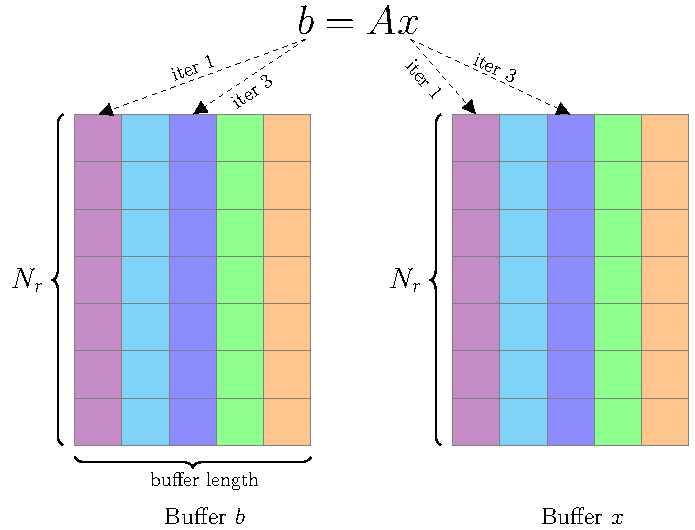
\includegraphics[scale=0.5]{pics/results/symm_spmv_setup/test_setup}
%	\caption{Benchmark \acrshort{SymmSpMV} test setup. \CAcomm{Maybe can ommit this fig.}}
%\end{figure}

{\GW Das passt hier nicht hin und muss uU ausfuehrlicher an anderer Stelle beschrieben werden  Our method has been implemented and consolidated into a library named \acrshort{RACE}. The library provides easy interface for parallelizing kernels having dependencies, user typically just needs to supply a callback function with the serial code (potentially with dependency) and specify the required hardware settings. Library will then parallelize and run the code in parallel. The library is made publicly available through the git repository.}  %TODO
 
%In the following we present the results of two important benchmarks which makes use of the \acrshort{SymmSpMV} and \acrshort{SymmKACZ} kernels. The benchmarks are carefully constructed to mimic the actual settings in real application runs. These benchmarks results are further compared with current state of art alternative methods.
 %Both the benchmarks are run on the full set of test matrices (see \cref{table:bench_matrices}) and the matrices are preprocessed with \acrshort{RCM} bandwidth reduction using the \SPMP library \cite{SpMP}.
%\subsection{Benchmark - \acrshort{SymmSpMV}}
%Sparse matrix vector multiplication is a frequently used operator in plenty of sparse numerical algorithms and is commonly the most time consuming one. This simple benchmark performs multiplication of a symmetric matrix with a vector, and involves a direct use of the \acrshort{SymmSpMV} kernel.  In this benchmark we store only the upper triangular part of the symmetric matrix and perform the full matrix vector multiplication as shown in \cref{sect:SymmSpmv}. 
%The main purpose of this benchmark is to study the performance quality of the \acrshort{RACE} library and make a solid performance-only comparison between different methods, which is made possible due to the exact nature of the \acrshort{SymmSpMV} kernel.
%\subsubsection{Test setup}

\subsection{Results}
Before we evaluate the performance across the full set of matrices presented in \cref{table:bench_matrices} we return to the analysis of \acrshort{SymmSpMV} performance and data traffic for the Spin-26 matrix  which we have presented for the existing coloring approaches in \cref{Sec:motivation}. 
%
\subsubsection{Analysis of \acrshort{SymmSpMV} kernel using RACE with Spin-26 matrix}
%
The shortcomings in terms of performance and excessive data transfer for parallelization of \acrshort{SymmSpMV} using coloring approaches (MC, ABMC) have been demonstrated in \cref{fig:motivation}. We extend this evaluation by comparison with the \acrshort{RACE} results in \cref{fig:motivation_w_RACE}.
 \begin{figure}[thbp]
 	\centering
 	% 	\subfloat[\acrshort{SpMV}]{\label{fig:motivation_spmv}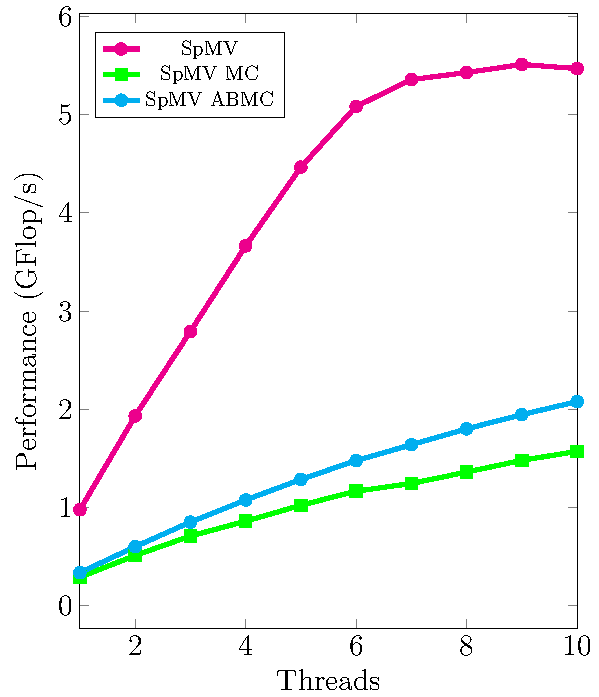
\includegraphics[width=0.26\textwidth, height=0.22\textheight]{pics/motivation/out/motivation_spmv}}
 	%	\hspace{1em}
 	\subfloat[SymmSpMV]{\label{fig:motivation_symm_spmv_w_RACE}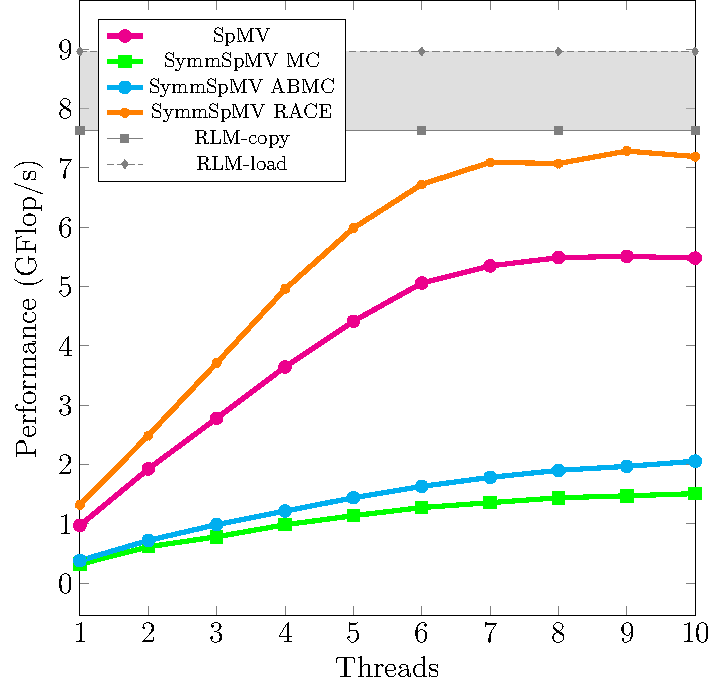
\includegraphics[width=0.38\textwidth, height=0.22\textheight]{pics/motivation/out/motivation_symm_spmv_w_RACE}}
 	\hspace{1em}
 	\subfloat[Data Traffic]{\label{fig:motivation_data_w_RACE}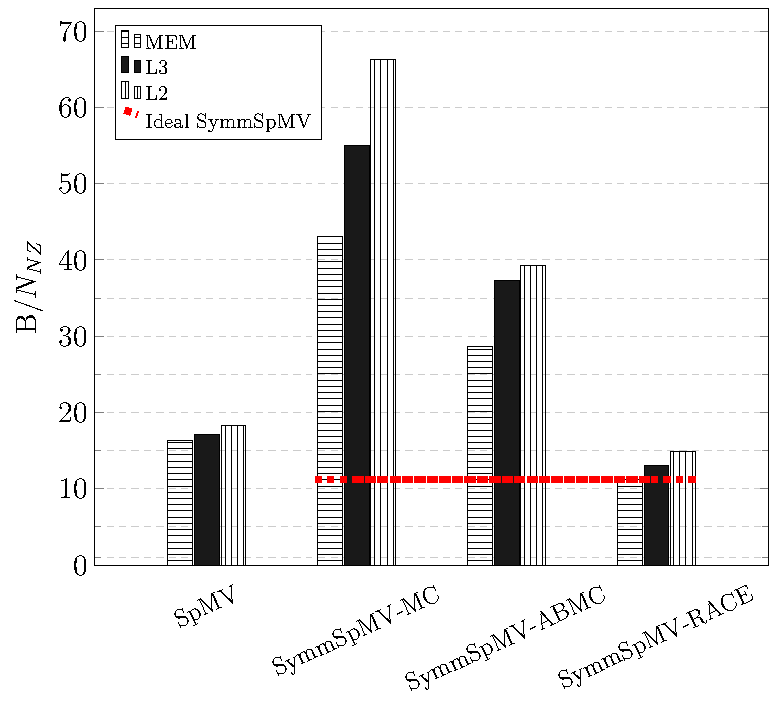
\includegraphics[width=0.4\textwidth, height=0.22\textheight]{pics/motivation/out/motivation_data_w_RACE}}
 	\caption{Performance (left panel) and data traffic analysis (right panel) for \acrshort{SymmSpMV} kernel with Spin-26 matrix using \acrshort{MC}, \acrshort{ABMC} and \acrshort{RACE} on a single socket of \IVB. The roofline performance model (using copy and load-only bandwidth) and the performance of the \acrshort{SpMV} kernel is plotted for reference (left panel). The average data traffic per non-zero entry ($\acrshort{NNZR}$) of the full matrix as measured with \LIKWID for all cache levels and main memory is shown together with the minimal value for main memory access (horizontal dashed line) in the right panel.}
 	\label{fig:motivation_w_RACE}
 \end{figure}
The figures clearly demonstrate the ability of \acrshort{RACE} to ensure high data locality in the parallel \acrshort{SymmSpMV} kernel. The actual main memory traffic achieved is inline with the minimum traffic for that matrix (see discussion in \cref{Sec:motivation}) and a factor of up to 4$\times$ lower than the coloring approaches. Correspondingly \acrshort{RACE} \acrshort{SymmSpMV} performance is 3.5$\times$ higher than its competitors and 40\% better than the \acrshort{SpMV} kernel. It achieves more than 90\% of the roofline performance limit based on the copy main memory performance. Note, that the indirect update of the left hand side vector will generate a store instruction for every inner loop iteration (see \cref{alg:SymmSpMV}), while the \acrshort{SpMV} kernel only does a final store at the end of the inner loop iteration. In combination with the low number of non-zeros of the Spin-26 matrix, the "copy" induced limit poses a realistic upper performance bound.  
%
\subsubsection{Analyzing absolute performance of RACE}
%
We now extend our \acrshort{RACE}  performance investigation to the full set of test matrices presented in~\cref{table:bench_matrices}. In \cref{fig:spmv_vs_symm_spmv_ivy,fig:spmv_vs_symm_spmv_skx} the performance results for the full \IVB processor chip (10 cores) and the full \SKX processor chip (20 cores) are presented along with the upper roofline limits and the performance of the baseline \acrshort{SpMV} kernel using \acrshort{MKL}.  
 \begin{figure}[thbp]
	\centering
	\subfloat[\IVB]{\label{fig:spmv_vs_symm_spmv_ivy}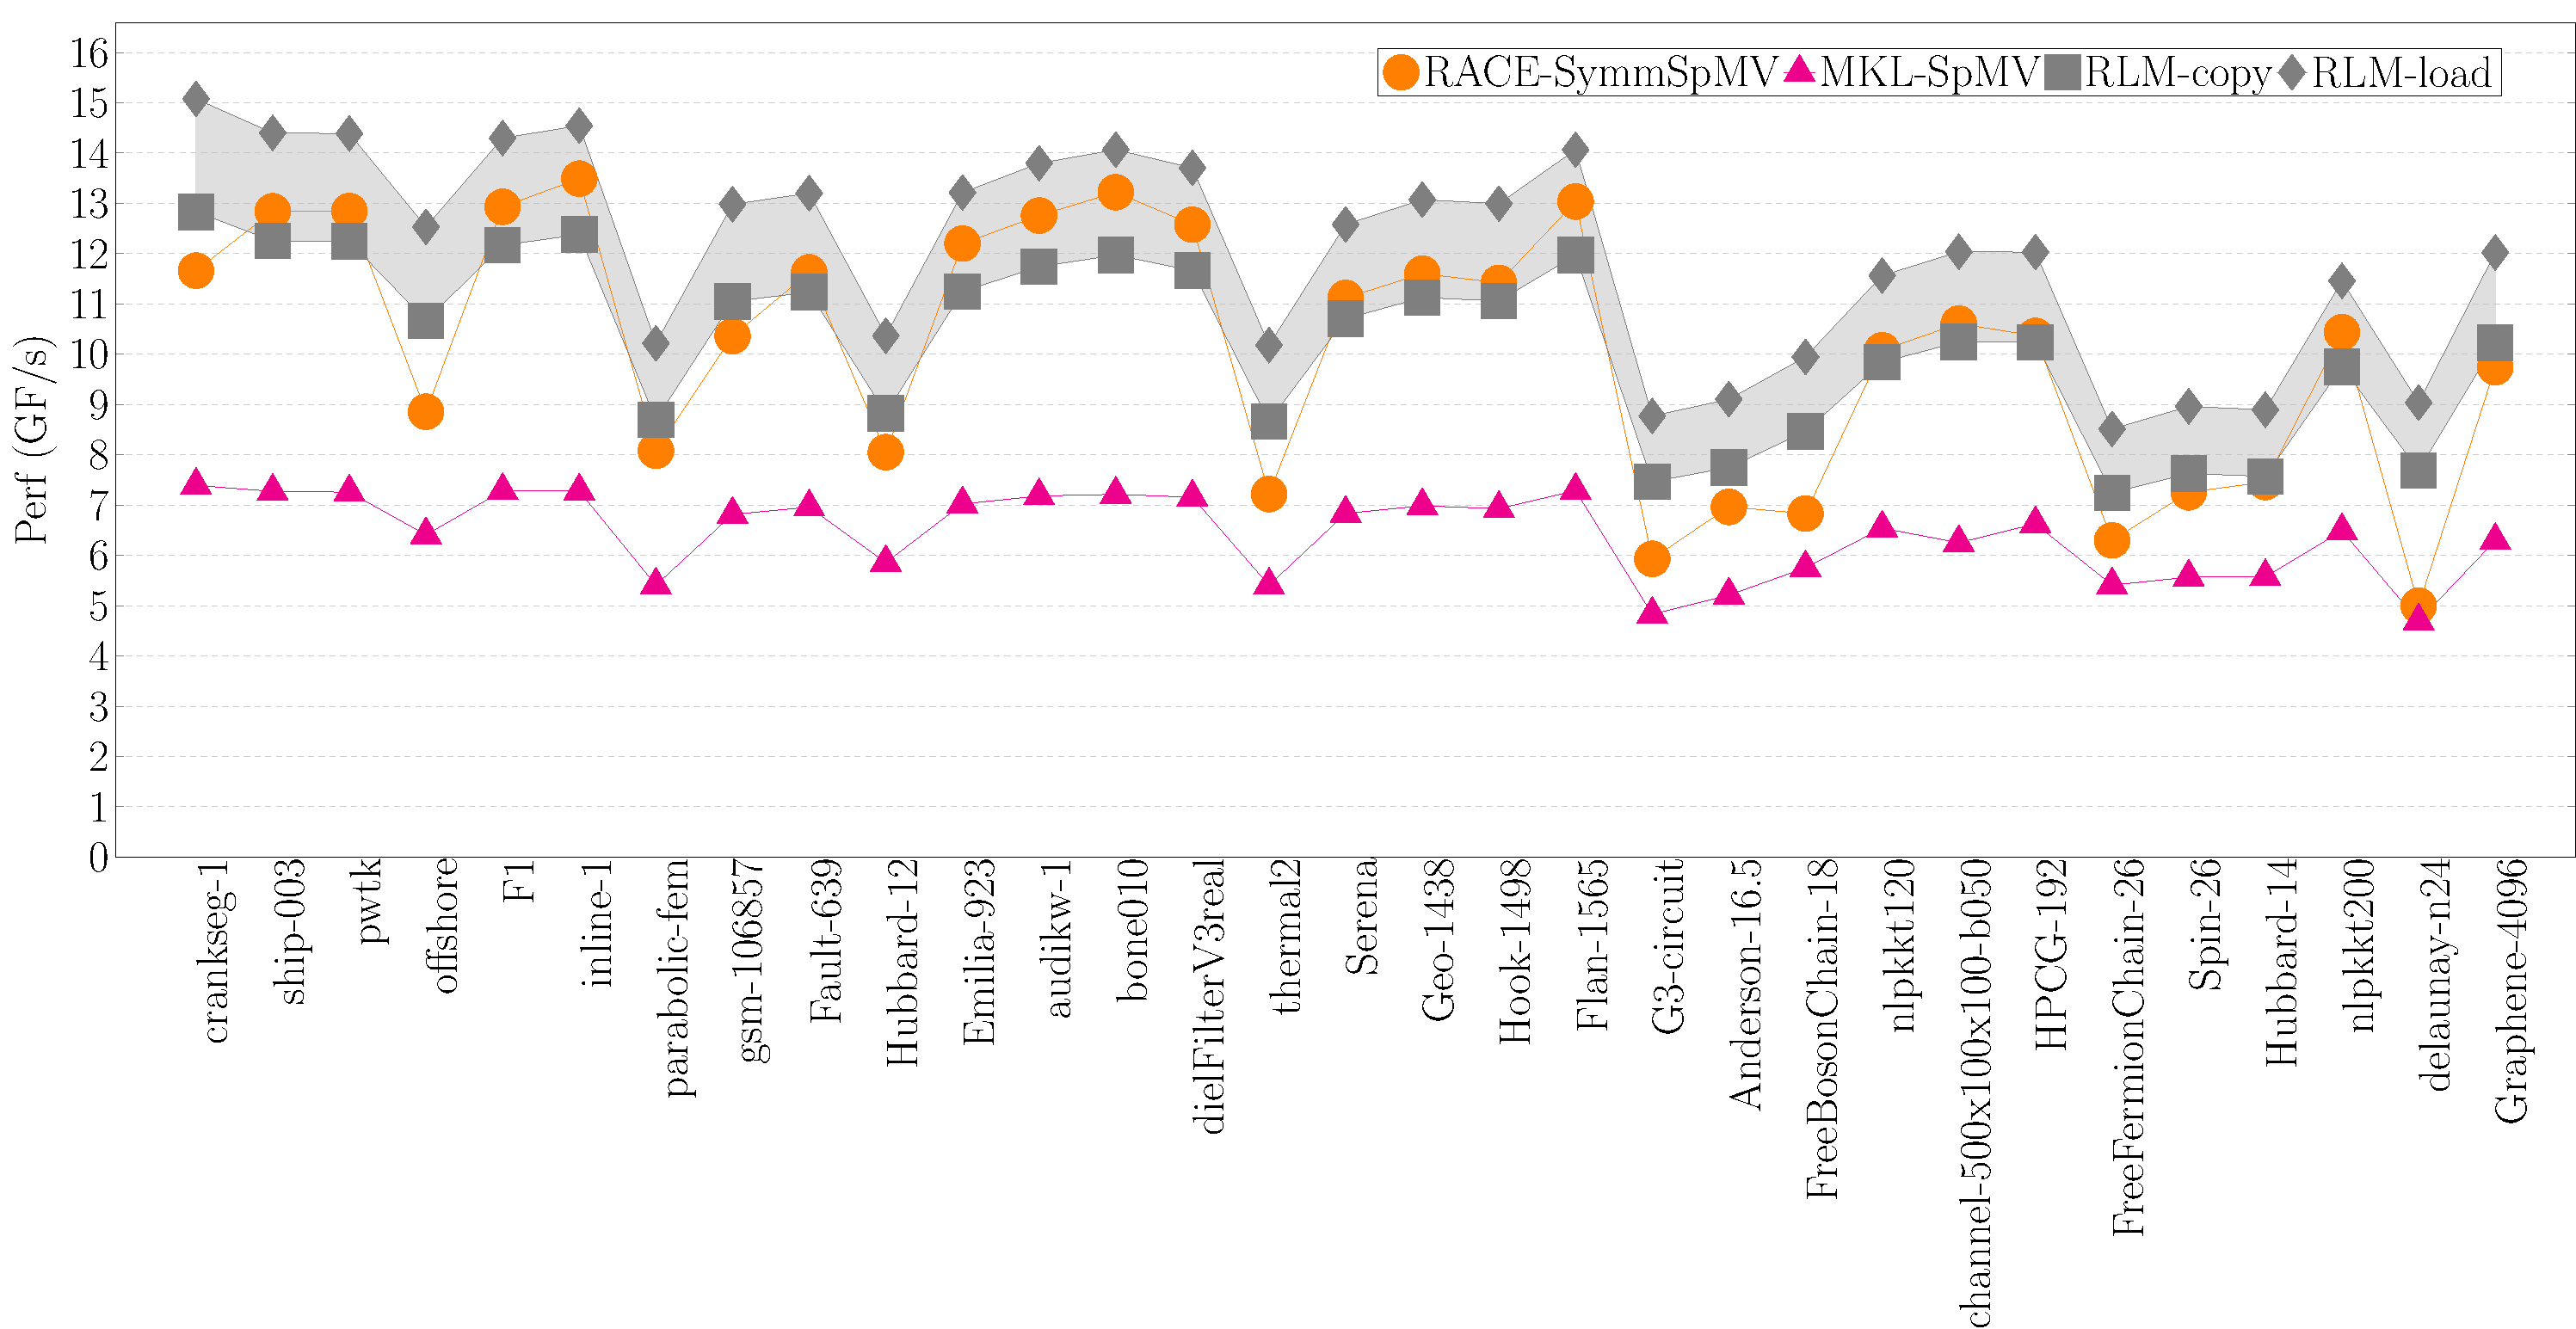
\includegraphics[width=0.85\textwidth, height=0.27\textheight]{pics/results/ivy/data_symm_spmv/plot_generator/perf_vs_mtx_RACE_w_SpMV/perf}}
	\hspace{1em}
	\subfloat[\SKX]{\label{fig:spmv_vs_symm_spmv_skx}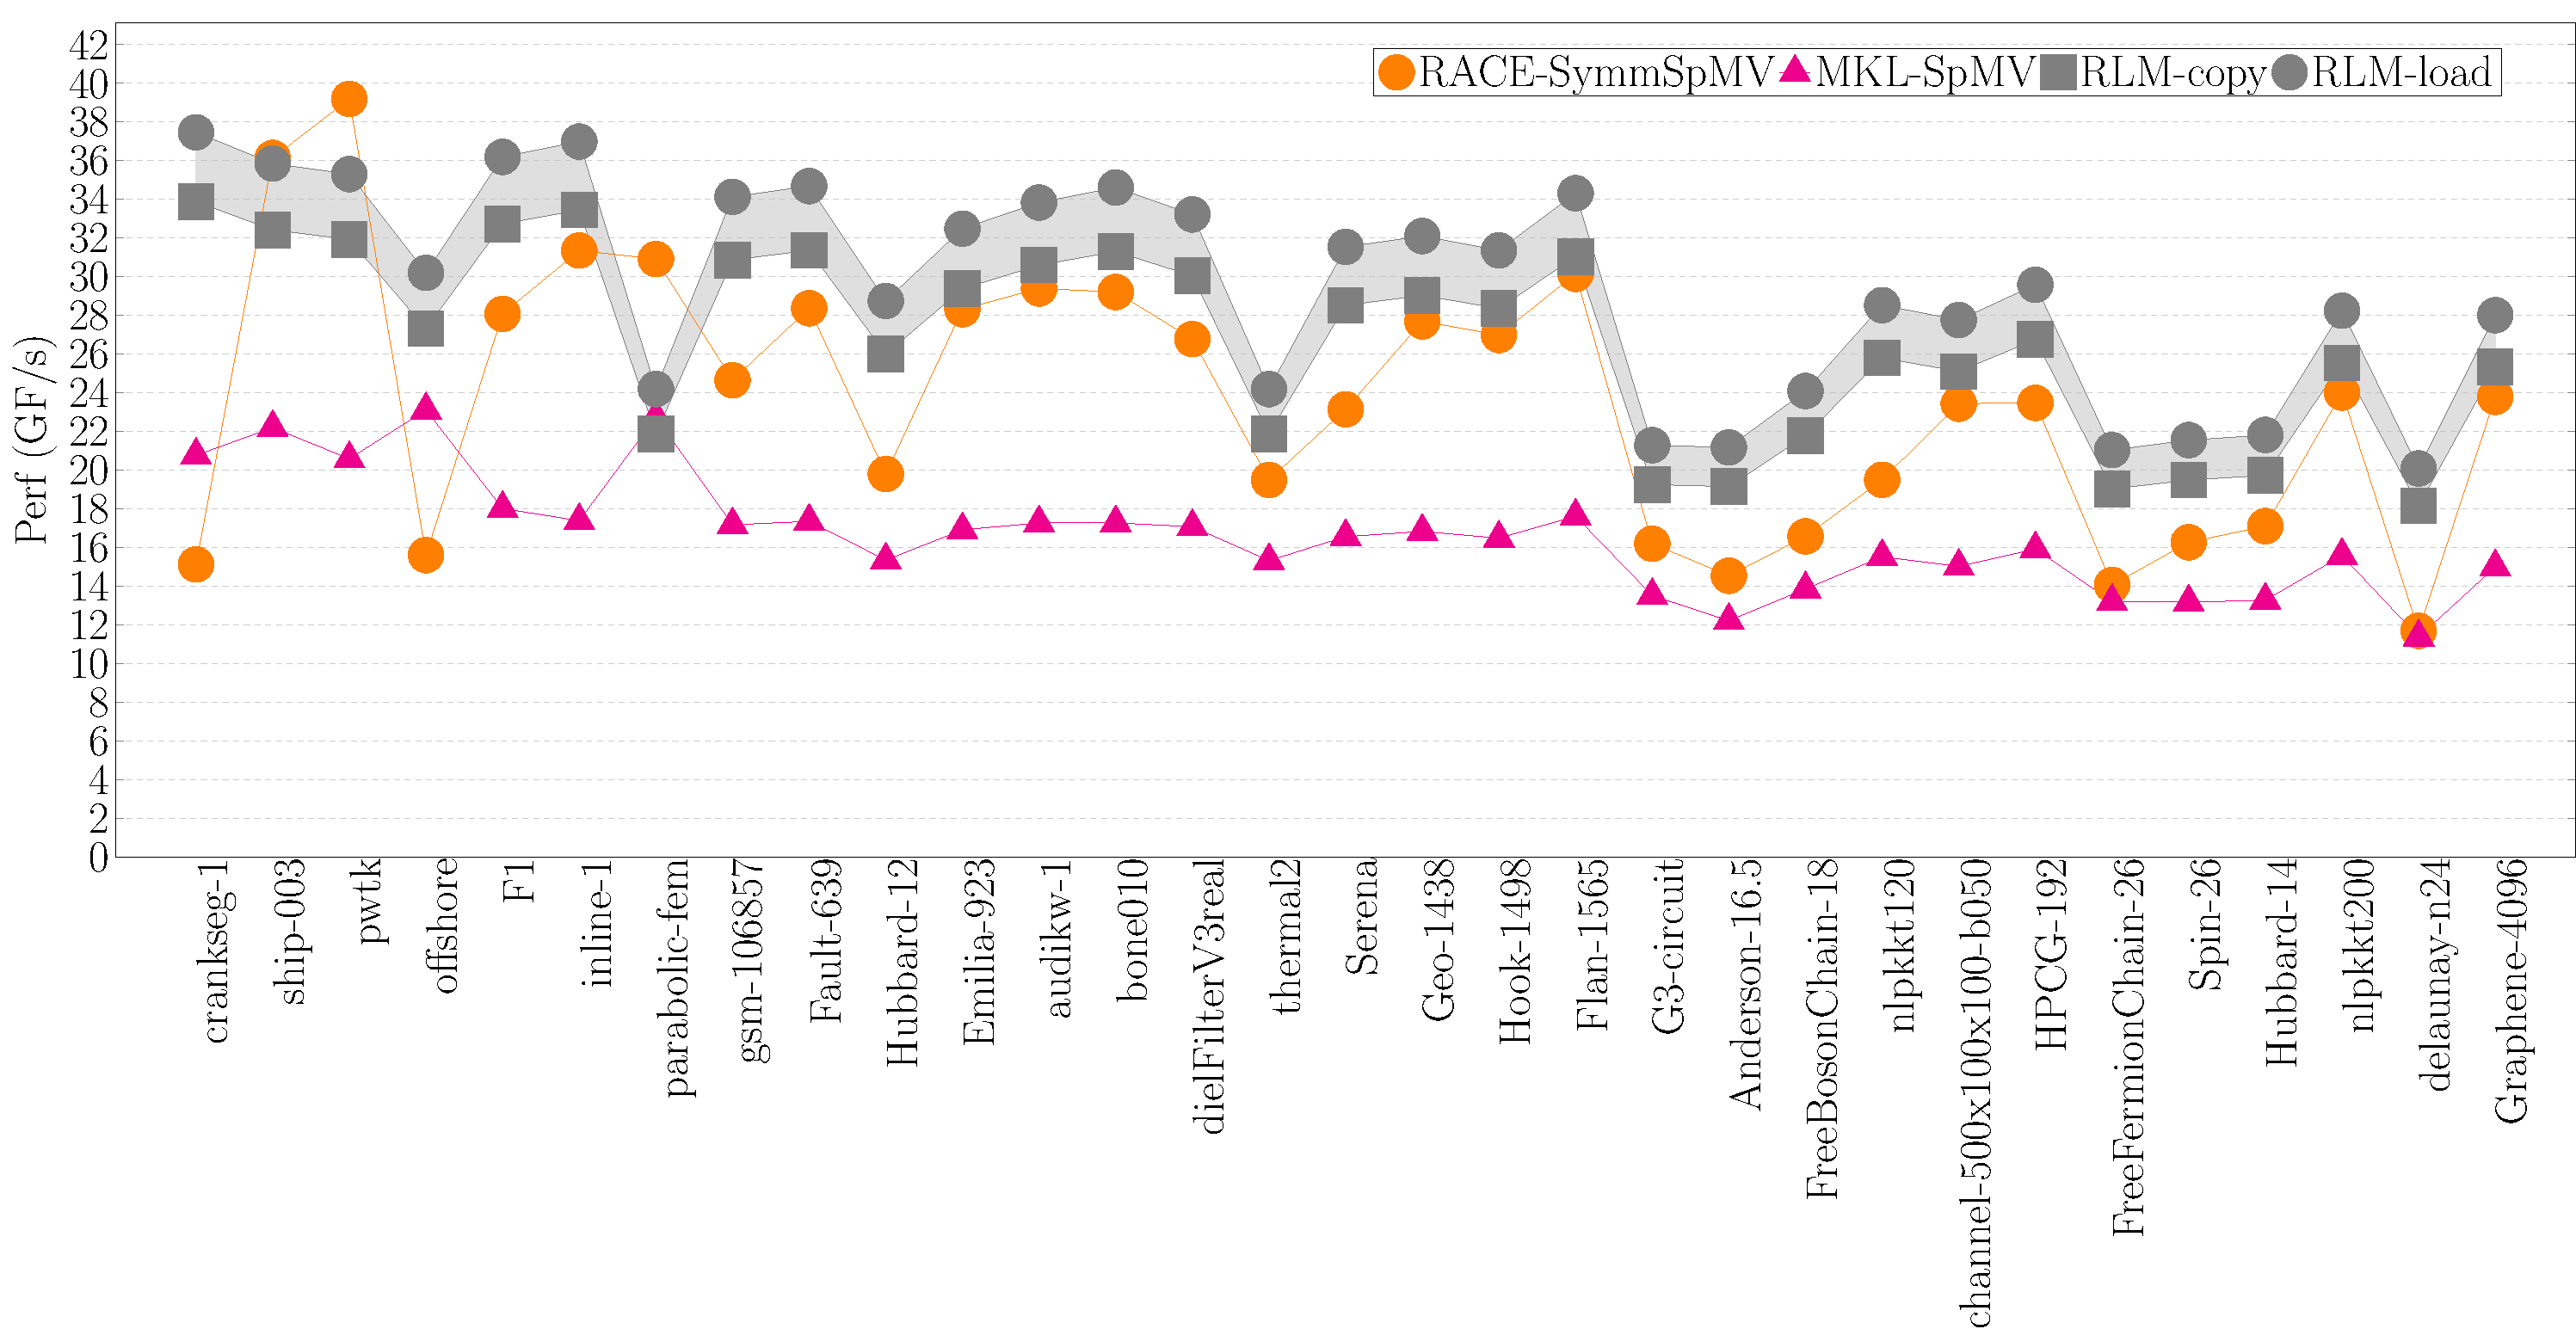
\includegraphics[width=0.85\textwidth, height=0.27\textheight]{pics/results/skx/data_symm_spmv/plot_generator/perf_vs_mtx_RACE_w_SpMV/perf}}
	\caption{Performance of \acrshort{SymmSpMV} executed with \acrshort{RACE} compared to performance model. \acrshort{SpMV} performance obtained using \acrshort{MKL} library is also shown for reference.}
	\label{fig:SpMV_vs_SymmSpMV}
\end{figure}
The matrices are arranged along the abscissa according to the ascending number of rows (\acrshort{nrows}), i.e. increasing size of the two vectors involved in \acrshort{SymmSpMV}. Overall \acrshort{RACE}  performance comes close or matches our performance model for many test cases on both architectures. 
A characteristic drop in performance levels is encountered around the \texttt{Flan\_1565} and \texttt{G3\_circuit} matrices, where the aggregate size of the two vectors (25 MB) approaches the available cache size on both architectures. For smaller matrices we have a higher chance that the vectors stay in the cache during the \acrshort{SymmSpMV}, while for larger matrices the vectors may be loaded several times. This is qualitatively reflected by the measured $\alpha_{\acrshort{SpMV}}$ values presented in \cref{table:alpha_values}. 

We further find performance drops both for measurements and model prediction which have a strong correlation with lower \acrshort{SpMV} performance, e.g. \texttt{Hubbard-12}, \texttt{thermal2} or \texttt{delauny\_n24}. These matrices are characterized by a rather low $\acrshort{NNZR}$ and extremely high bandwidth indicating strongly irregular access to the two vectors. This is reflected in the increased $\alpha_{\acrshort{SpMV}}$ value and the corresponding low roofline performance limits. Note, that  $\alpha_{\acrshort{SpMV}}$ is measured for \acrshort{SpMV}  kernel mainly accounts for the RHS vector traffic. Thus it is an optimistic upper bound for the actual data traffic in the \acrshort{SymmSpMV} kernel, which requires two vectors to stay in cache concurrently.  

The \texttt{crankseg\_1} and \texttt{offshore} matrices have a qualitatively different behavior on both architectures, which is caused by the limited amount parallelism in these structures. Here we refer to the discussion of \cref{fig:crankseg_param} where best performance and highest parallelism (\acrshort{threadEff}) was achieved at approximately 10 cores. 

{\GW Stopped HERE} 


\Inorder to further verify the quality of our method we compare the results of this benchmark against the performance predictions for all the test matrices (see \cref{table:bench_matrices}). \Cref{fig:spmv_vs_symm_spmv_ivy,fig:spmv_vs_symm_spmv_skx} show this results for \IVB and \SKX architecture respectively. 

The performance model is constructed using \cref{eq:upper_performance} and the intensity equation seen in \cref{eq:SymmSpMV_intensity}, the $\alpha$ value of the reference \acrshort{SpMV} kernel is taken into account. The measured $\alpha$ values for the matrices and the two architectures are shown in \cref{table:alpha_values}. The plots show close agreement of the \acrshort{RACE} performance and the predictions. Even though the performance model should give upper limit for performance there are two outliers on \SKX architectures namely \emph{pwtk} and \emph{parabolic\_fem}, which as discussed previously in \cref{subsec:param_analysis} is due to the fact that these matrices are small enough to fit in the cache of this architecture. The performance of \emph{offshore} matrix reflects same behavior as \emph{crankseg-1} due to the load imbalance problem as discussed earlier.


From the model and measurements it is well clear that even though \acrshort{SymmSpMV} requires theoretically only half the memory data volume it is not always the case we achieve two times the performance even for well memory-bound cases. This is due to the bigger pre-factor of the $\alpha$ term for \acrshort{SymmSpMV} compared to \acrshort{SpMV} ($24$ vs $8$ respectively).

%
\subsubsection{Comparing RACE with other methods}
%

Having well understood the performance of \acrshort{RACE} we now compare \acrshort{SymmSpMV} benchmark with the other methods. Here we will compare the performance with coloring methods \acrshort{MC} and \acrshort{ABMC} that were previously discussed and also with the widely used math numerical library \acrshort{MKL}.  We use the same libraries and setup as mentioned in  \cref{Sec:motivation} for pre-processing the matrix with \acrshort{MC} and \acrshort{ABMC} methods. The methods are then executed with the same inner kernel \acrshort{SymmSpMV} as used for \acrshort{RACE}.  

\begin{figure}[thbp]
	\centering
	\subfloat[\IVB]{\label{fig:symm_spmv_ivy}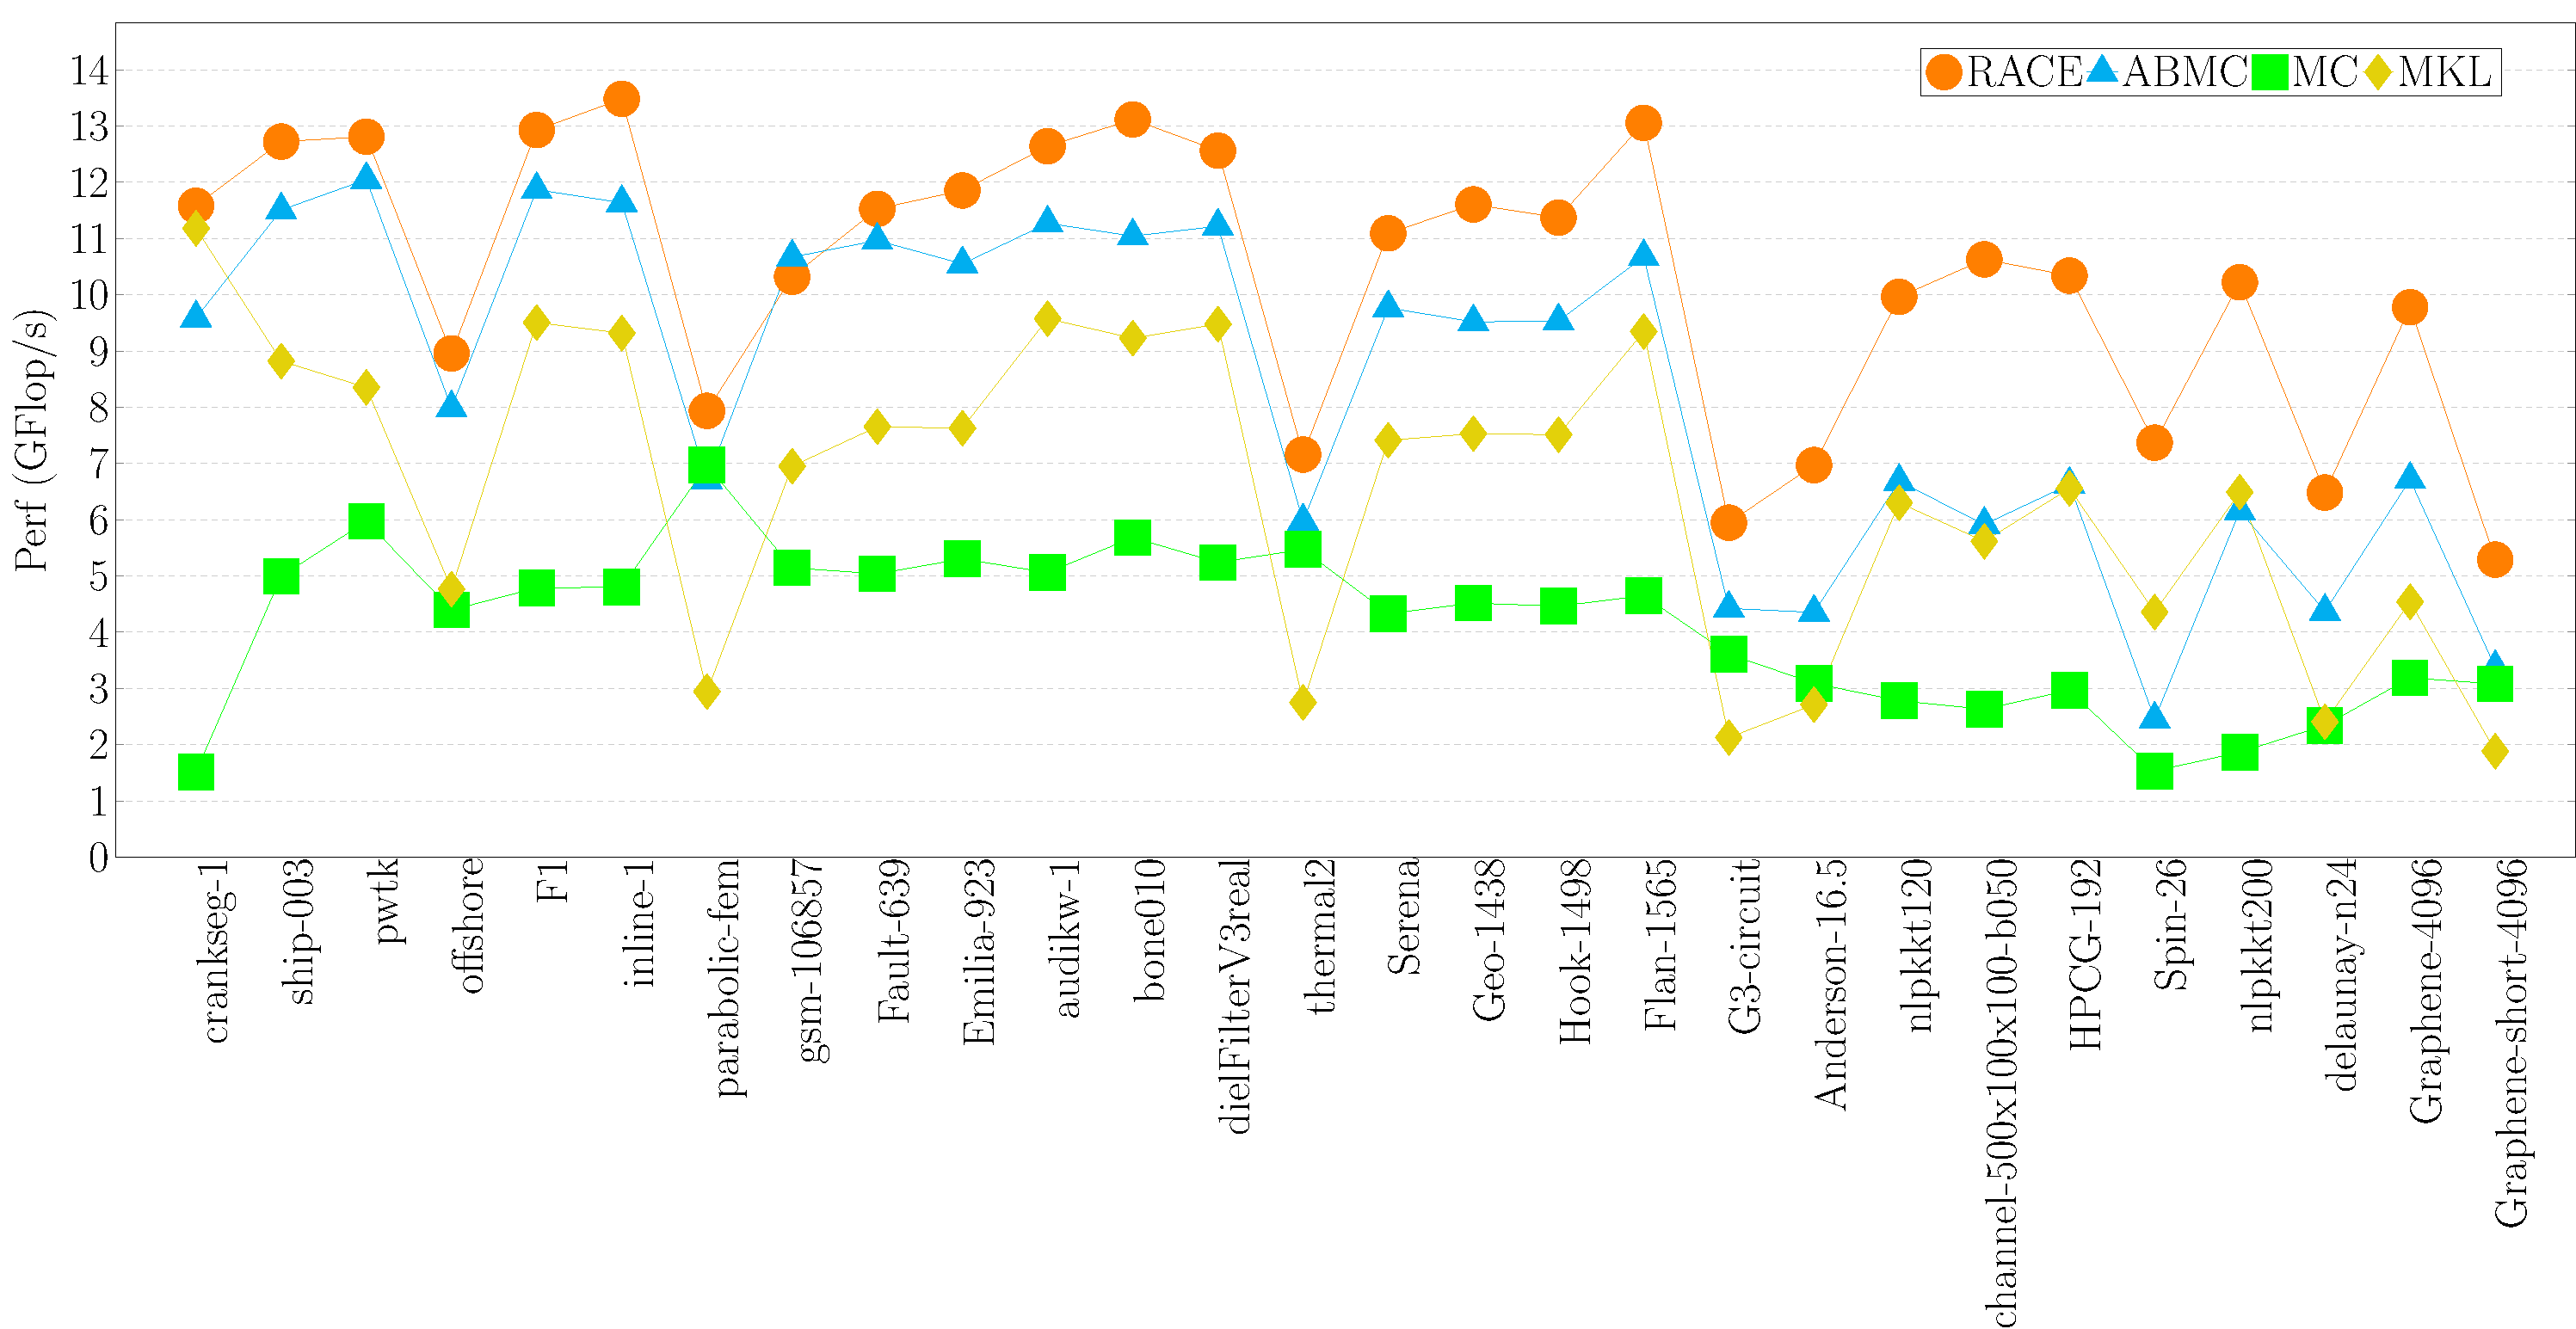
\includegraphics[width=0.85\textwidth, height=0.27\textheight]{pics/results/ivy/data_symm_spmv/plot_generator/perf_vs_mtx/perf}}
	\hspace{1em}
	\subfloat[\SKX]{\label{fig:symm_spmv_skx}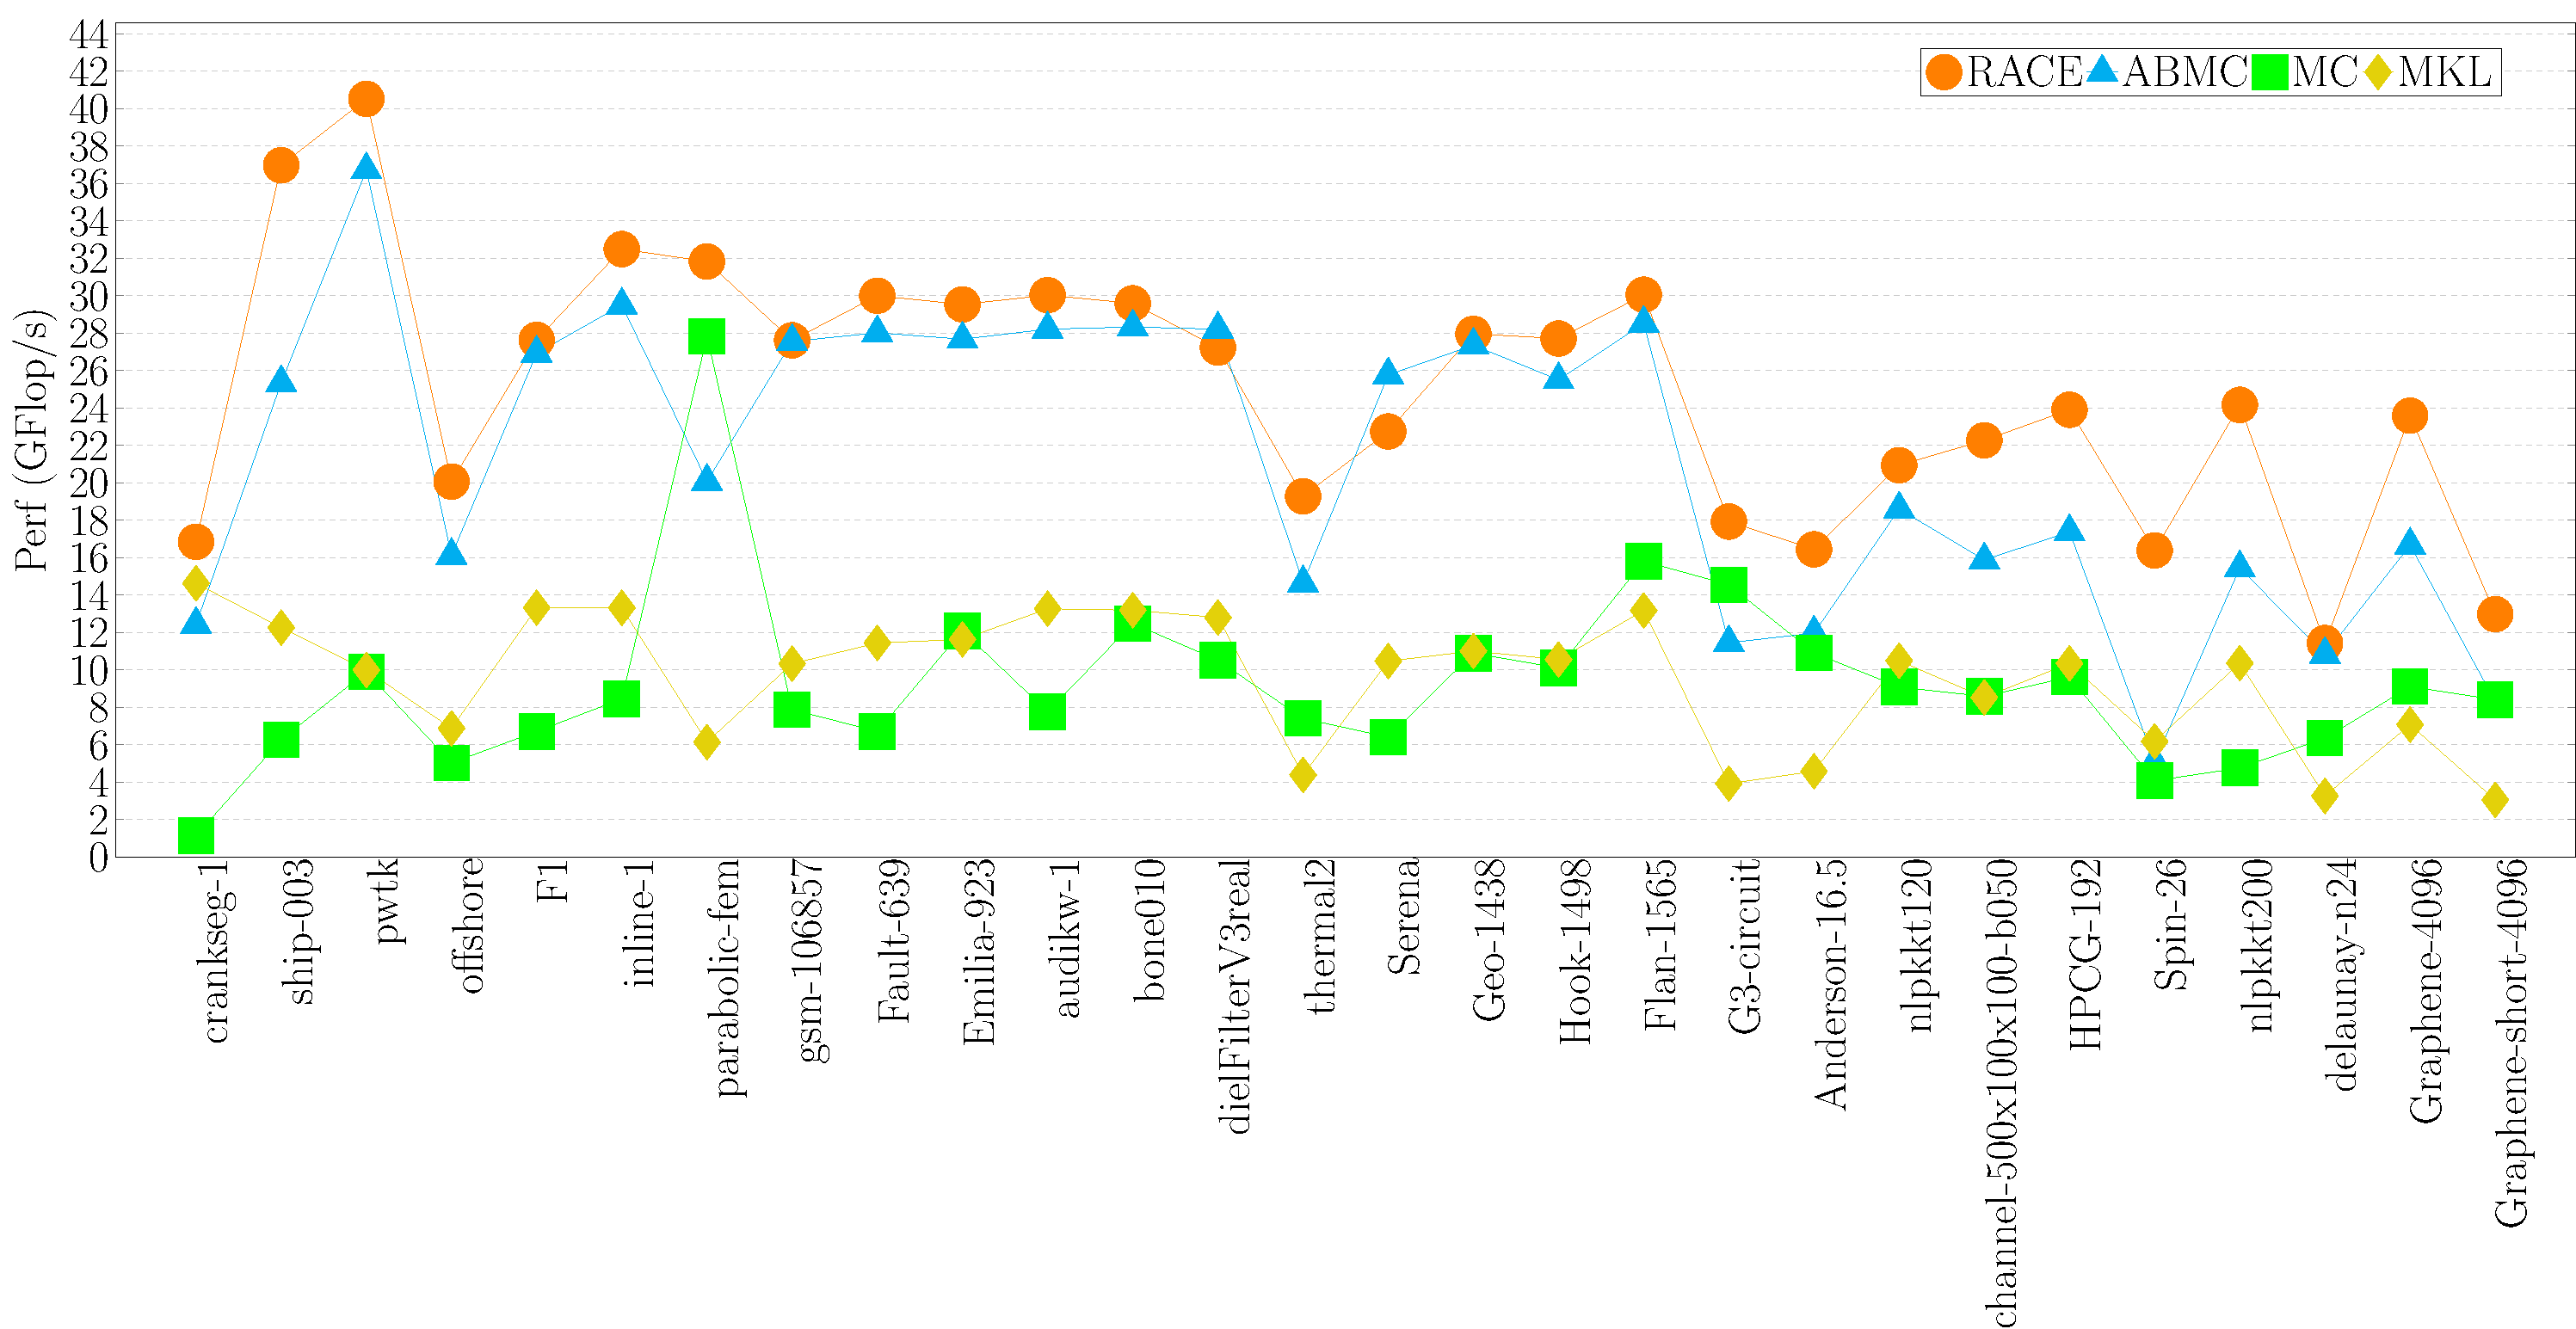
\includegraphics[width=0.85\textwidth, height=0.27\textheight]{pics/results/skx/data_symm_spmv/plot_generator/perf_vs_mtx/perf}}
	\caption{Comparison of \acrshort{SymmSpMV} performance obtained using various implementations. Matrices arranged in increasing number of rows (\acrshort{nrows}).}
	\label{fig:symm_spmv}
\end{figure}

For \acrshort{MKL} we use two available implementations that does \acrshort{SymmSpMV} operation. The first one is the \texttt{mkl\_cspblas\_dcsrsymv} kernel where it directly computes the product of the given sparse triangular matrix and a vector. However this kernel has been deprecated from \acrshort{MKL}.v.18 and a newer routine under Inspector-executor Sparse BLAS is to be used. In the newer method user initially provide the matrix along with hints (symmetry) and operations to be carried out. Then the optimize routine is called where the matrix could be pre-processed based on the hint and the required operation. Finally the kernel \texttt{mkl\_sparse\_d\_mv} is executed on this optimized matrix to perform the matrix vector multiplication. By this method one has no guarantee what kernel the library uses under the hood, for example the library can even change the data storage format internally and use respective kernel.

Results of these comparisons are shown in \cref{fig:symm_spmv}. The matrices are arranged according to ascending number of rows (\acrshort{nrows}). Clearly in all the cases \acrshort{RACE} has an upper hand compared to other methods. \acrshort{ABMC} method comes next followed by \acrshort{MKL} and \acrshort{MC} methods. Speedup gained by the \acrshort{RACE} method is higher for matrices towards right since the dimension \acrshort{nrows} is large such that the whole right hand side vector $x$ do not fit into cache anymore, as a result of this the data locality of the method plays a more important role for these matrices towards right as it directly impacts memory traffic. Even though both \acrshort{MKL} versions do not have an on par performance compared to \acrshort{RACE} it is interesting to note that the Inspector-Executor version of \acrshort{MKL} (MKL-IE) has exactly the same performance of a general MKL-\acrshort{SpMV} as seen previously in \cref{fig:SpMV_vs_SymmSpMV}. This we believe is due to the fact that internally the library decides the implementation of \acrshort{SymmSpMV}  is not beneficial and switches to \acrshort{SpMV} kernel. We further validated this by measuring the memory data volume using \LIKWID, which shows almost twice the data volume compared to \acrshort{SymmSpMV}.

The overall speedup of \acrshort{RACE} over the next best performing variant \acrshort{ABMC} is $1.5\times$ and $1.65 \times$ for \IVB and \SKX respectively, whereas for some matrices the speed-up is higher than $3 \times$. Compared to other methods we constantly have a speedup of more than $2.5 - 3 \times$ in most of the cases. 

\subsection{Benchmark - \acrshort{SymmKACZ}}
Kaczmarz solver is a stable and very robust iterative solver, but the convergence of the solver for many cases are very slow. Therefore in most of the scientific simulations a conjugate gradient (CG) accelerated variant of the Kaczmarz solver known as CGMN \cite{CGMN} is used. The CGMN solver has been found to be very efficient and robust solver for a wide range of linear systems \cite{CGMN_gordon}. In this benchmark we test the CGMN solver with different parallel implementations of \acrshort{SymmKACZ} kernel. 

The main purpose of this benchmark is to study an inexact iterative kernel where the convergence depends on the parallelization scheme used. The benchmark compares performance, convergence and time to solution of different coloring methods.

\subsubsection{Test setup}
The CGMN algorithm is implemented as shown in \cite{CGMN_gordon}. The algorithm involves couple of BLAS-1 calls that constitute less than 10\% of total runtime and the time intensive \acrshort{SymmKACZ} kernel. The linear system of equation to be solved is setup such that the exact solution ($x$) is a pure diagonal vector with all elements set to 10 (\ie [10,10,10,...]).

With the change in order of rows to be calculated (for \eg by permutation) the convergence rate of \acrshort{SymmKACZ} is changed, thereby that of CGMN. \Inorder to fix the baseline convergence we first run a serial version of CGMN algorithm for 100 iterations without using any coloring schemes. The $\ell_2$ norm of the error vector is then computed and fixed as the target error  norm. The parallel versions of the algorithm are then run on the same linear system until it reaches the target error norm. The runtime, mean performance and number of iterations to achieve the target are noted for comparisons.


\subsubsection{Results}

{\GW Will continue here...}


\begin{comment}
\subsection{\acrshort{RACE} performance in comparison to SpMV}



\subsection{Test setup}
In the following we present the performance and convergence results obtained using the library, and compare it against state of art methods. \acrshort{SymmSpMV} and \acrshort{SymmKACZ} are chosen as representative benchmark kernels. Hardware and matrices as described in \cref{Sec:test_bed} is used for the following benchmarks. As mentioned in \cref{Sec:param_study} parameter $\epsilon_s$ is set to 0.8 and \acrshort{RCM} is used in level construction stage. The matrix is pre-processed with \acrshort{RCM} for all the cases (even for \acrshort{SpMV}). \SPMP \cite{SpMP} library was used to do this \acrshort{RCM} pre-processing.

The test setup is so constructed that it replicates the behavior of these kernels in actual practical scenarios. Normally matrix vector multiplication is followed by different calls to other kernels that use other helper data. This may lead to eviction of residual data from matrix vector multiplication. In order to replicate this behavior for \acrshort{SymmSpMV} and \acrshort{SpMV} (used as reference) we use  two ring buffers holding vectors of size \acrshort{nrows}. Number of vectors in this ring buffer is chosen such that these two ring buffer occupy a size of 100 \MB, which is at least two times bigger that the combined cache size of the two architectures considered. The kernels are then run two times over these ring buffer, and mean performance of the runs is taken into account.

For \acrshort{SymmKACZ} there are two use cases. In one it is used as a plain iterative solver where the kernel is called successively. The other use case of this iterative solver is in algorithms like CGMN~\cite{CGMN, CGMN_gordon} or CARP-CG~\cite{CARP-CG} where \acrshort{SymmKACZ} is used like a preconditioner, where an approach similar to \acrshort{SymmSpMV} have to be used for benchmarking. In this paper the benchmark is constructed to replicate the behavior of the former case, \ie we call the \acrshort{SymmKACZ} kernel 500 times in succession and report the mean performance. It has to be noted that the difference in performance measurements between these two benchmarks is very small and only affects small matrices.


\subsection{Performance and comparisons}



\Cref{fig:SpMV_vs_SymmSpMV} provides performance of SymmSpMV compared to SpMV. Roofline \cite{Williams_roofline} model for each of the matrices is also shown in the figure. The model takes into account the alpha factor, which is derived based on SpMV performance.

 From the figure one can observe that in some cases roofline performance is lower than that of actual measured performance. This is due to the fact that these are small matrices and some of the data can fit in the cache, since \SKX has cumulatively larger cache compared to \IVB we observe more matrices showing this kind of behavior.
 
 The figure also makes it clear that eventhough we only operate with upper triangle part of the matrix, it is not always the case we get a factor of two in performance. There are basically two reasons for it as suggested by roofline model:
 \begin{enumerate}
 	\item Small non-zeros per row \acrshort{NNZR}: If \acrshort{NNZR} its symmetric variant \acrshort{SymmNNZR} will be even smaller, since this term enters into denominator of $I_{\acrshort{SymmSpMV}}$ as shown in \cref{eq:SymmSpMV_intensity} it decreases the performance even more.
 	\item $\alpha$ factor: The effect of $\alpha$ on \acrshort{SymmSpMV} kernel is more than that of \acrshort{SpMV}. One can observe this by comparing \cref{eq:SpMV_intensity,eq:SymmSpMV_intensity}, where the  pre-factor of $\alpha$ is three times bigger for \acrshort{SymmSpMV}.
 \end{enumerate}



%\begin{comment}

\begin{figure}[thbp]
	\centering
	\subfloat[\acrshort{SymmSpMV} on 1 socket of \IVB]{\label{fig:symm_spmv_ivy_nlpkkt}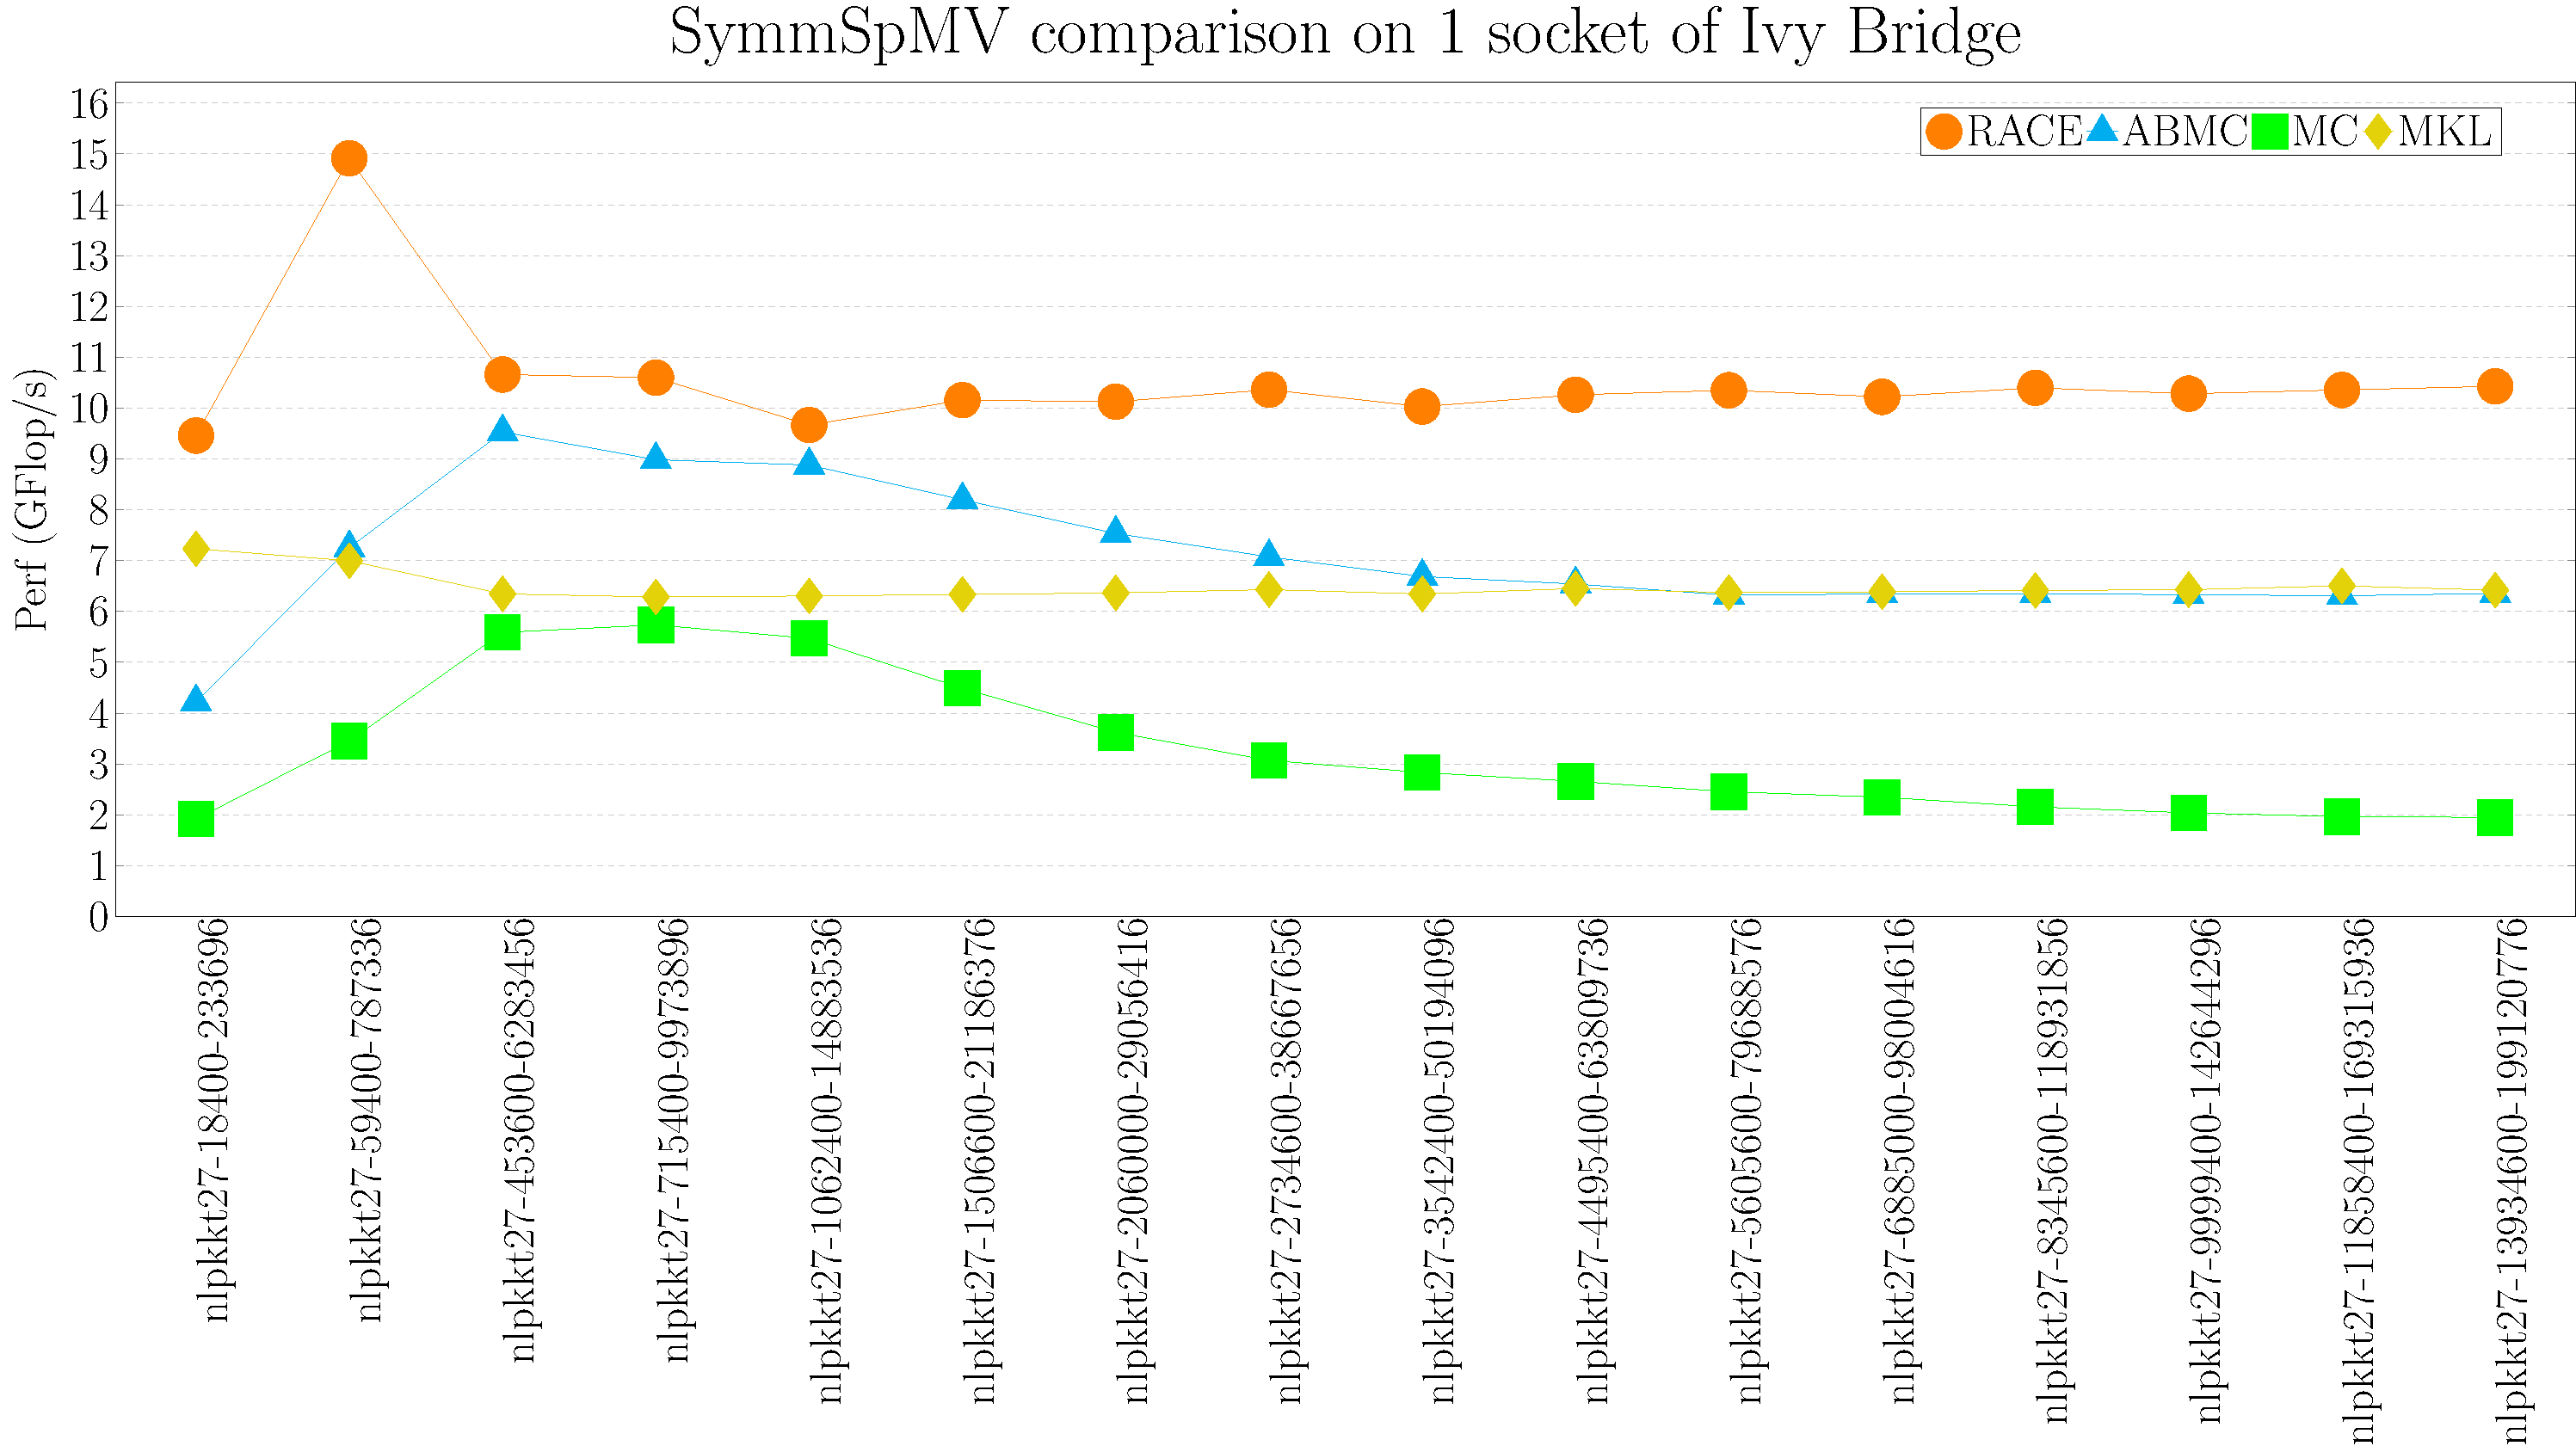
\includegraphics[width=0.48\textwidth, height=0.15\textheight]{pics/results/ivy/data_symm_spmv/plot_generator/perf_vs_mtx/ivy_nlpkkt}}
	\hspace{1em}
	\subfloat[\acrshort{SymmSpMV} on 1 socket of \SKX]{\label{fig:symm_spmv_skx_nlpkkt}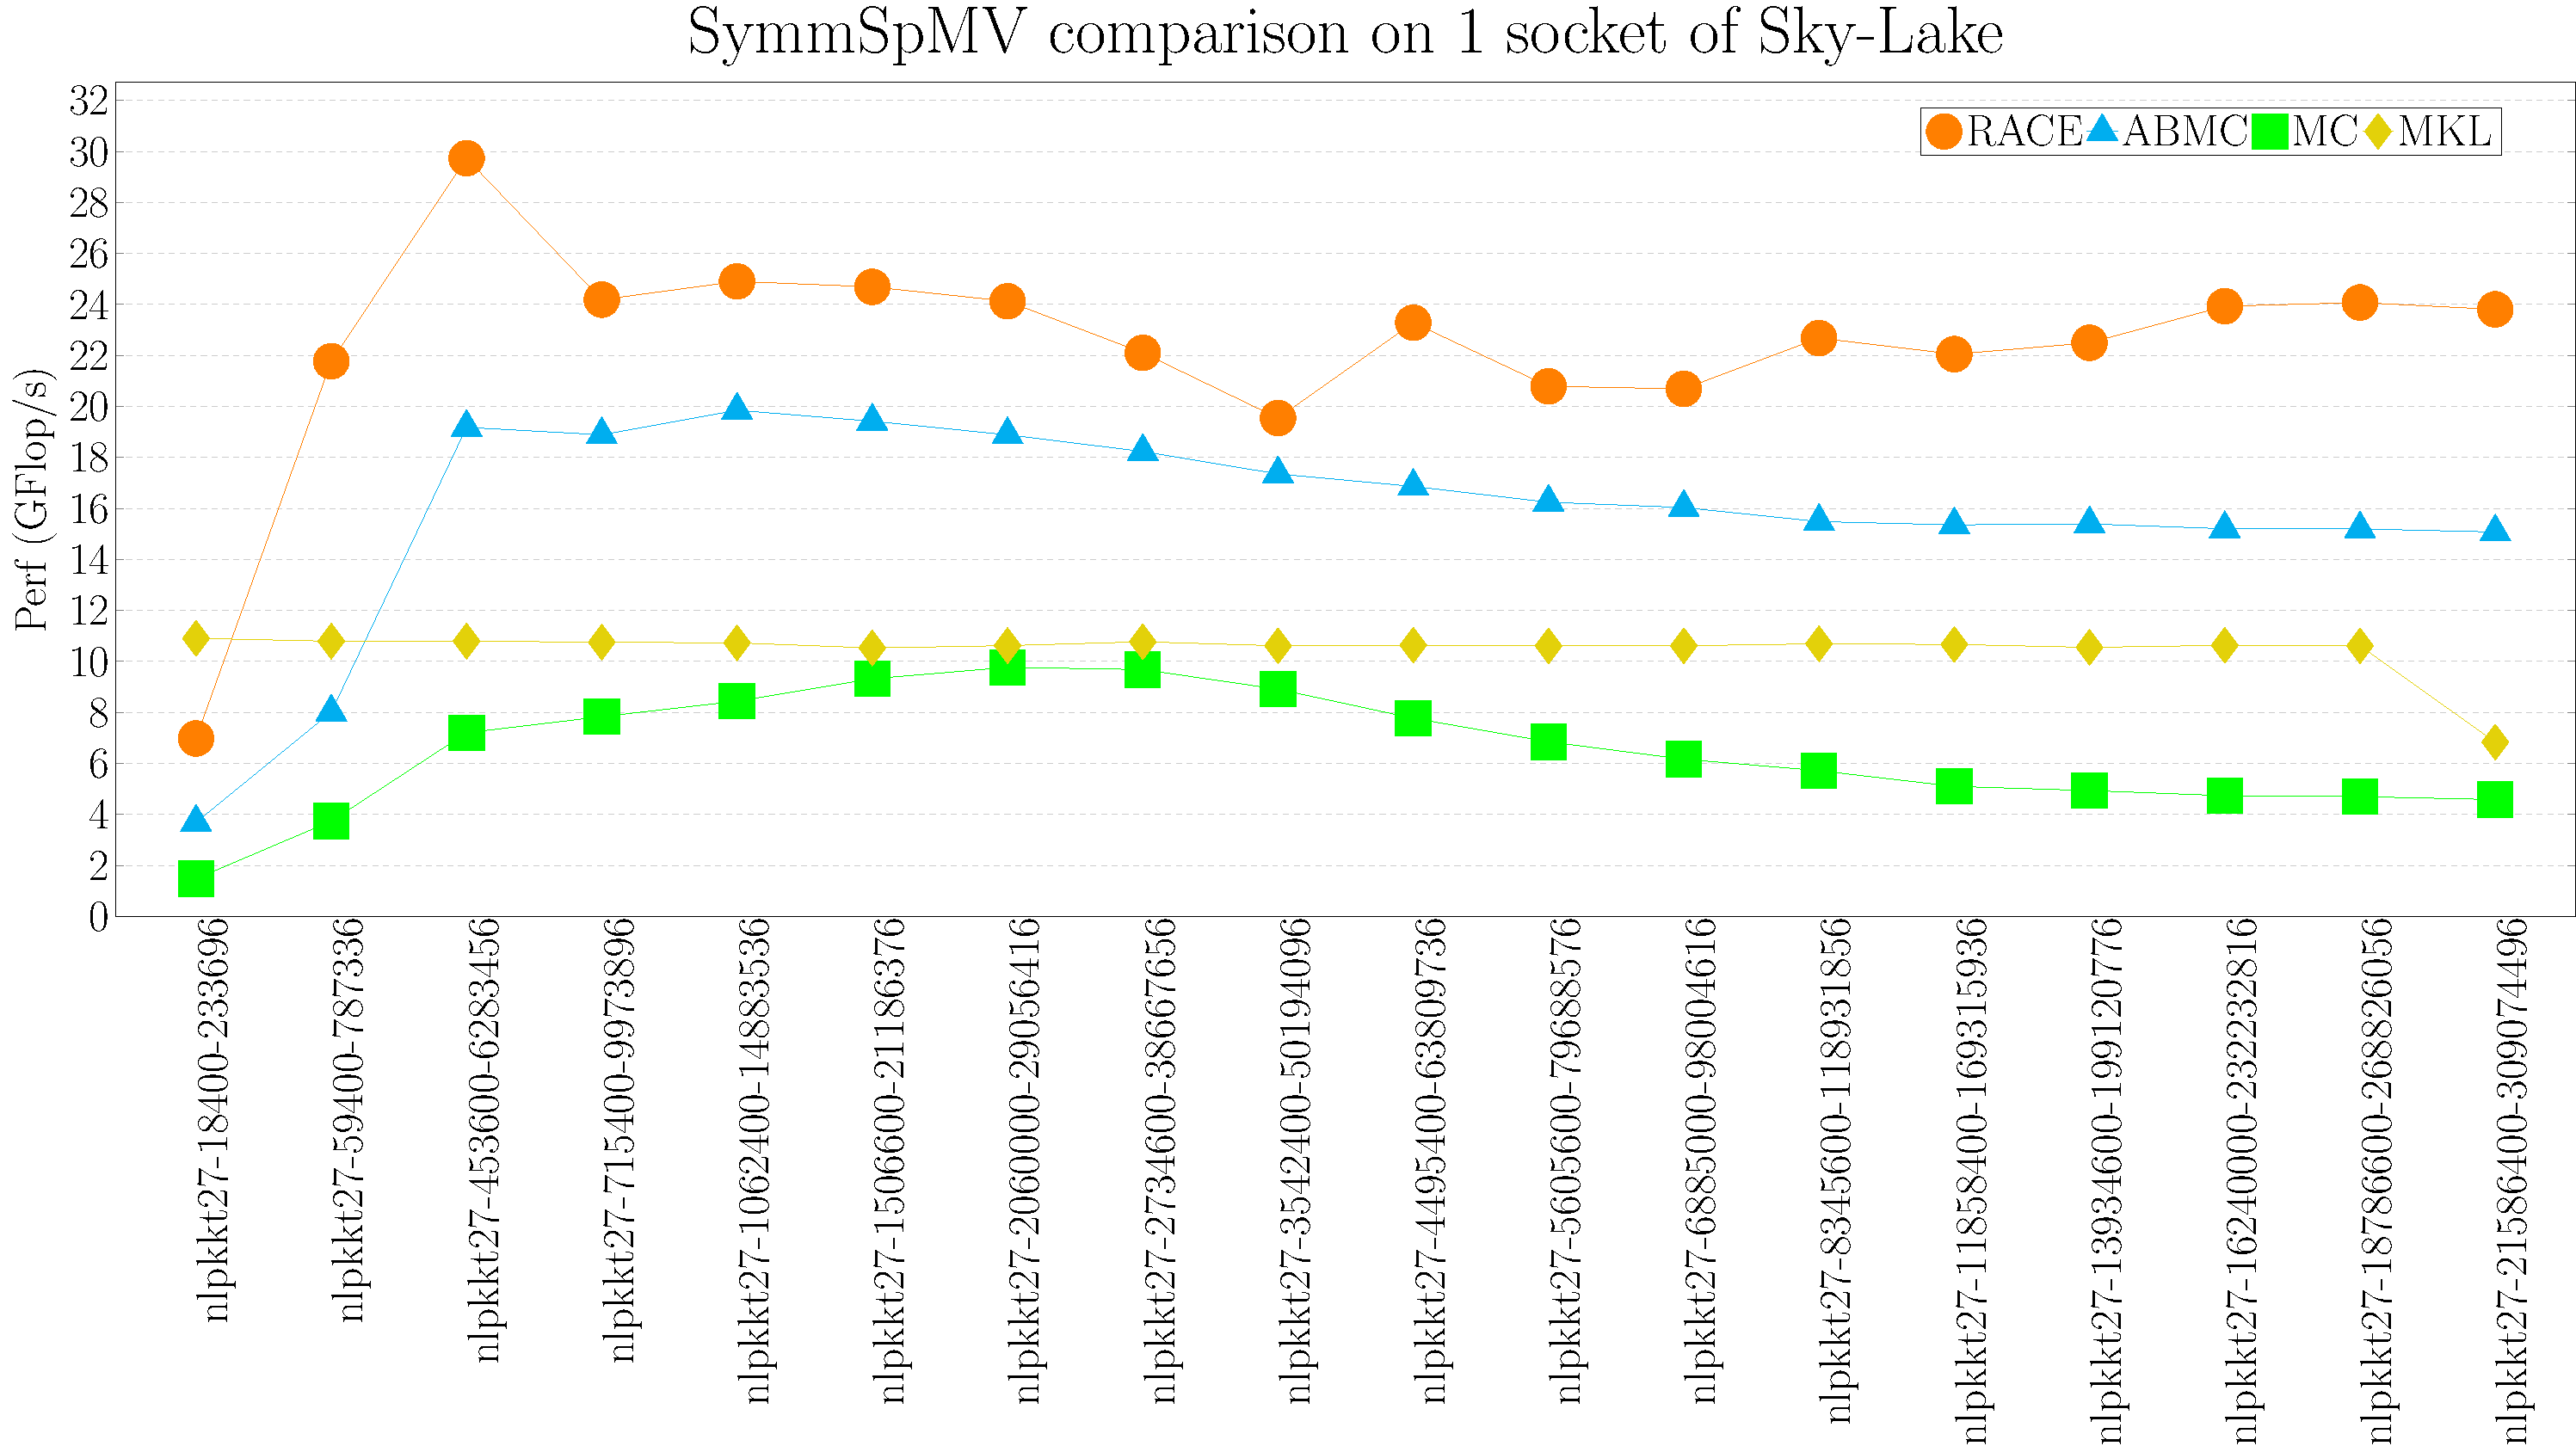
\includegraphics[width=0.48\textwidth, height=0.15\textheight]{pics/results/skx/data_symm_spmv/plot_generator/perf_vs_mtx/skx_nlpkkt}}
	\caption{\acrshort{SymmSpMV} performance for nlpkkt matrices}
	\label{fig:symm_spmv_nlpkkt}
\end{figure}

\begin{figure}[thbp]
	\centering
	\subfloat[\acrshort{SymmSpMV} on 1 socket of \IVB]{\label{fig:symm_spmv_ivy_scamac}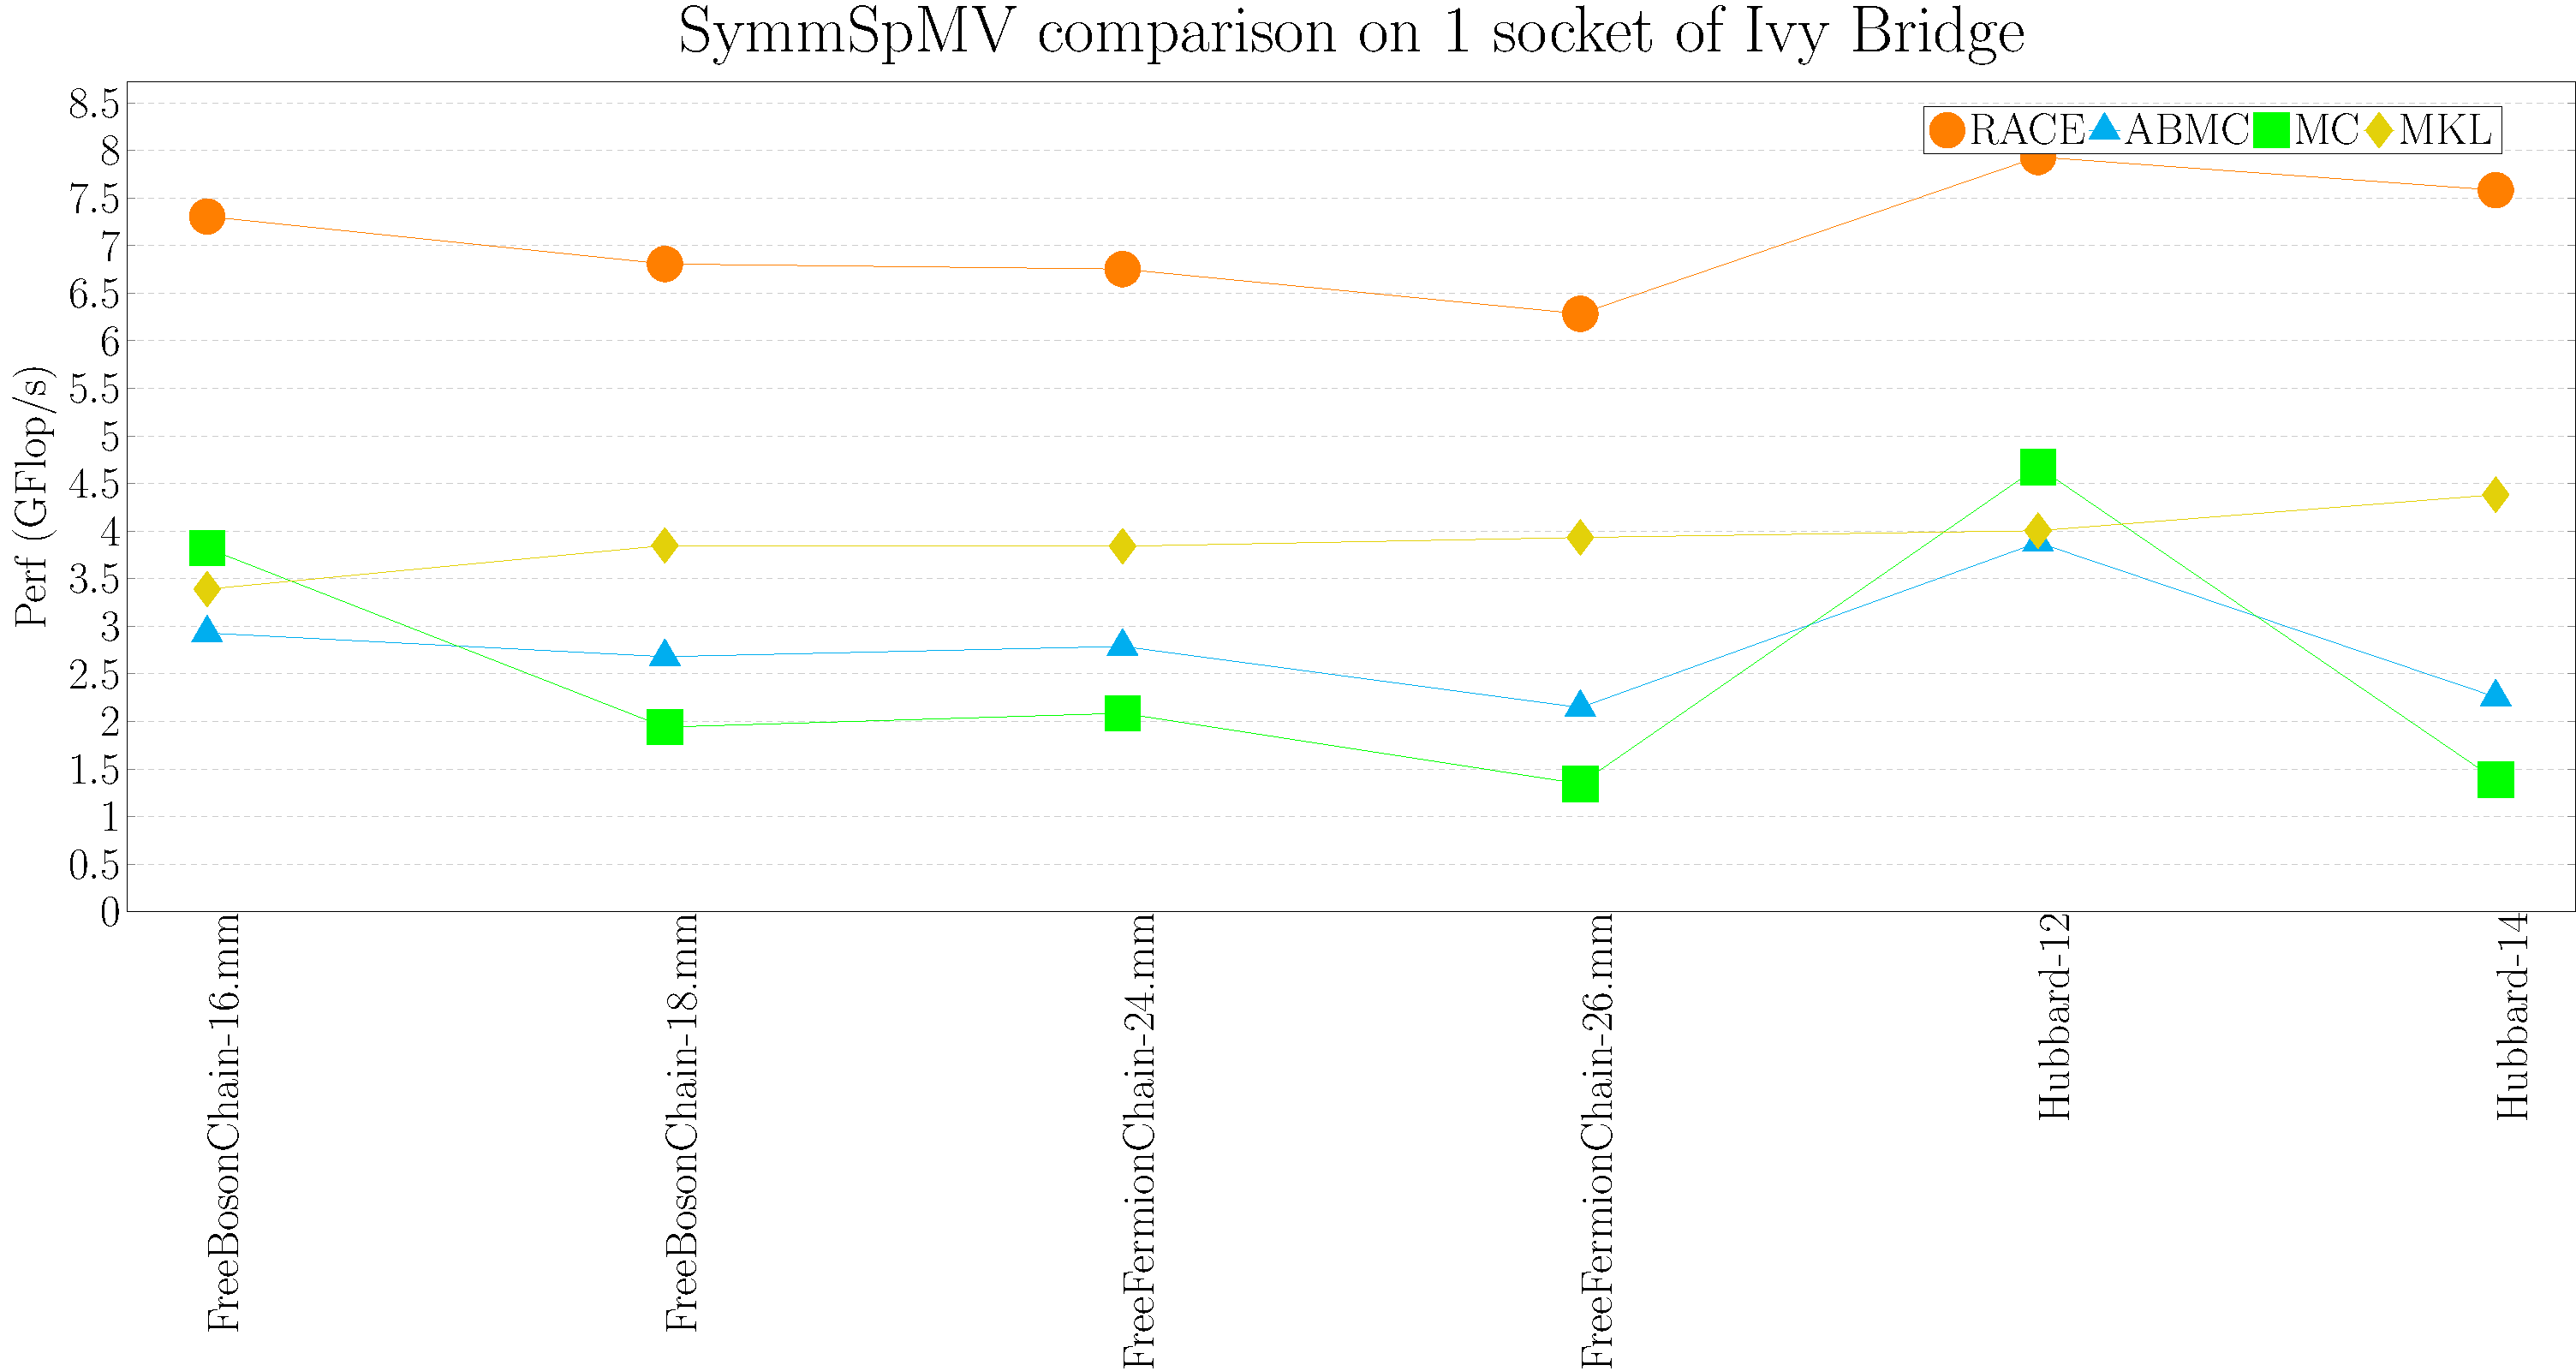
\includegraphics[width=0.48\textwidth, height=0.15\textheight]{pics/results/ivy/data_symm_spmv/plot_generator/perf_vs_mtx/ivy_scamac}}
	\hspace{1em}
	\subfloat[\acrshort{SymmSpMV} on 1 socket of \SKX]{\label{fig:symm_spmv_skx_scamac}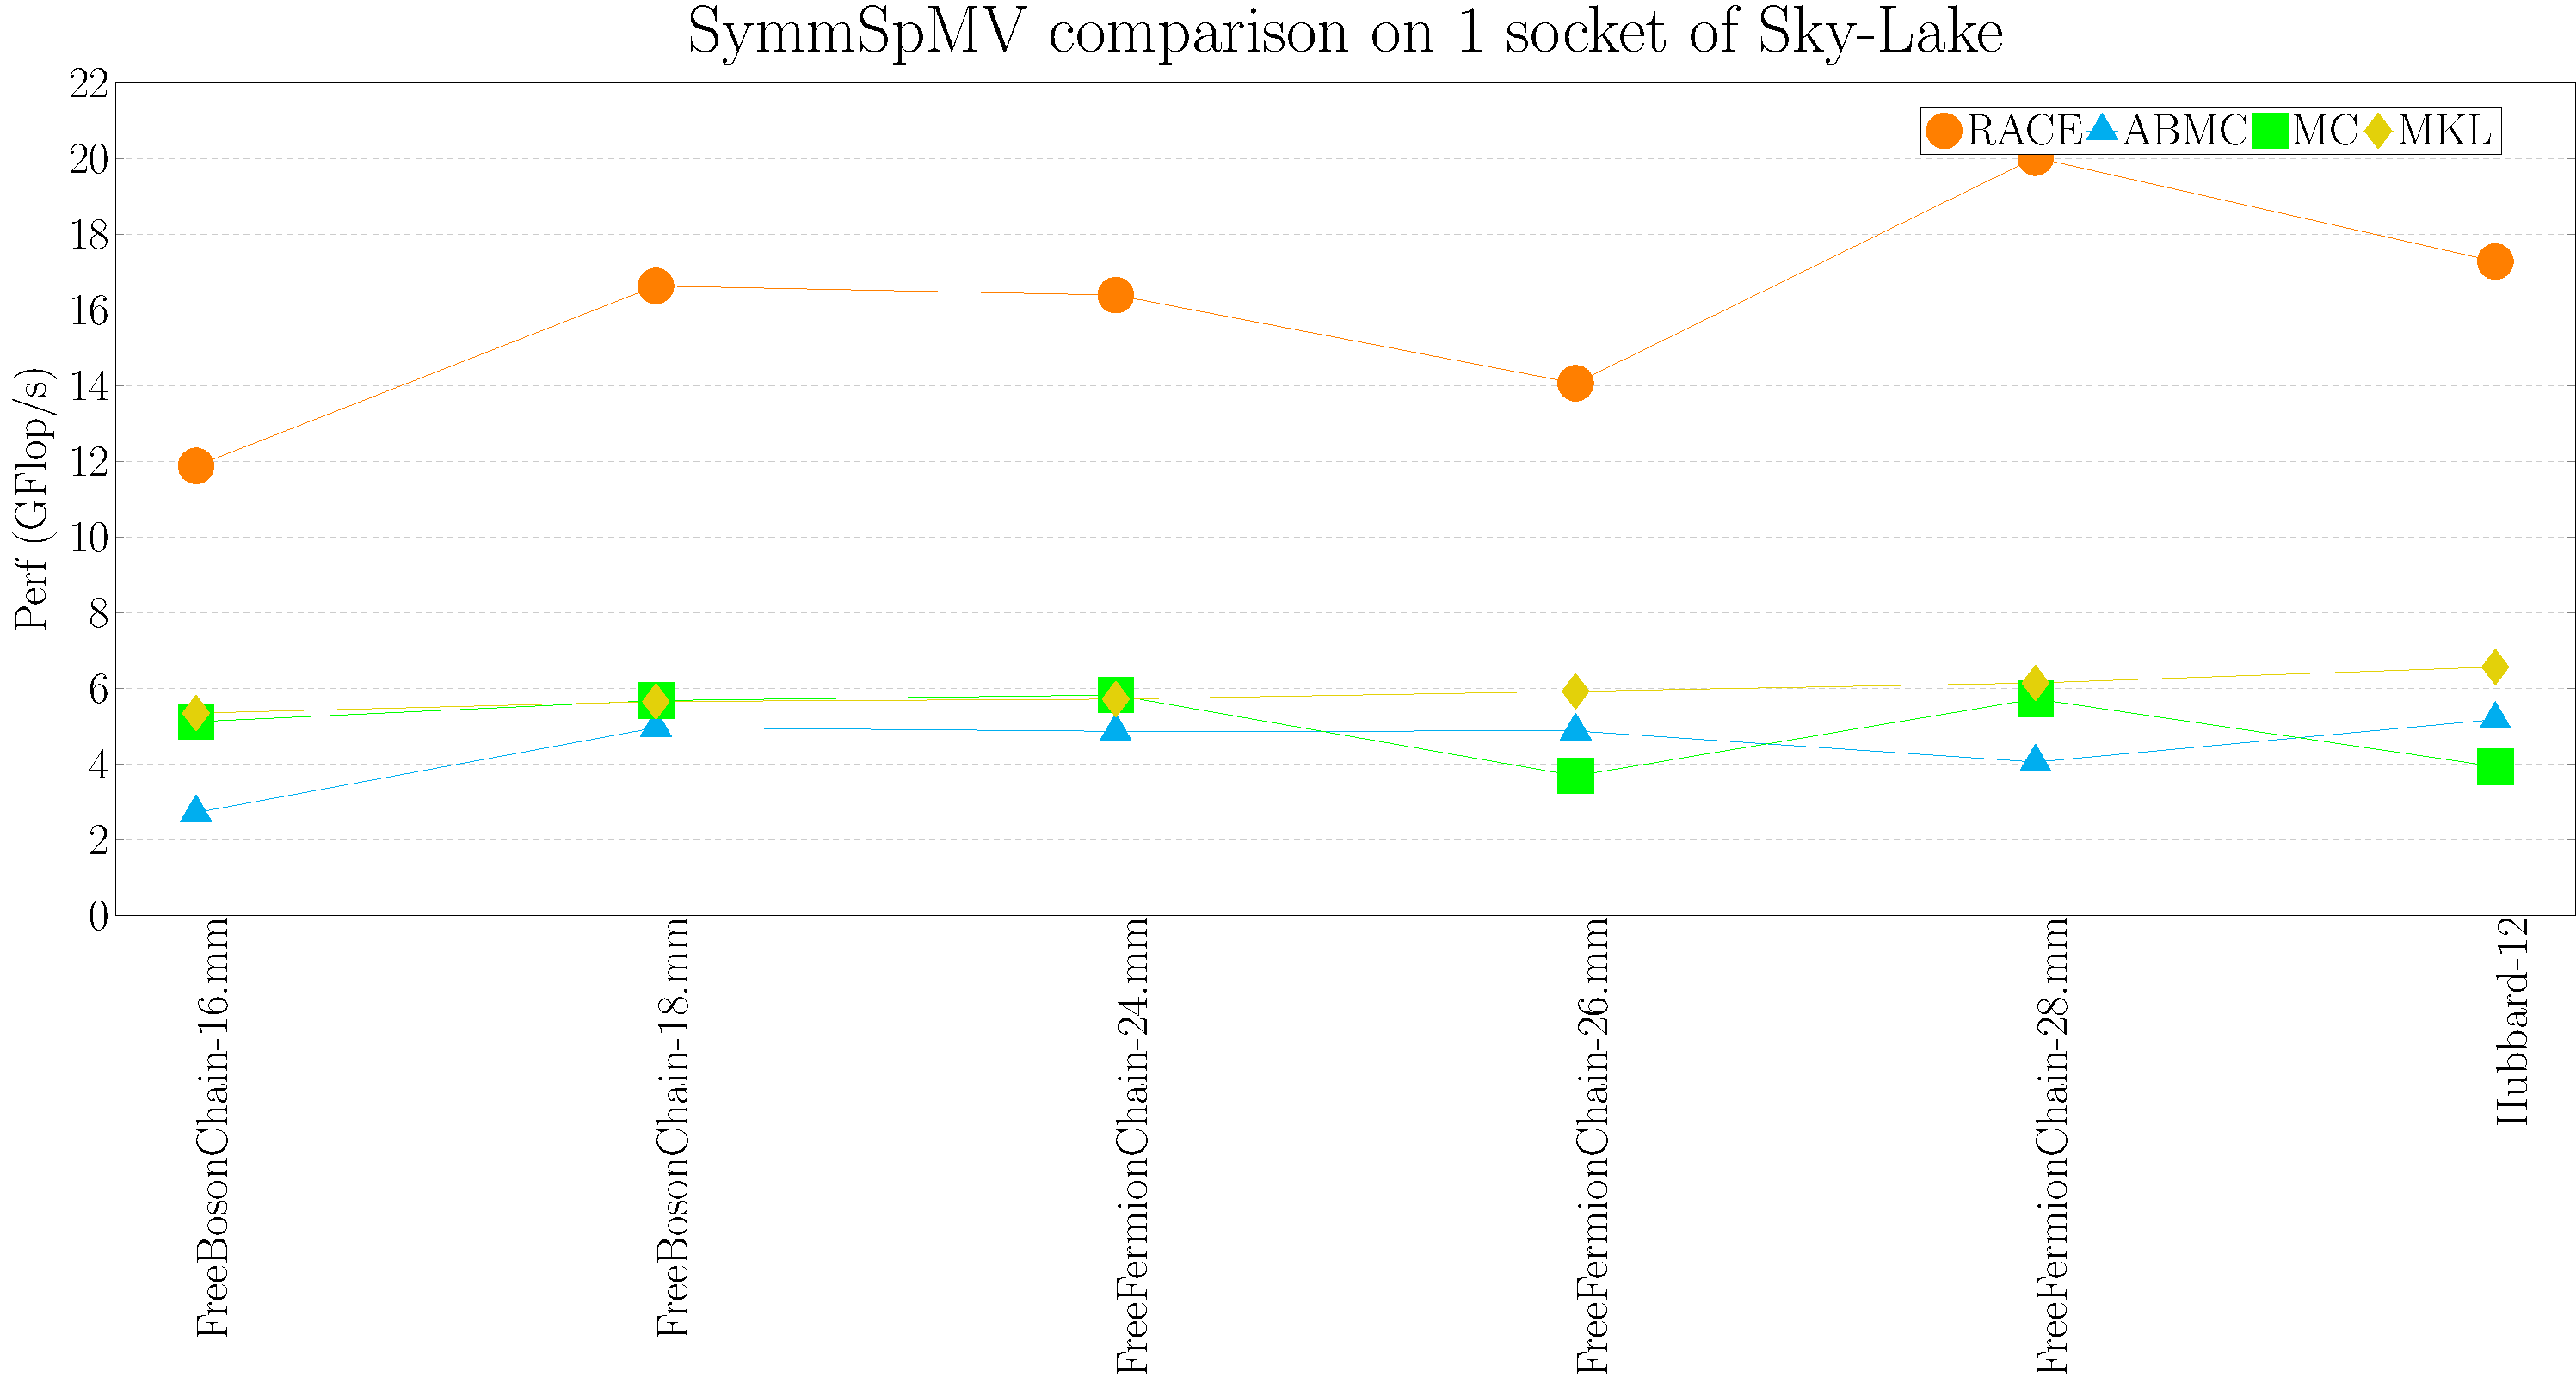
\includegraphics[width=0.48\textwidth, height=0.15\textheight]{pics/results/skx/data_symm_spmv/plot_generator/perf_vs_mtx/skx_scamac}}
	\caption{\acrshort{SymmSpMV} performance for SCAMAC matrices}
	\label{fig:symm_spmv_scamac}
\end{figure}

%\end{comment}

%\begin{figure}[thbp]
%	\centering
	%\subfloat[RACE performance compared to SpMV]{\label{fig:race_skx}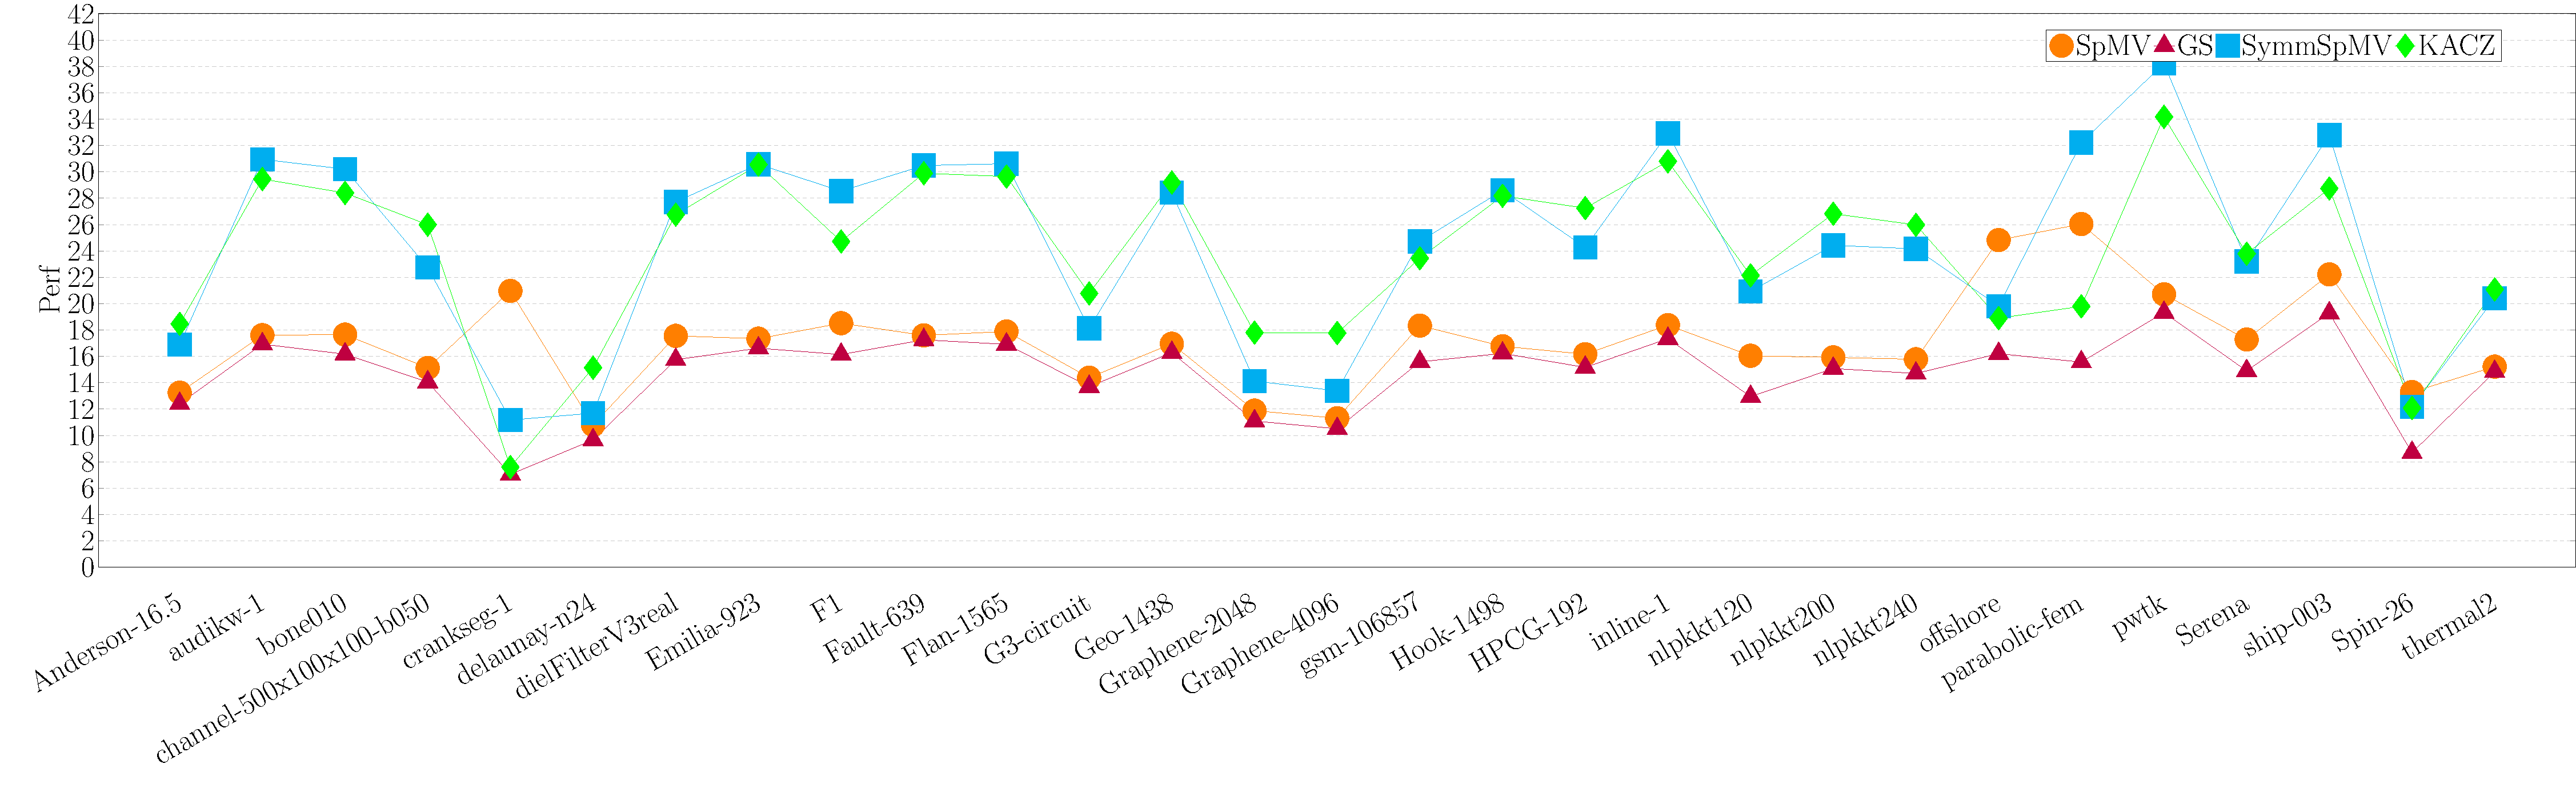
\includegraphics[width=0.45\textwidth, height=0.15\textheight]{pics/results/skx/race}}
	%\hspace{1.2em}
%	\subfloat[SymmSpMV Comparison]{\label{fig:symm_spmv_skx}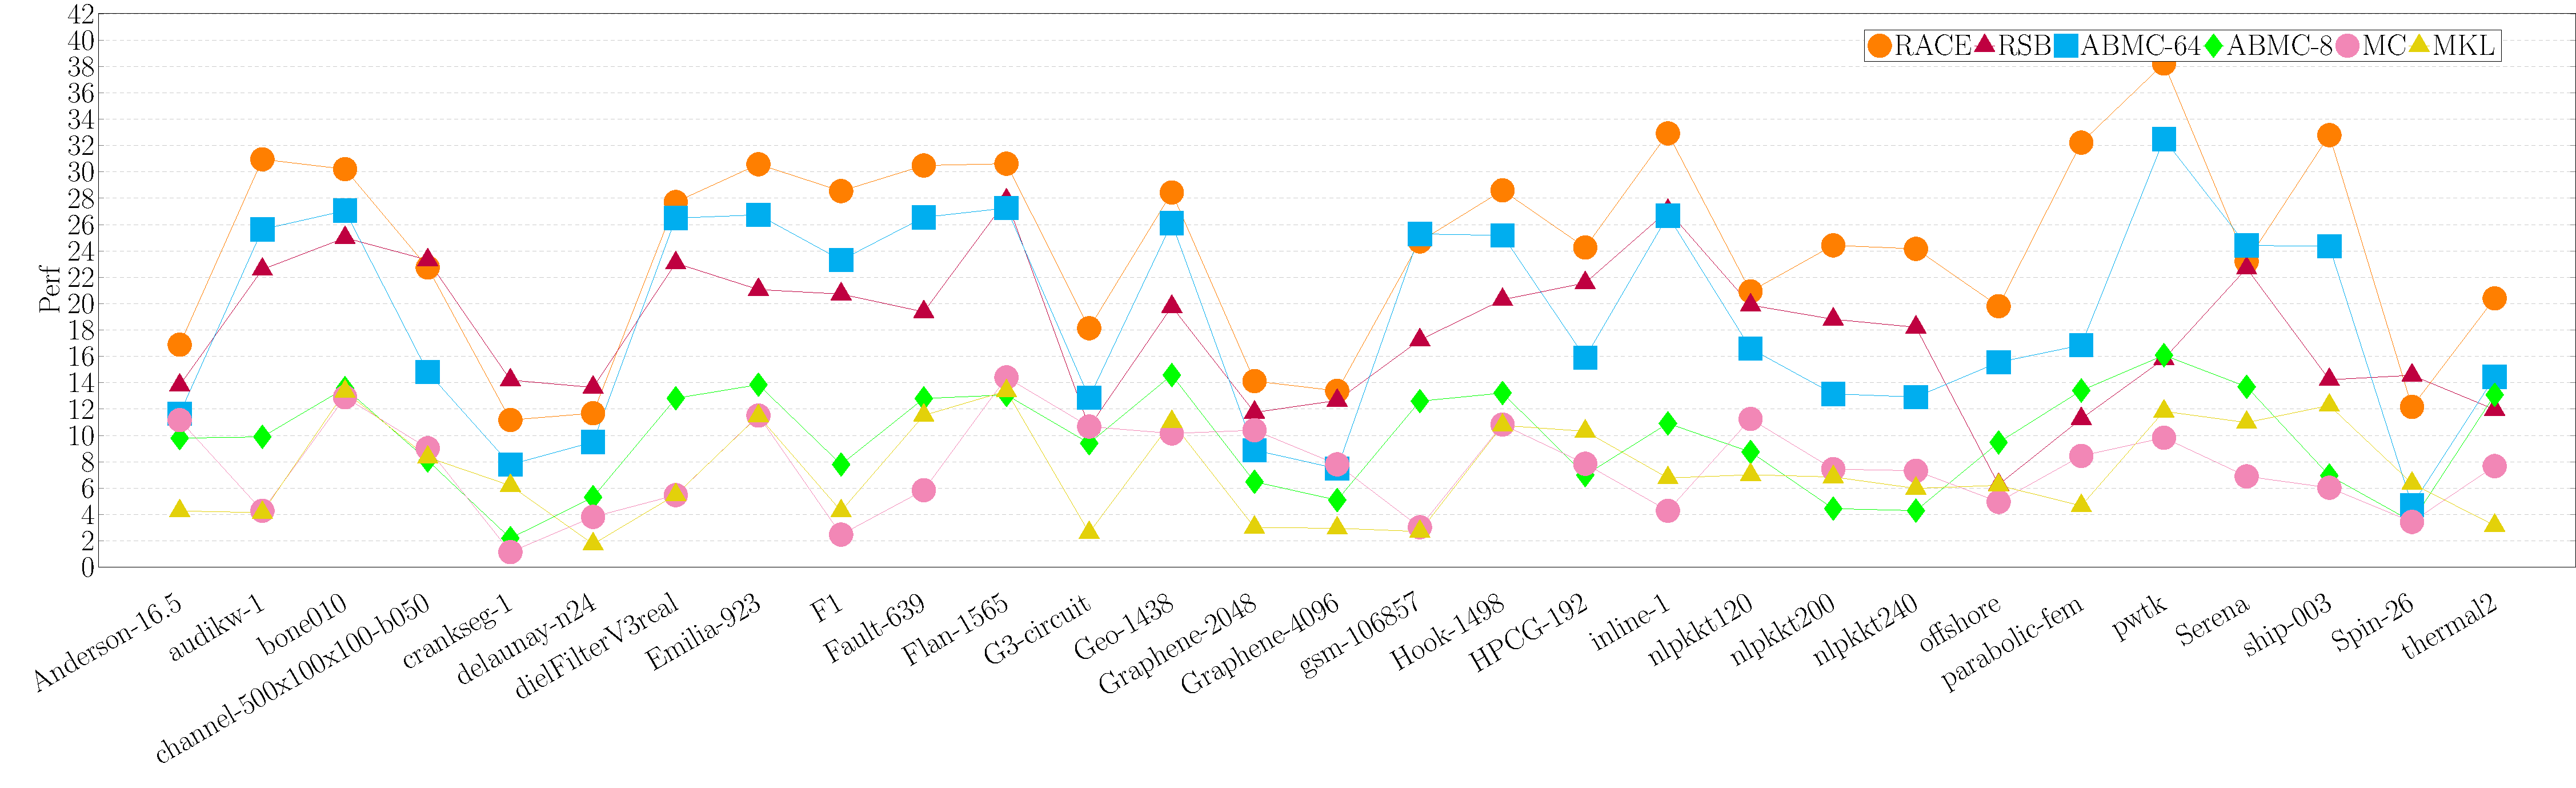
\includegraphics[width=0.45\textwidth, height=0.15\textheight]{pics/results/skx/symm_spmv}}
%	\hspace{1.2em}
	%\subfloat[GS Comparison]{\label{fig:gs_skx}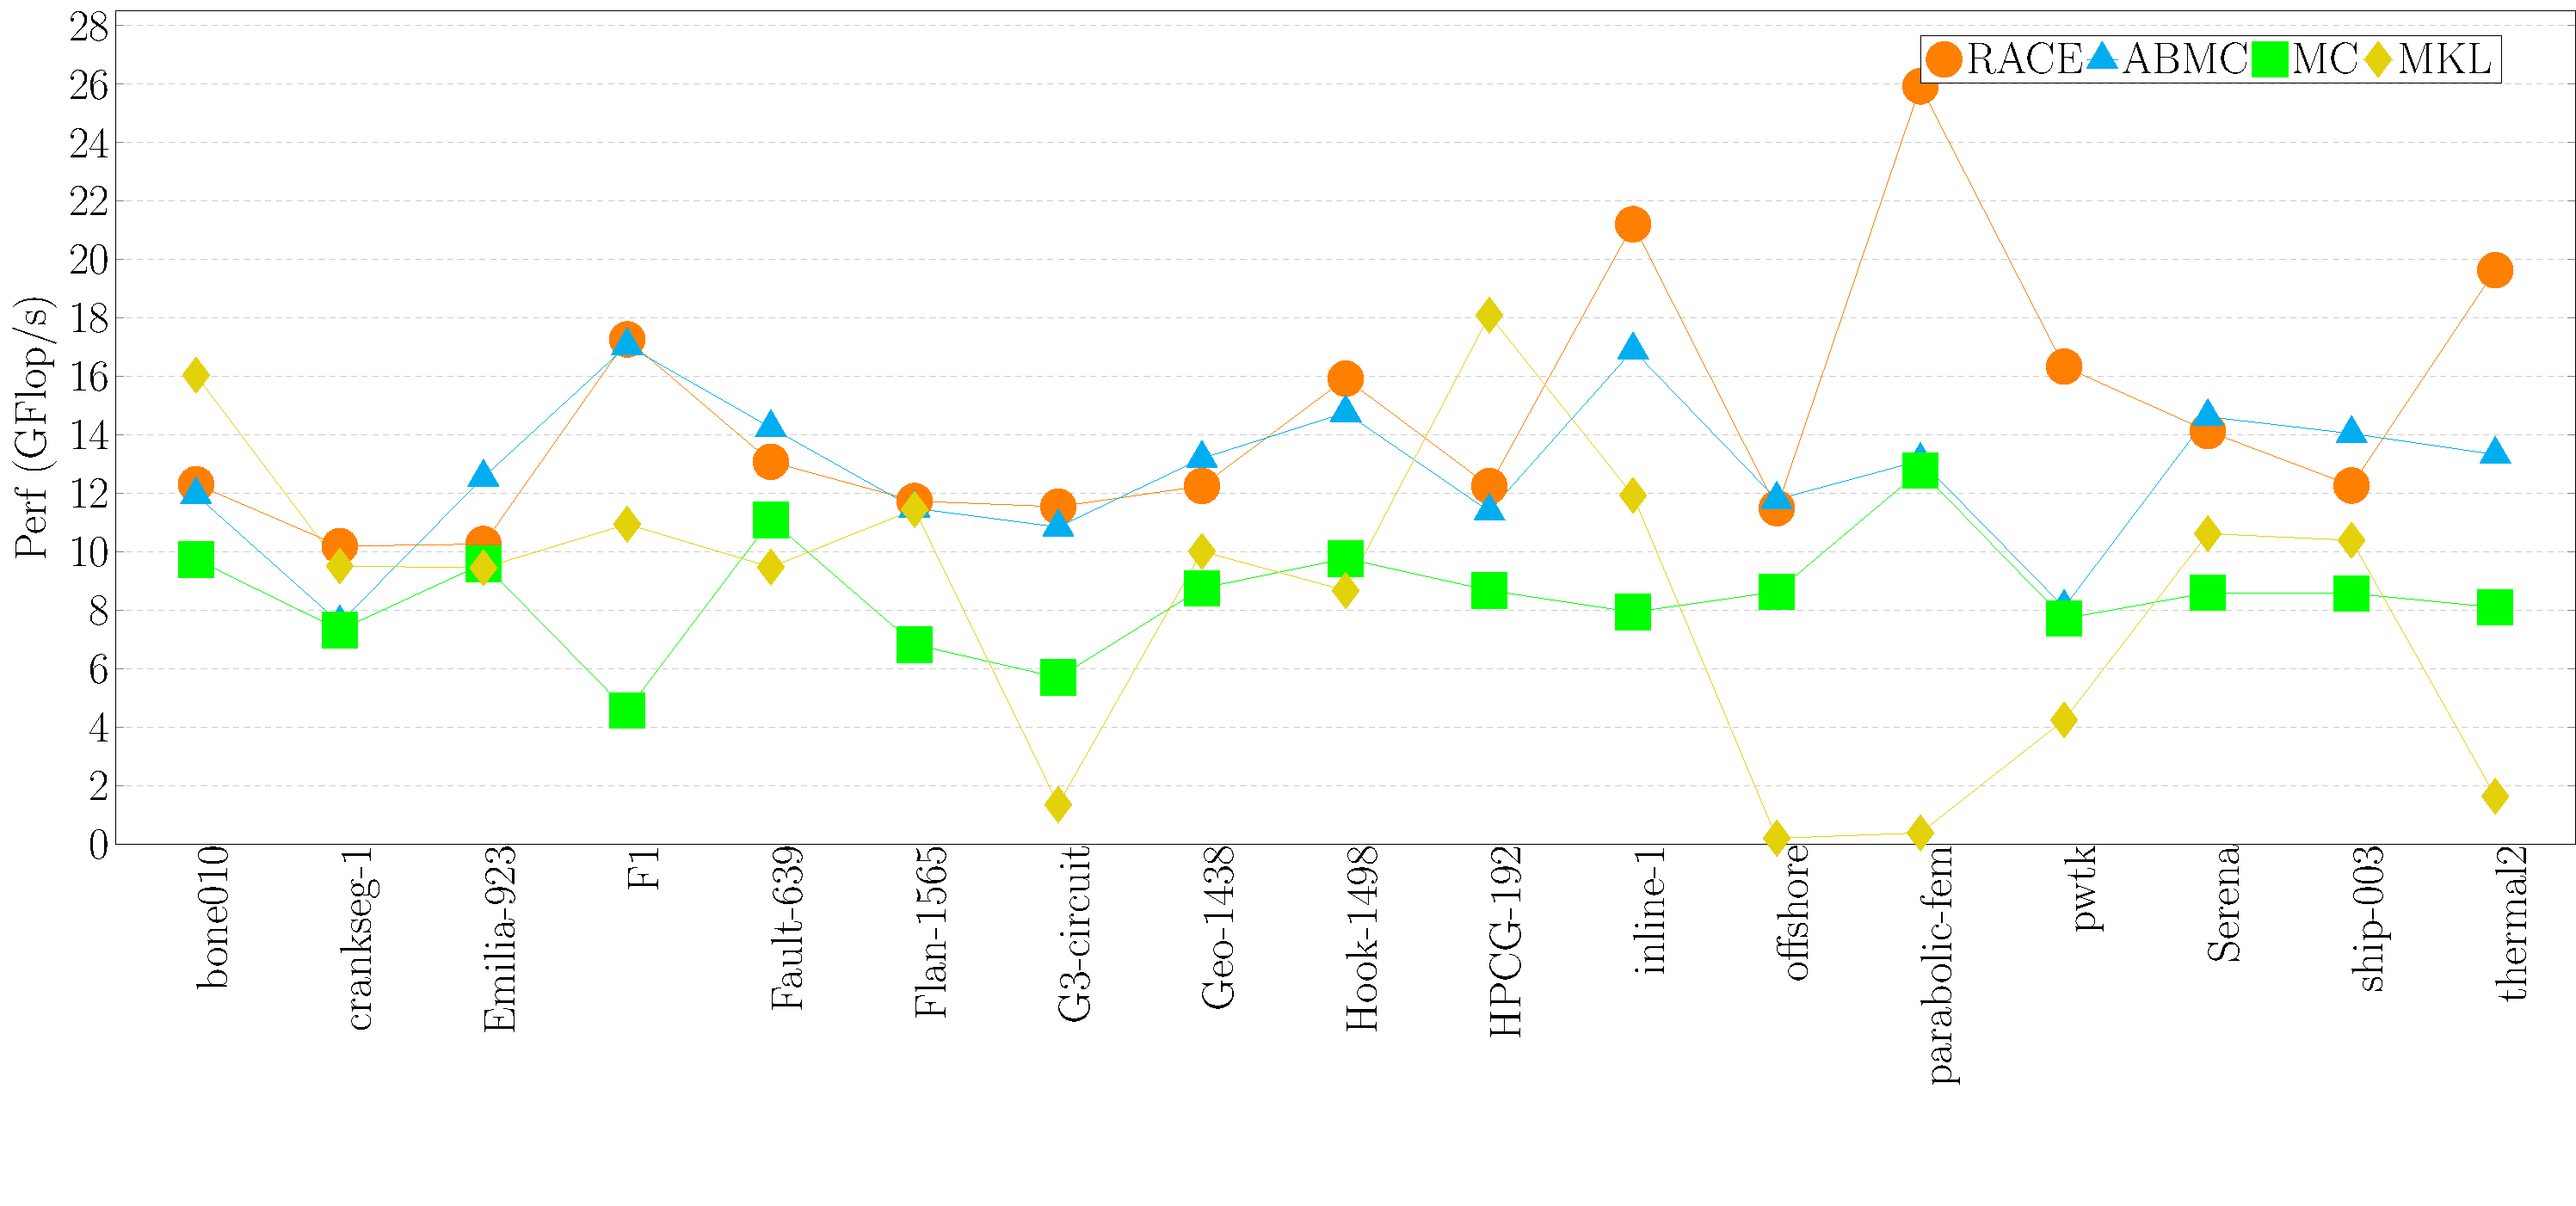
\includegraphics[width=0.45\textwidth, height=0.15\textheight]{pics/results/skx/gs}}
	%\hspace{1.2em}
%	\subfloat[KACZ Comparison]{\label{fig:kacz_skx}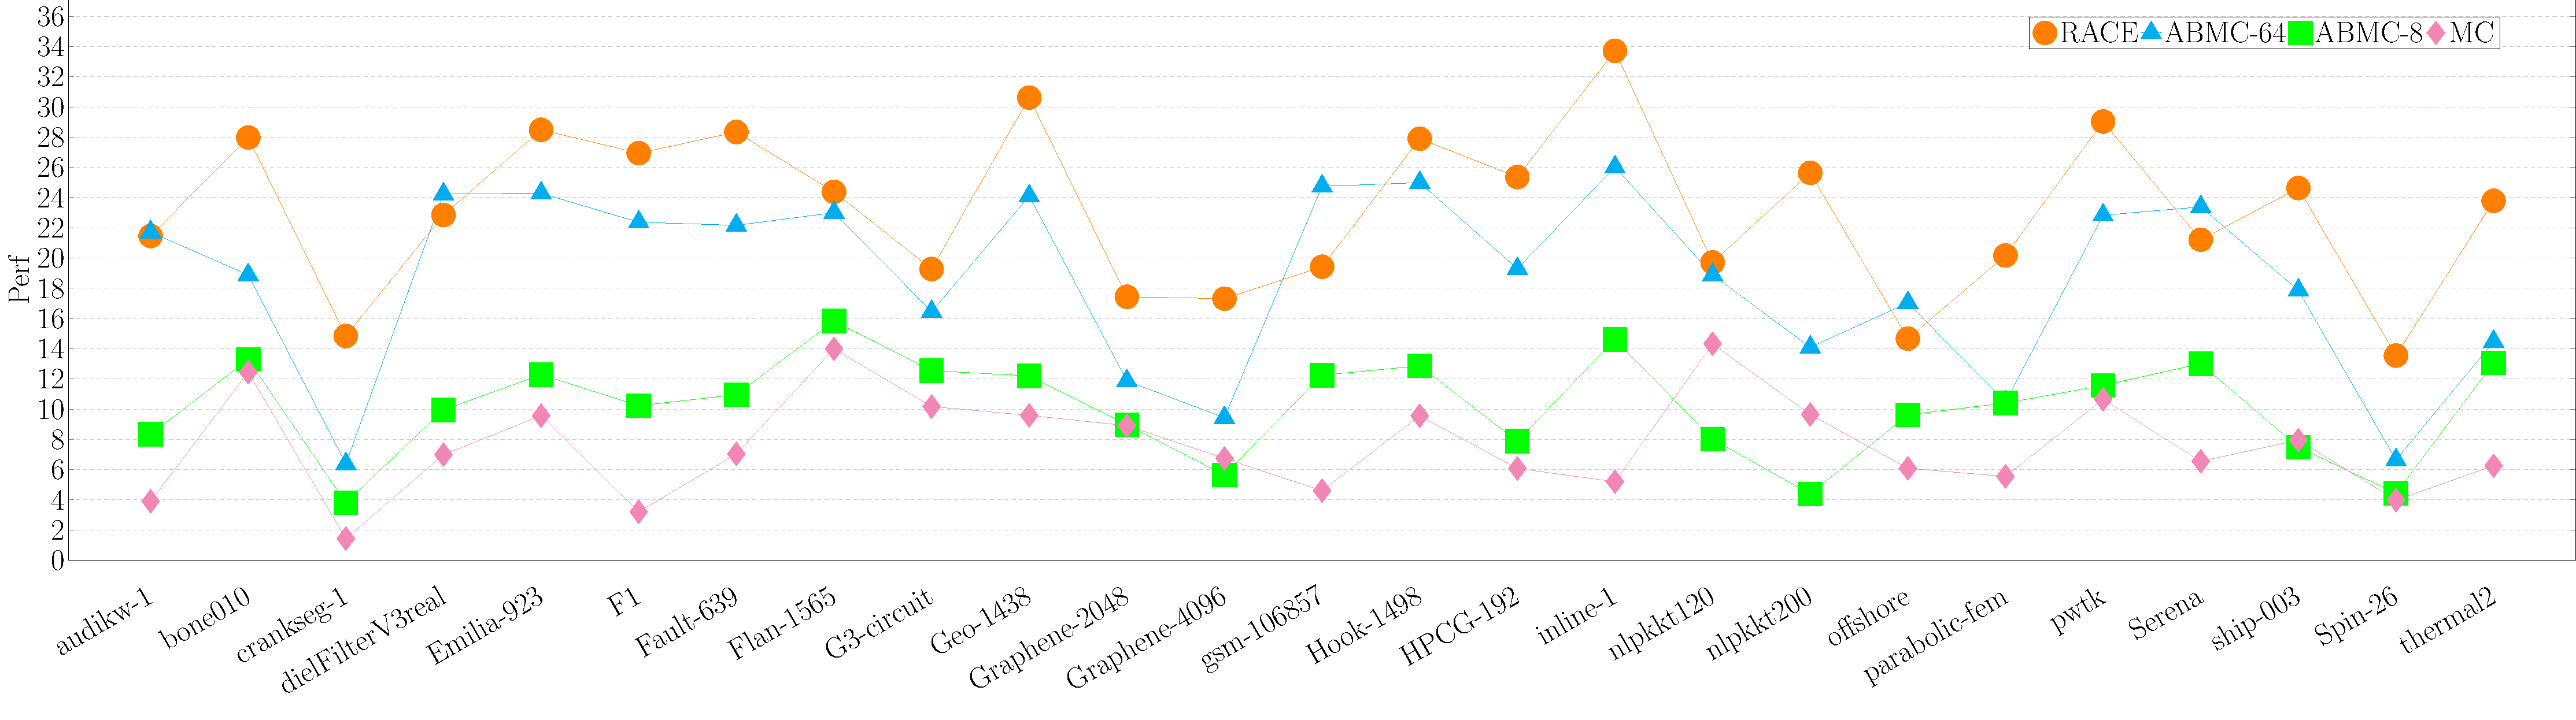
\includegraphics[width=0.45\textwidth, height=0.15\textheight]{pics/results/skx/kacz}}
%	\caption{Performance results on \SKX}
%	\label{fig:skx}
%\end{figure}

%\subsubsection{RACE performance}
%Here we plot the performance of \acrshort{SymmSpMV}, \GS and \KACZ with \acrshort{RACE} compared to \acrshort{SpMV}. \Cref{fig:race_ivy,fig:race_skx} will be used here. This is done for entire test matrices and all the hardwares. 

\subsubsection{Exact kernel}
Here we compare  \acrshort{RACE} with \acrshort{ABMC}, \acrshort{MC} and \acrshort{MKL} for \acrshort{SymmSpMV}. \Cref{fig:symm_spmv_ivy,fig:symm_spmv_skx} will be used. \COLPACK \cite{COLPACK} %TOD cite
was used for multicoloring (\acrshort{MC}). \METIS \cite{METIS}  was used for graph partitioning for \acrshort{ABMC}, and \COLPACK was used for coloring the hyper graph. The blocksize for \acrshort{ABMC} is chosen by doing parameter scan over 4 to 128 as shown by Iwashita \etal in \cite{ABMC}, and choosing the optimal one. Note that the time for this parameter search is not included in the performance results shown. 

\end{comment}


\subsubsection{Iterative kernel}

\begin{figure}[thbp]
	\centering
	\subfloat[1 socket \IVB] {\label{fig:derived_perf_kacz_ivb}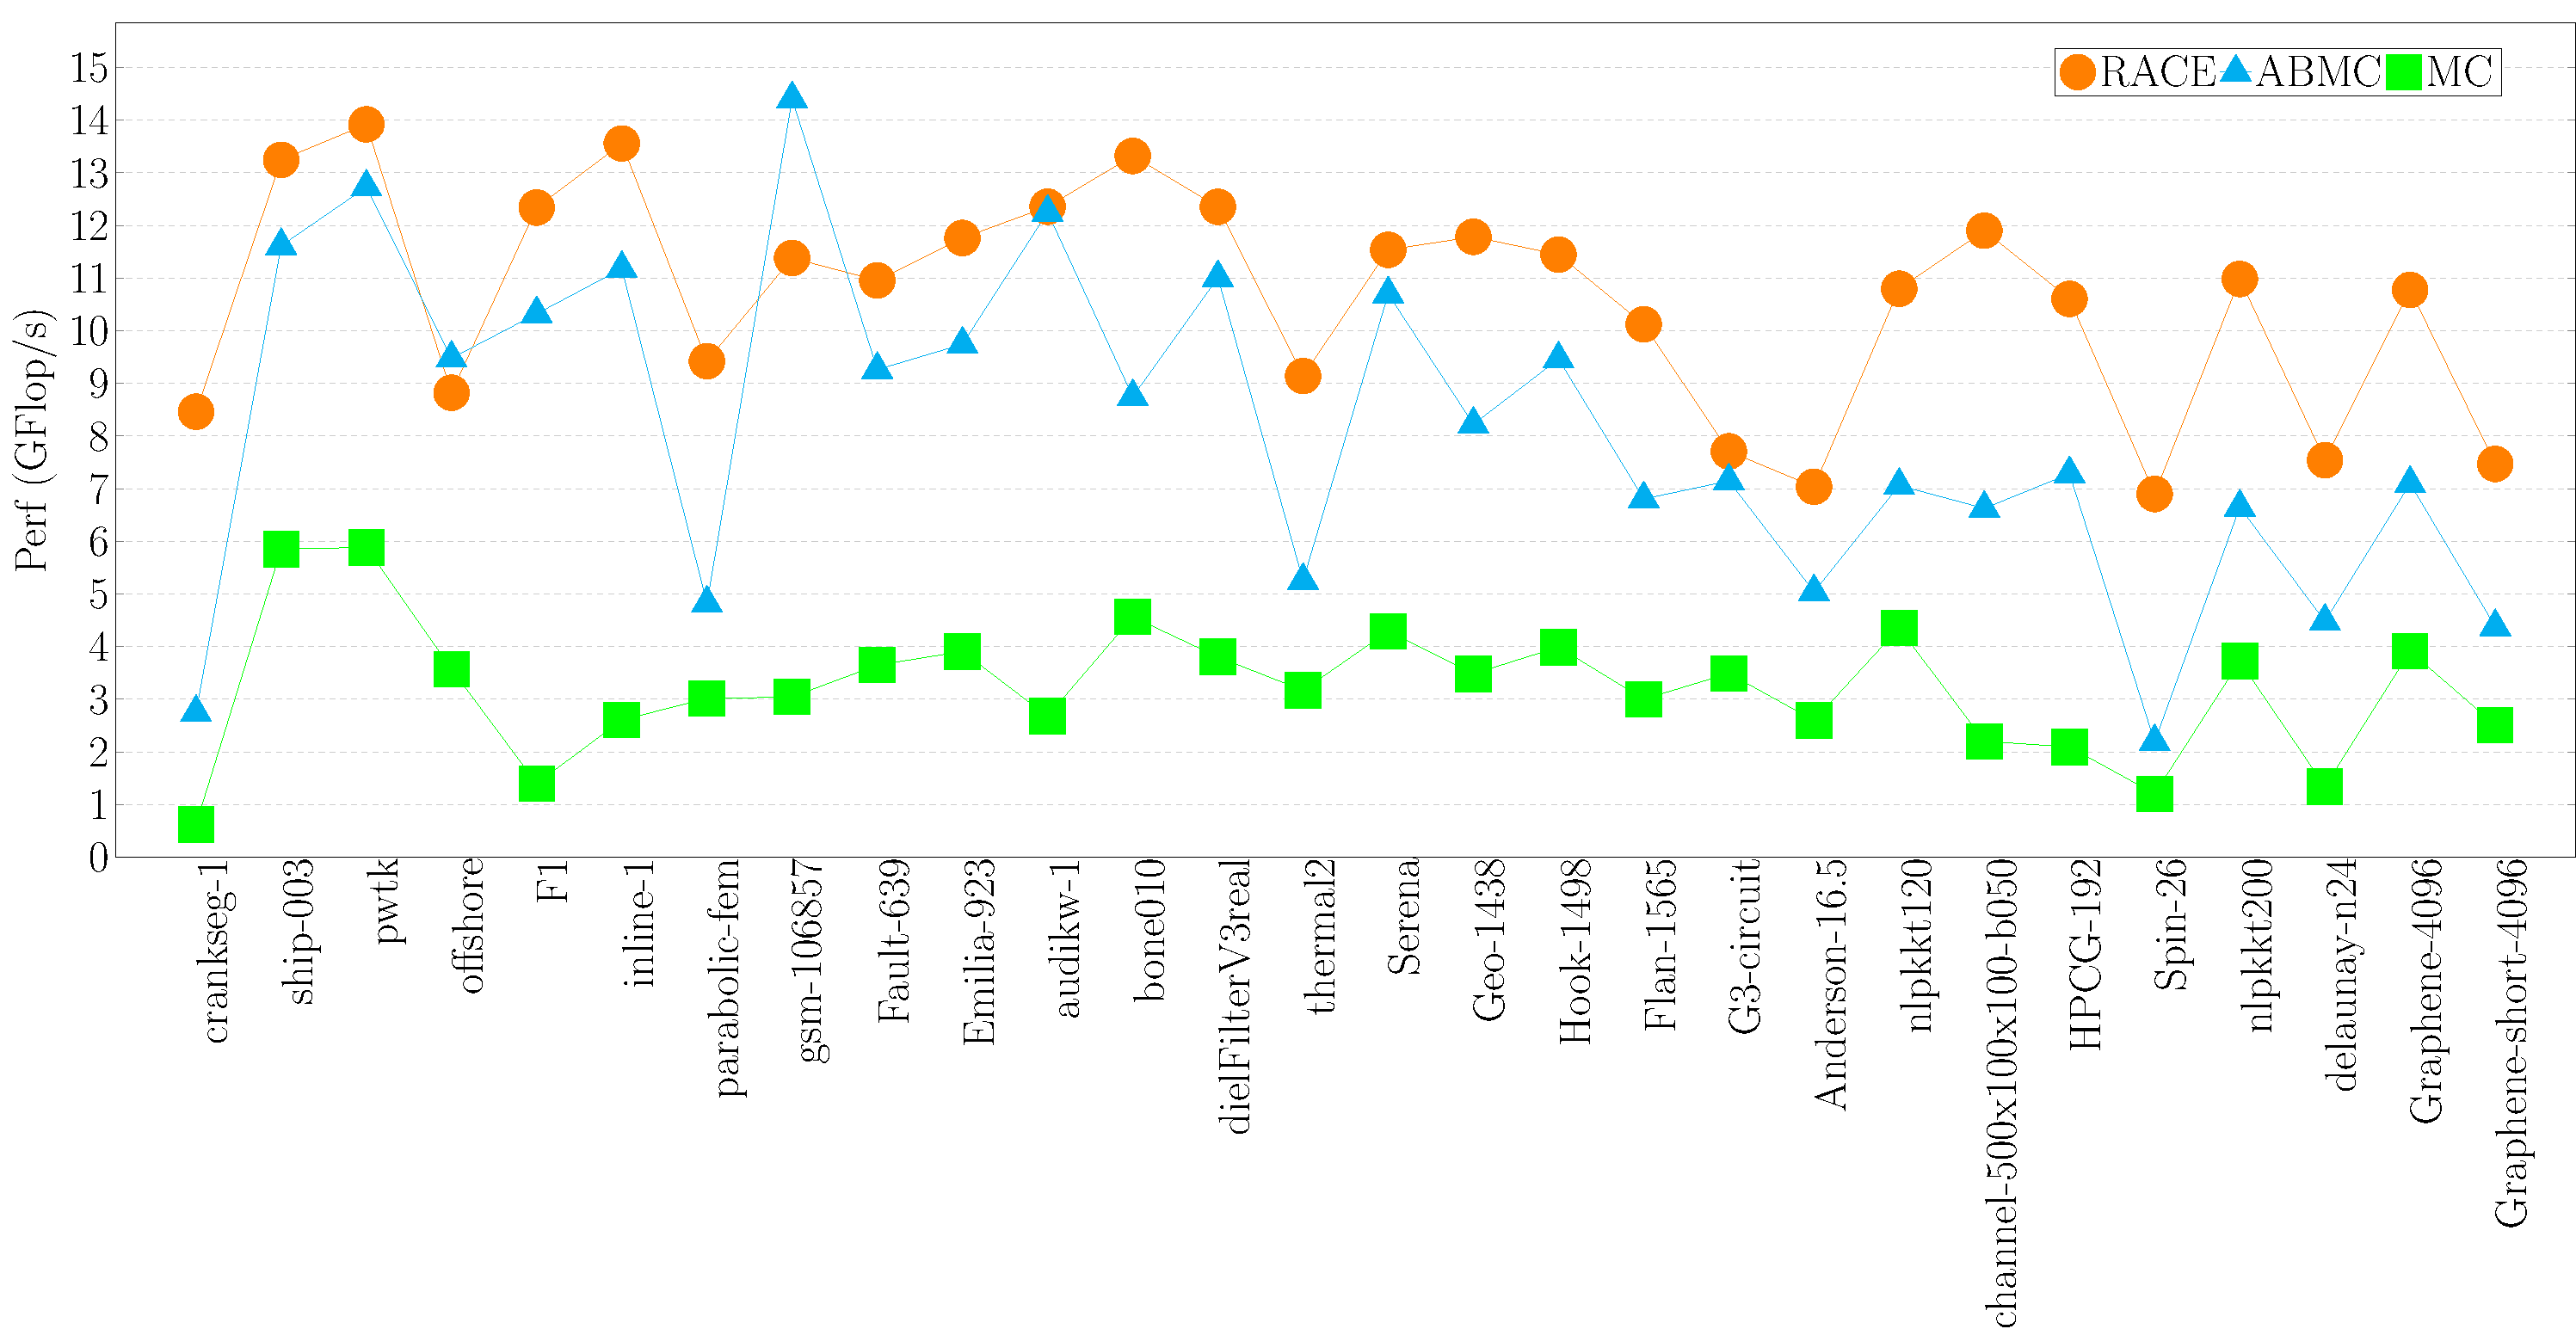
\includegraphics[width=0.85\textwidth, height=0.27\textheight]{pics/results/ivy/data_symm_kacz/plot_generator/derived_perf_vs_mtx/derived_perf}}
	\hspace{1em}
	\subfloat[1 socket \SKX] {\label{fig:derived_perf_kacz_skx}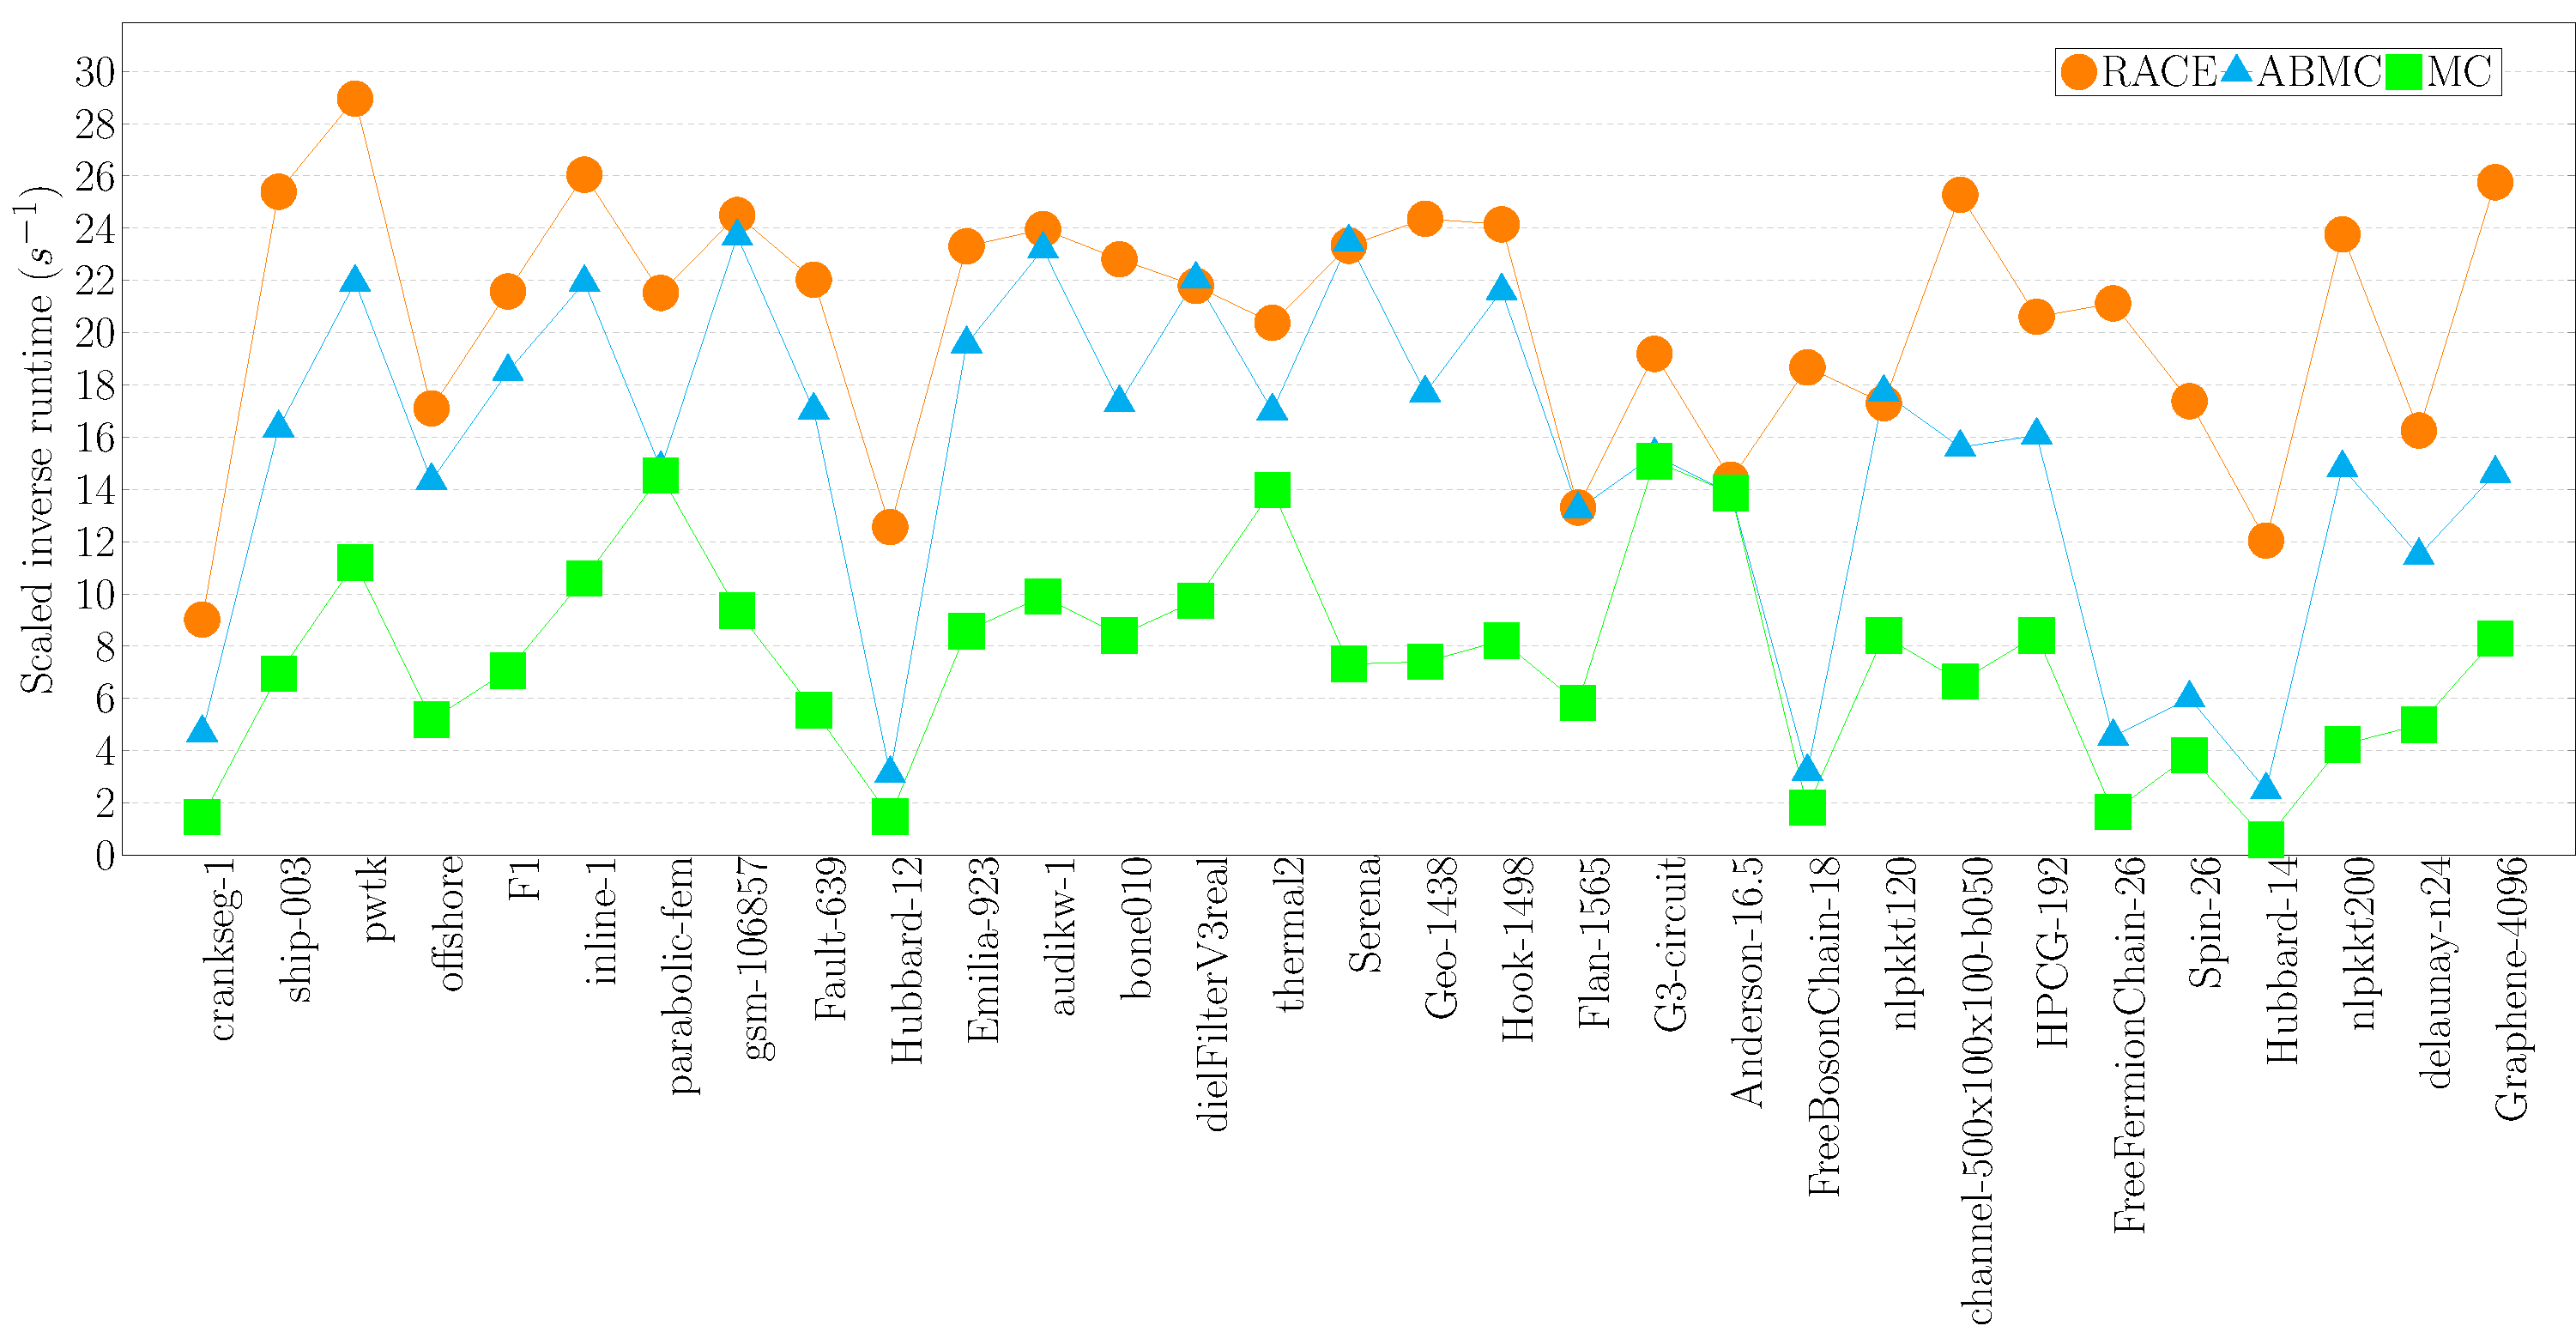
\includegraphics[width=0.85\textwidth, height=0.27\textheight]{pics/results/skx/data_symm_kacz/plot_generator/derived_perf_vs_mtx/derived_perf}}
	\caption{\acrshort{SymmKACZ} inverse runtime (scaled)}
	\label{fig:symmkacz_dp}
\end{figure}

\begin{figure}[thbp]
	\centering
	\subfloat[Plain performance] {\label{fig:perf_kacz_ivb}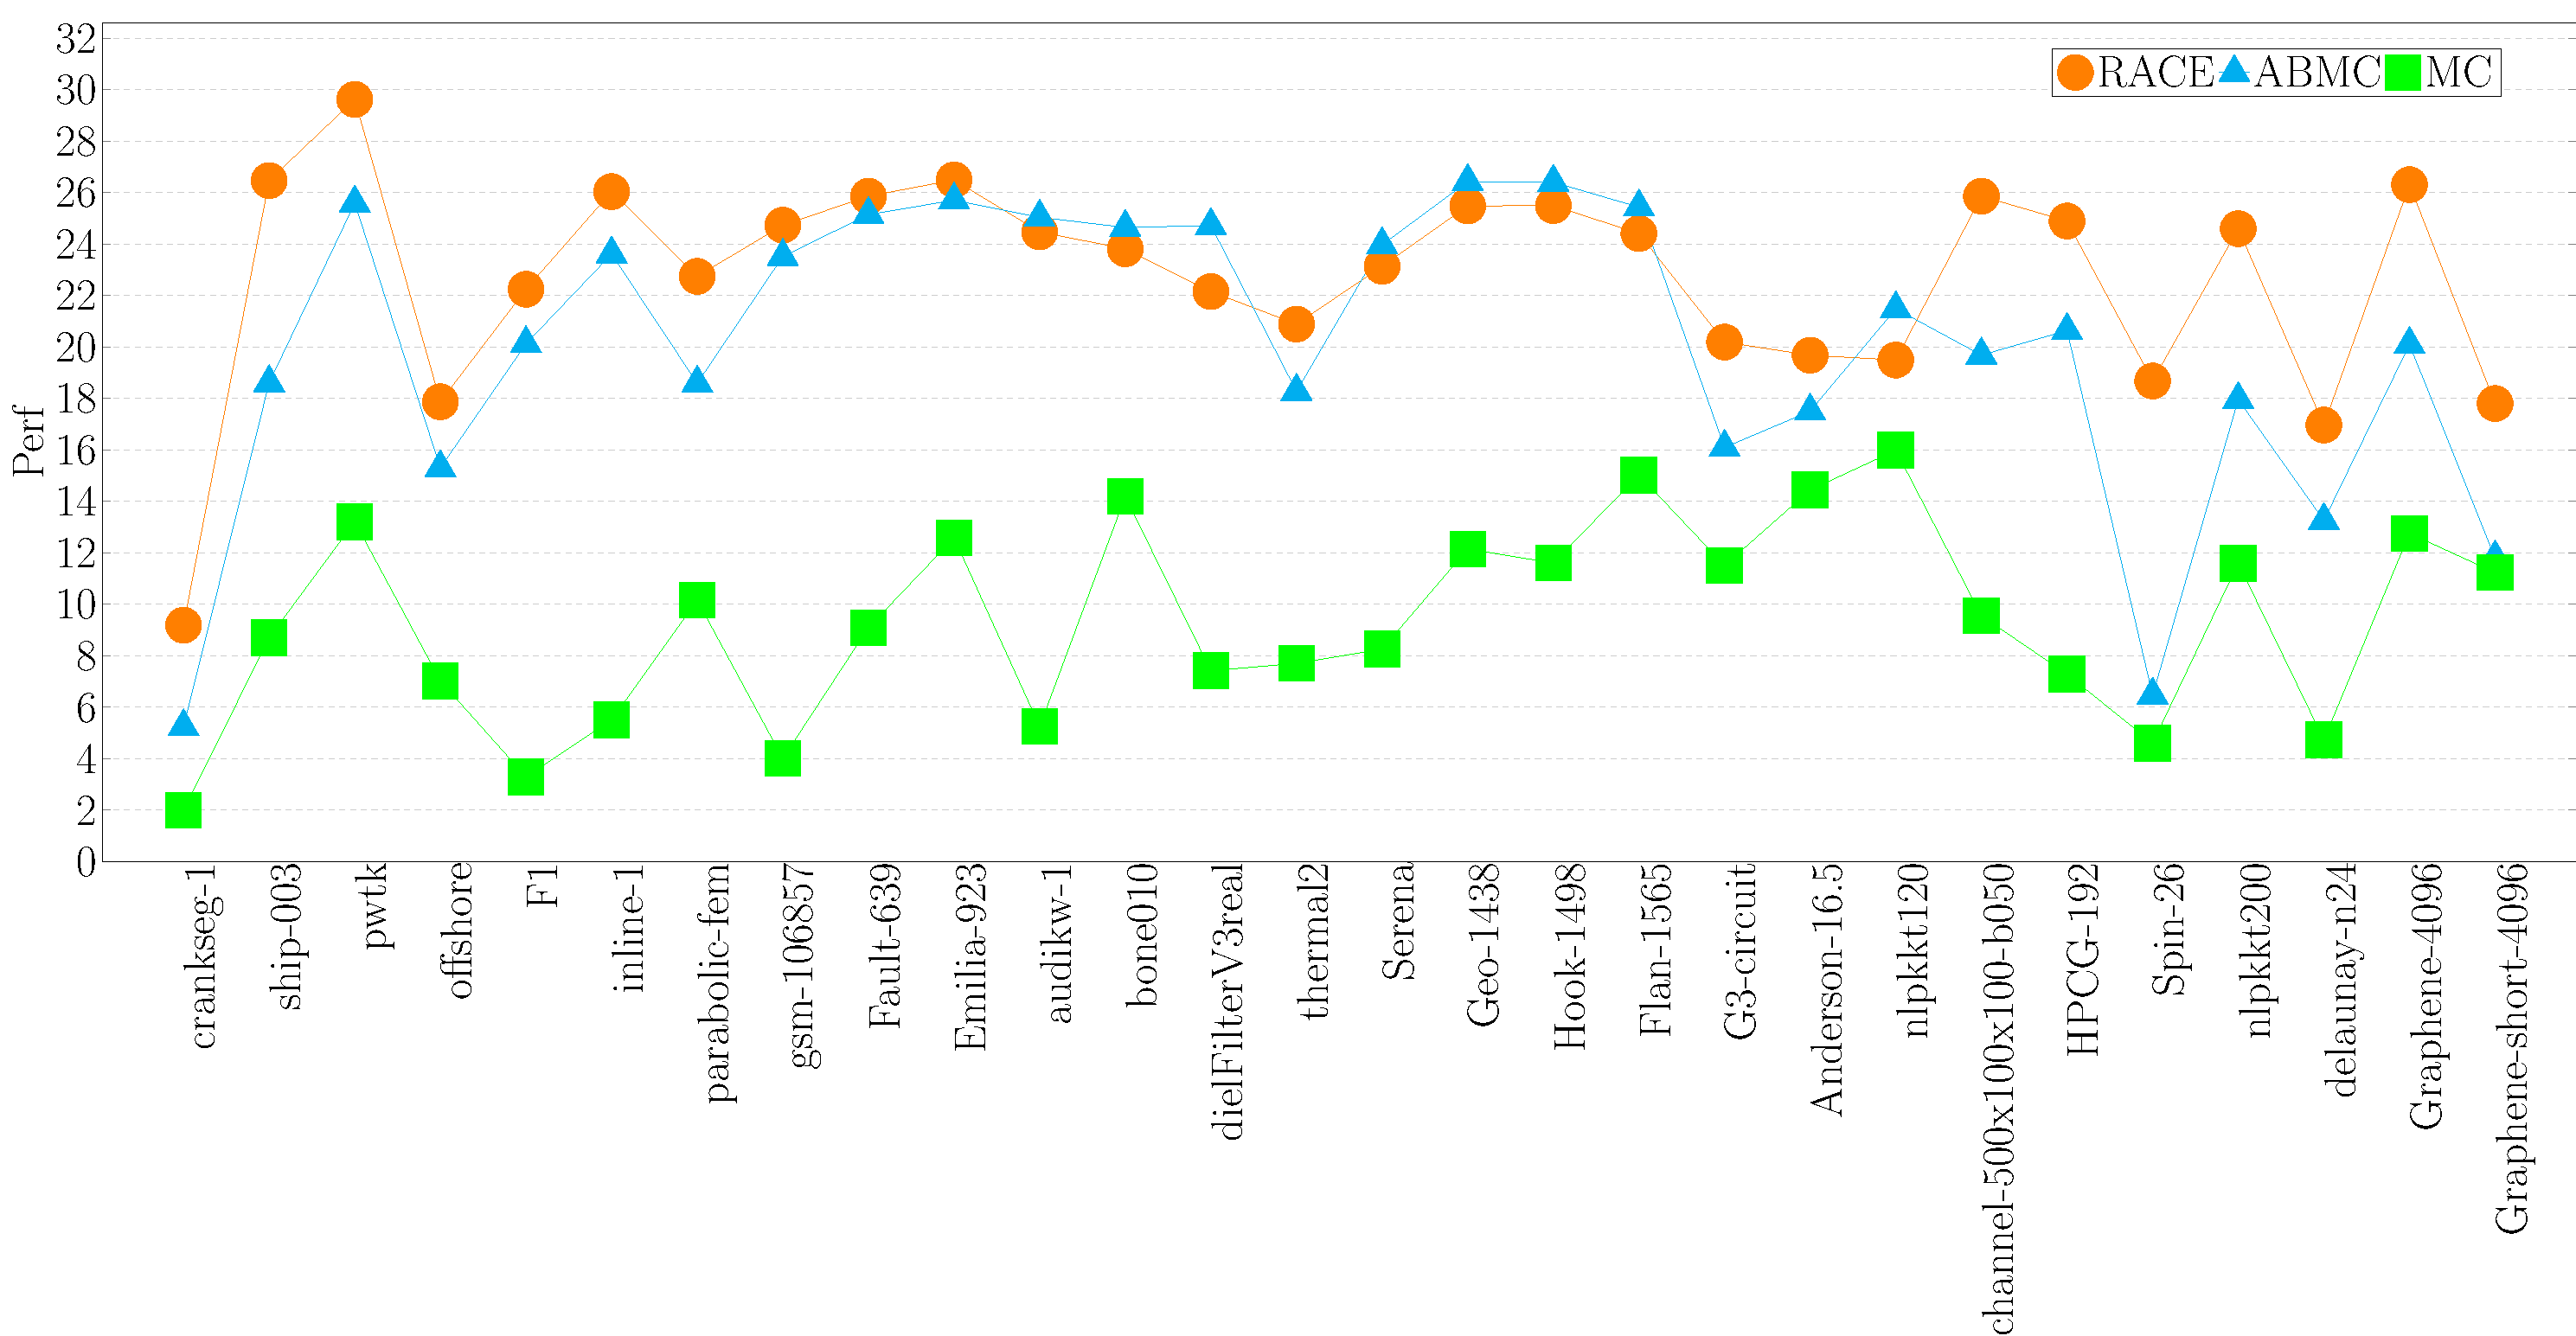
\includegraphics[width=0.85\textwidth, height=0.27\textheight]{pics/results/skx/data_symm_kacz/plot_generator/perf_vs_mtx/perf}}
	\hspace{1em}
	\subfloat[Iterations compared to serial \acrshort{SymmKACZ} kernel, note that for Hubbard-12, FreeBosonChain-18, FreeFermionChain-26 and Hubbard-14 the iteration count (y-axis) has to be multiplied by a factor of 50] {\label{fig:iter_kacz_skx}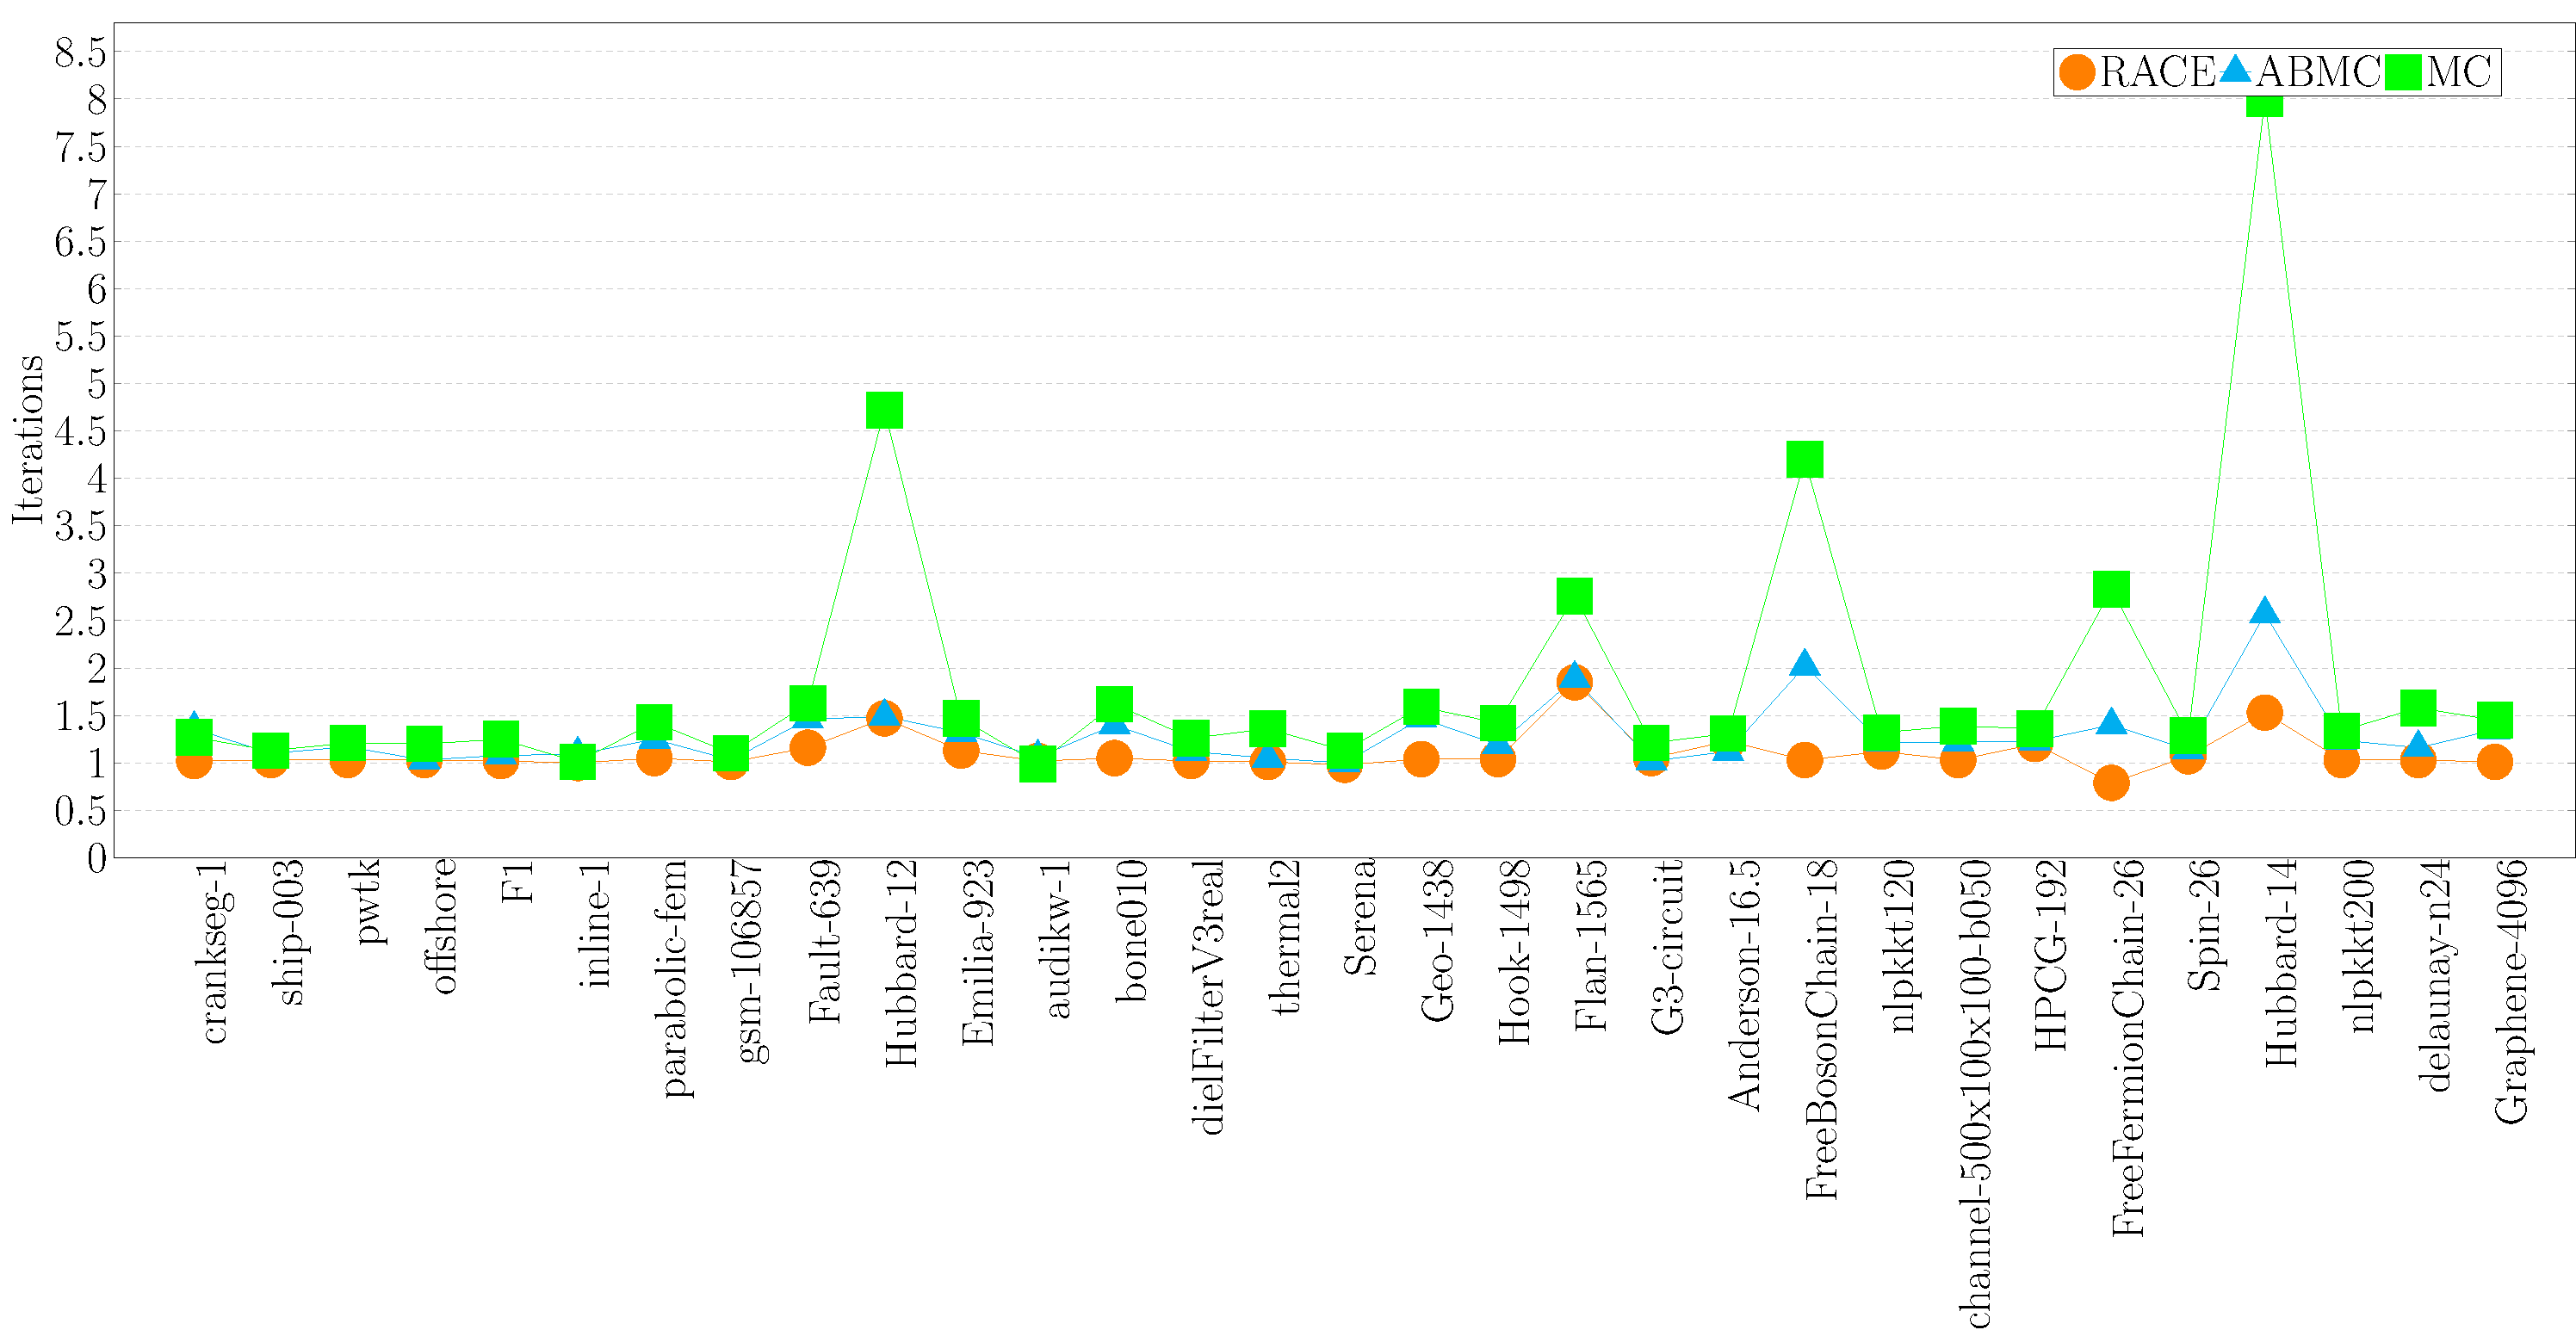
\includegraphics[width=0.85\textwidth, height=0.27\textheight]{pics/results/skx/data_symm_kacz/plot_generator/iter_vs_mtx/iter}}
	\caption{\acrshort{SymmKACZ} convergence study on \SKX}
	\label{fig:symmkacz_convergence}
\end{figure}
Here we compare  \acrshort{RACE} with \acrshort{ABMC} and \acrshort{MC} for \acrshort{SymmKACZ} kernel. Inverse runtime of \acrshort{SymmKACZ} kernel is shown in \cref{fig:symmkacz_dp}.

 Since each of the matrix reordering changes convergence of the kernel, it is necessary here to also study the convergence behavior. \Cref{fig:symmkacz_convergence} shows the plain performance and iterations required on \SKX (20 threads) architecture.

Note that matrices only compatible with the \acrshort{KACZ} solvers are shown in performance results.

% The exact implementation of \acrshort{MKL} for \SYMMGS is not explicitly stated and is not published. But due to the property of the solver having same convergence as serial case we believe level-scheduling is used. The usage of same kernels in Intel's implementation of HPCG benchmark where the usage of level-scheduling has been stated \cite{Park_HPCG} leads to more confidence in our assumption.



\subsubsection{Comparison with tailored data format}
Comparison of \acrshort{RACE} with \acrshort{RSB} data format. Note \acrshort{RSB} is pre-processed with \acrshort{RCM}, which improves its performance for some cases. \Cref{fig:race_vs_rsb_ivy,fig:race_vs_rsb_skx} shows this comparison.

\begin{figure}[thbp]
	\centering
	\subfloat[Comparison of \acrshort{RACE} with \acrshort{RSB} on \IVB] {\label{fig:race_vs_rsb_ivy}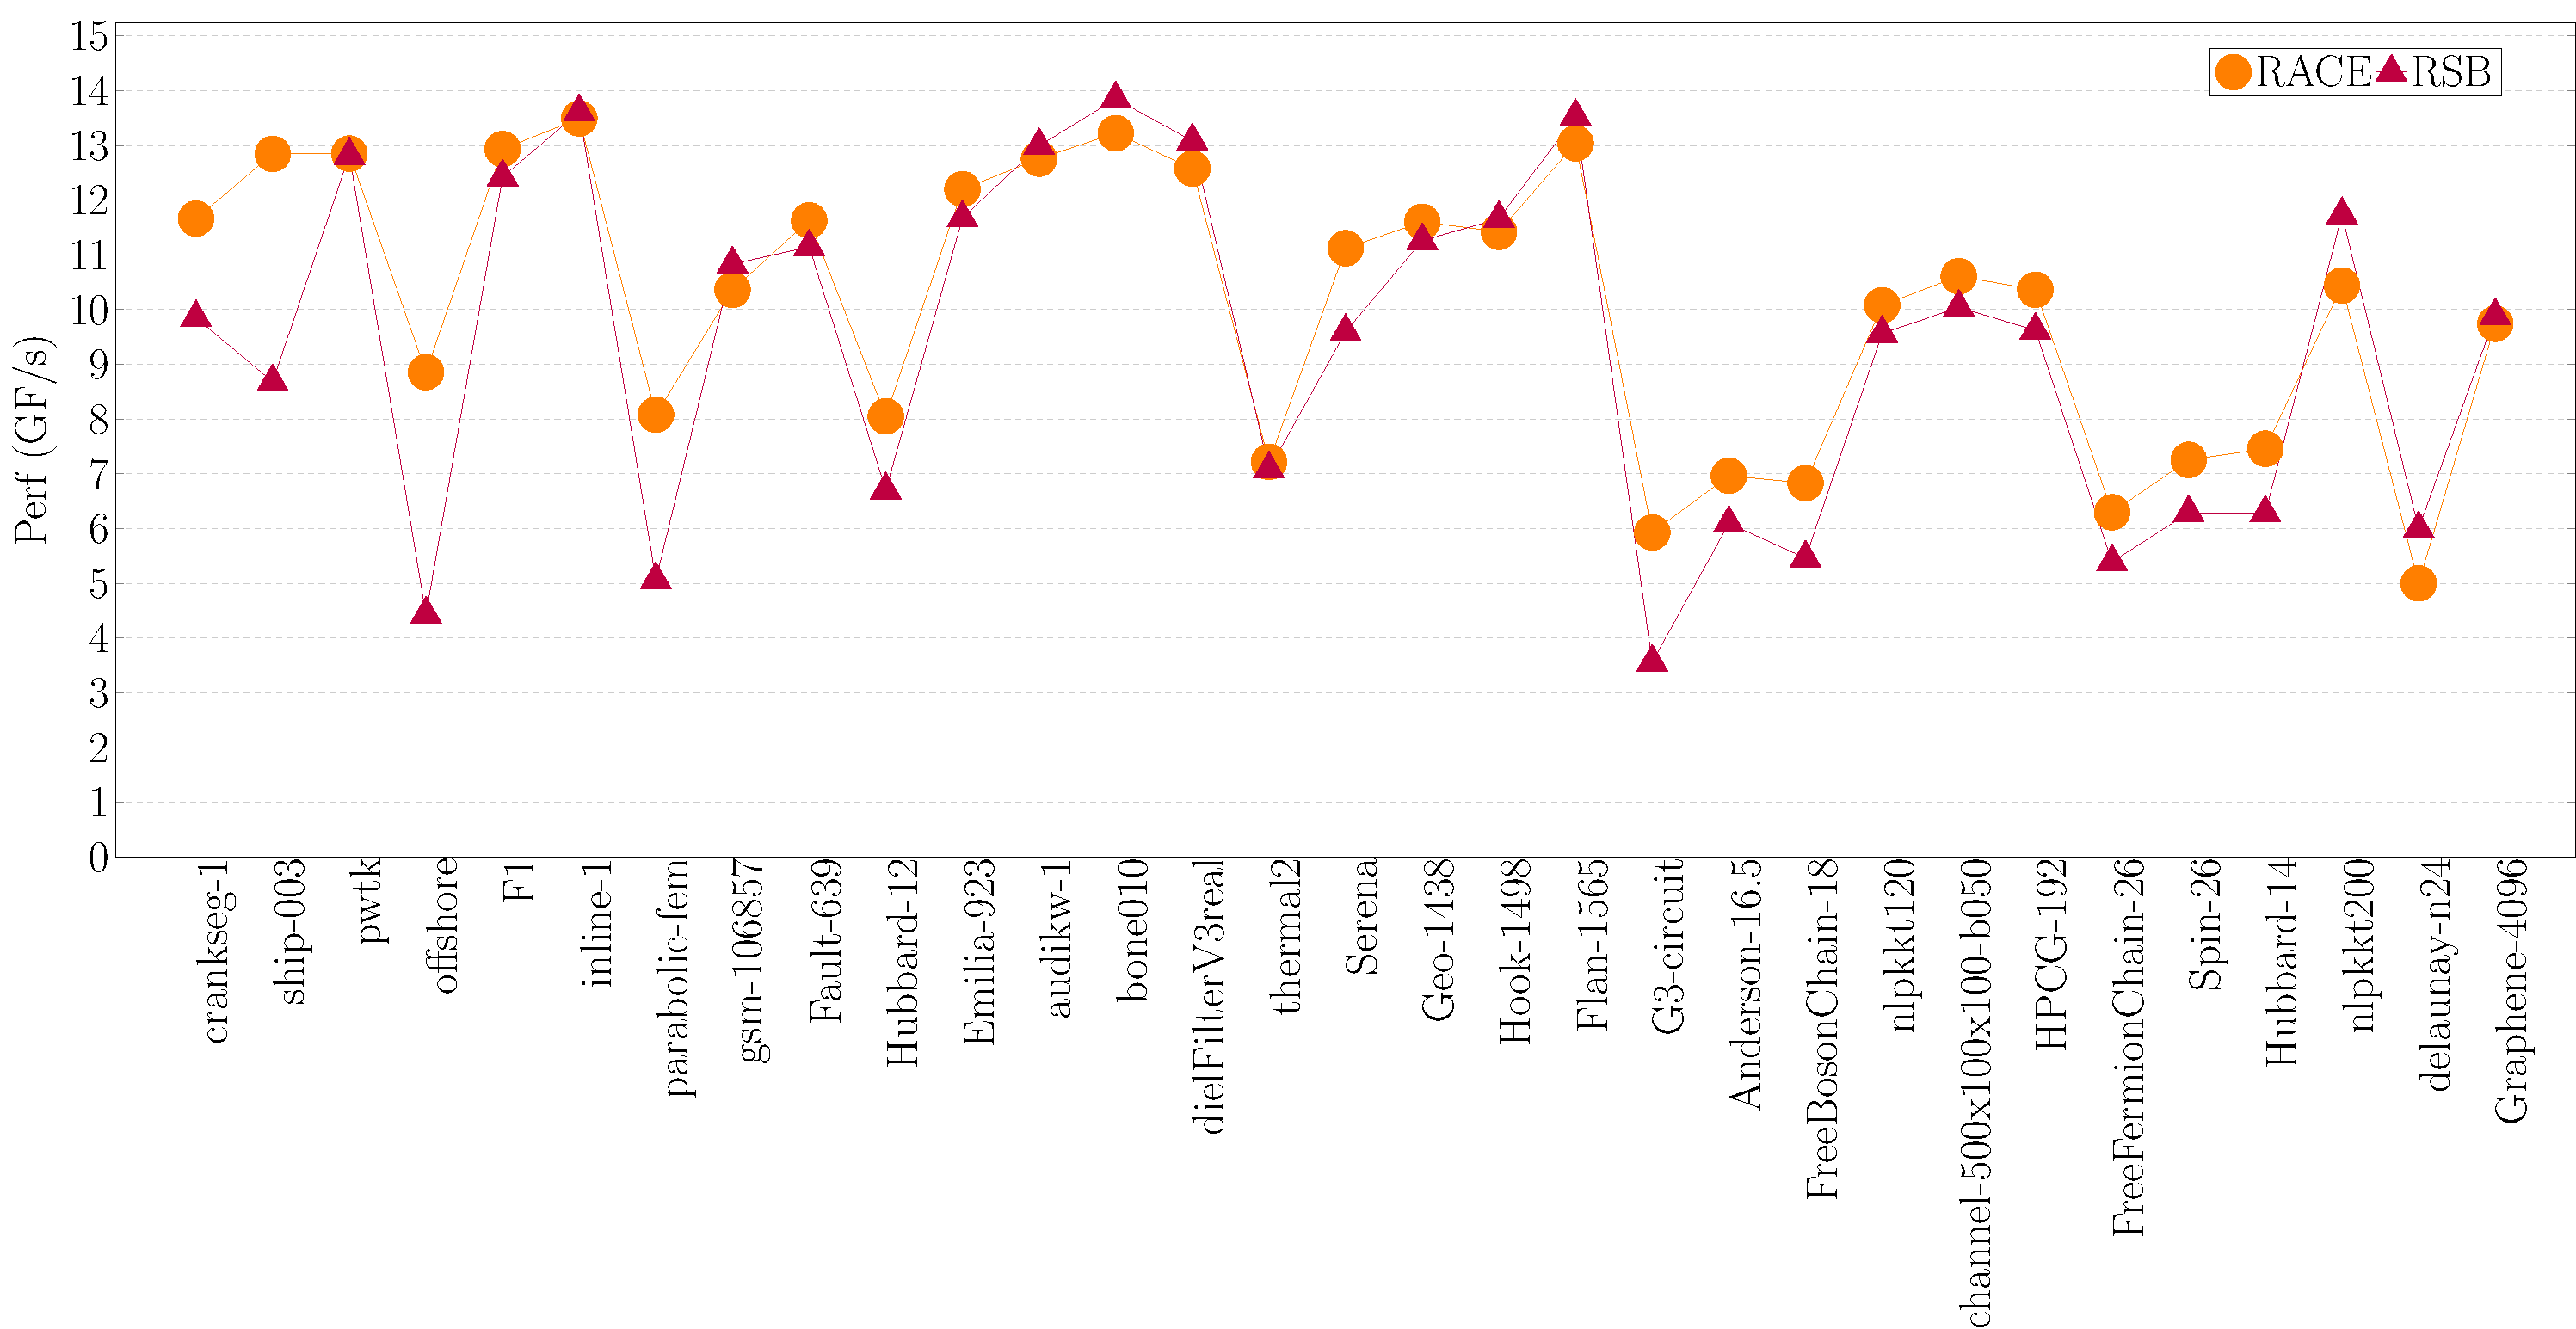
\includegraphics[width=0.45\textwidth, height=0.15\textheight]{pics/results/ivy/data_symm_spmv/plot_generator/perf_vs_mtx_w_RSB/perf}}
	\hspace{1.2em}
	\subfloat[Comparison of \acrshort{RACE} with \acrshort{RSB} on \SKX] {\label{fig:race_vs_rsb_skx}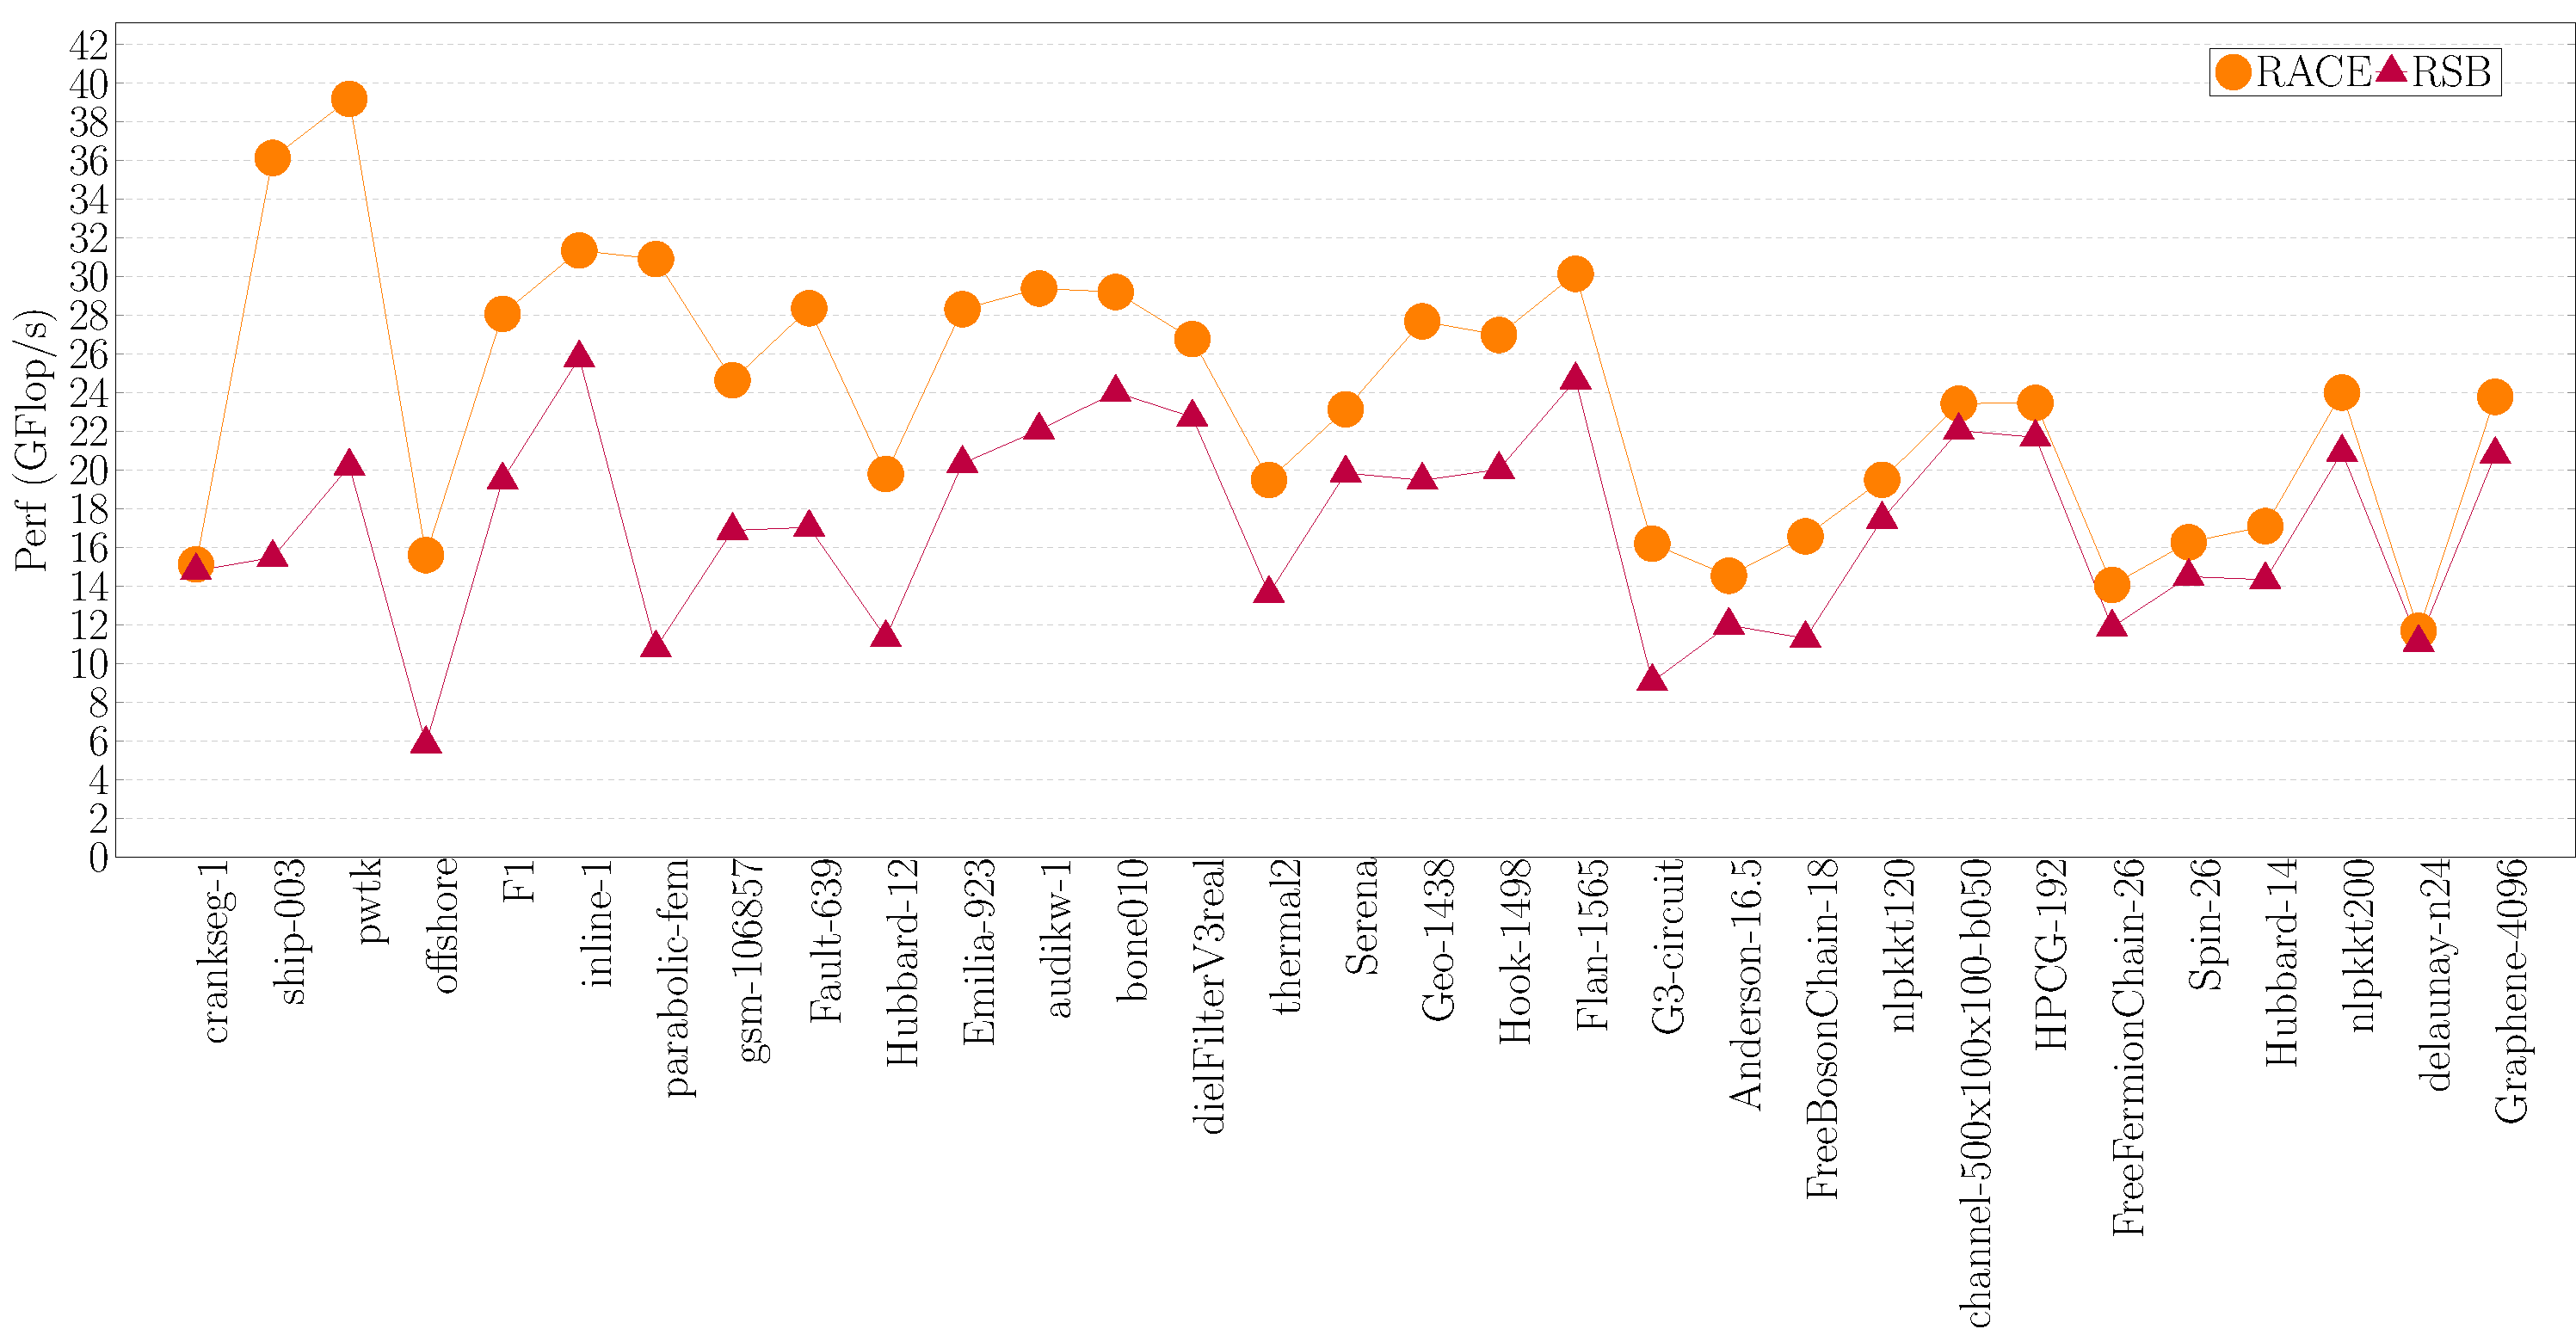
\includegraphics[width=0.45\textwidth, height=0.15\textheight]{pics/results/skx/data_symm_spmv/plot_generator/perf_vs_mtx_w_RSB/perf}}
	\caption{Comparison with \acrshort{RSB} data format}
	\label{fig:race_vs_rsb}
\end{figure}


\begin{comment}
\subsection{Main points to discuss}
\begin{itemize}
	\item Mention about specific setups like RCM for MKL and RSB, using IE for MKL
	\item Relate roofline model and the performance graphs of RACE compared to SpMV. 
	\item Point out on \IVB we reach close to ideal performance in every case, and on \SKX except for corner cases like crankseg and offshore we reach close to ideal performance. The drop in corner cases like crankseg and offshore on \SKX is due to lack of parallelism attained by RACE and associated load imbalances. This effect shows up on \SKX rather than \IVB since \SKX has 20 threads compared to 10 on \IVB.
	\item Point out that for cases like Graphene, Spin, parabolic\_fem we don't see 2 fold increase in GFlop/s for KACZ, and SymmSpMV. This is due to the fact here \acrshort{NNZR} is very small like 4, 14 and 7 which causes two problems. For KACZ kernel there is one division per row and this causes a performance drop as evident in Spin matrices, also this effect can be observed for GS kernel. For SymmSpMV kernel the \acrshort{NNZR} decreases almost by half since we operate only on upper triangular part and with short loop over \acrshort{NNZR} no effective vectorization and modulo unrolling can be done.
	\item Matrices like crankseg-1, and offshore are also really small making some part of data fit in cache, this is the reason why they achieve performance above RLM.
	\item Discuss why we chose the methods for comparison. MC and ABMC are common in literature for \DONE coloring, MKL methods are standard library used in many productive codes, also it uses level-scheduling (not explicitly stated but we believe) for kernels like GS and enables us to compare with methods that do not disturb convergence. RSB enables to compare with methods using different data format and it has been shown this method has an upper hand in this category. 
	\item Comparison with SymmSpMV shows the behavior of different methods for \DTWO coloring. Here we see in almost all of the case RACE and RSB has an upper hand on \IVB, although in some cases like offshore RACE clearly has an advantage. ABMC methods follow these methods. MKL and MC does not deliver good performance. For \SKX architecture \acrshort{RSB} falls behind \acrshort{ABMC}, we thing this is because of the requirement of \acrshort{RSB} to lock rows and cols of the submatrix on which a thread is working, becoming a bottleneck at high thread counts.
%	\item Explain SKX has slower stores, observable from load:copy benchmark ratio leading to SymmSpMV and KACZ not achieving two times SpMV, but on BDW this ratio is not much. This will get interesting with \EPY.
	\item Maybe tell RSB and 16-bit integer.
	\item Discuss with methods like ABMC and MC the performance especially drops for large matrices like Graphene, Spin, nlpkkt due to worsening of data locality ($\alpha$). Show sparsity pattern and \LIKWID meaurements. 
	\item Tell GS and KACZ performance includes also takes iterations into consideration (as shown in paper). Tell we do only a \DONE coloring for GS and \DTWO for KACZ. We use only matrices where GS can be applied and similarly for KACZ. Also we just compare against readily available solutions. Therefore RSB is left out for GS and RSB and MKL left out for KACZ.
	
\begin{figure}[thbp]
	\centering
	\subfloat[\SYMMGS iterations required by different methods compared to exact MKL kernel] {\label{fig:iter_gs}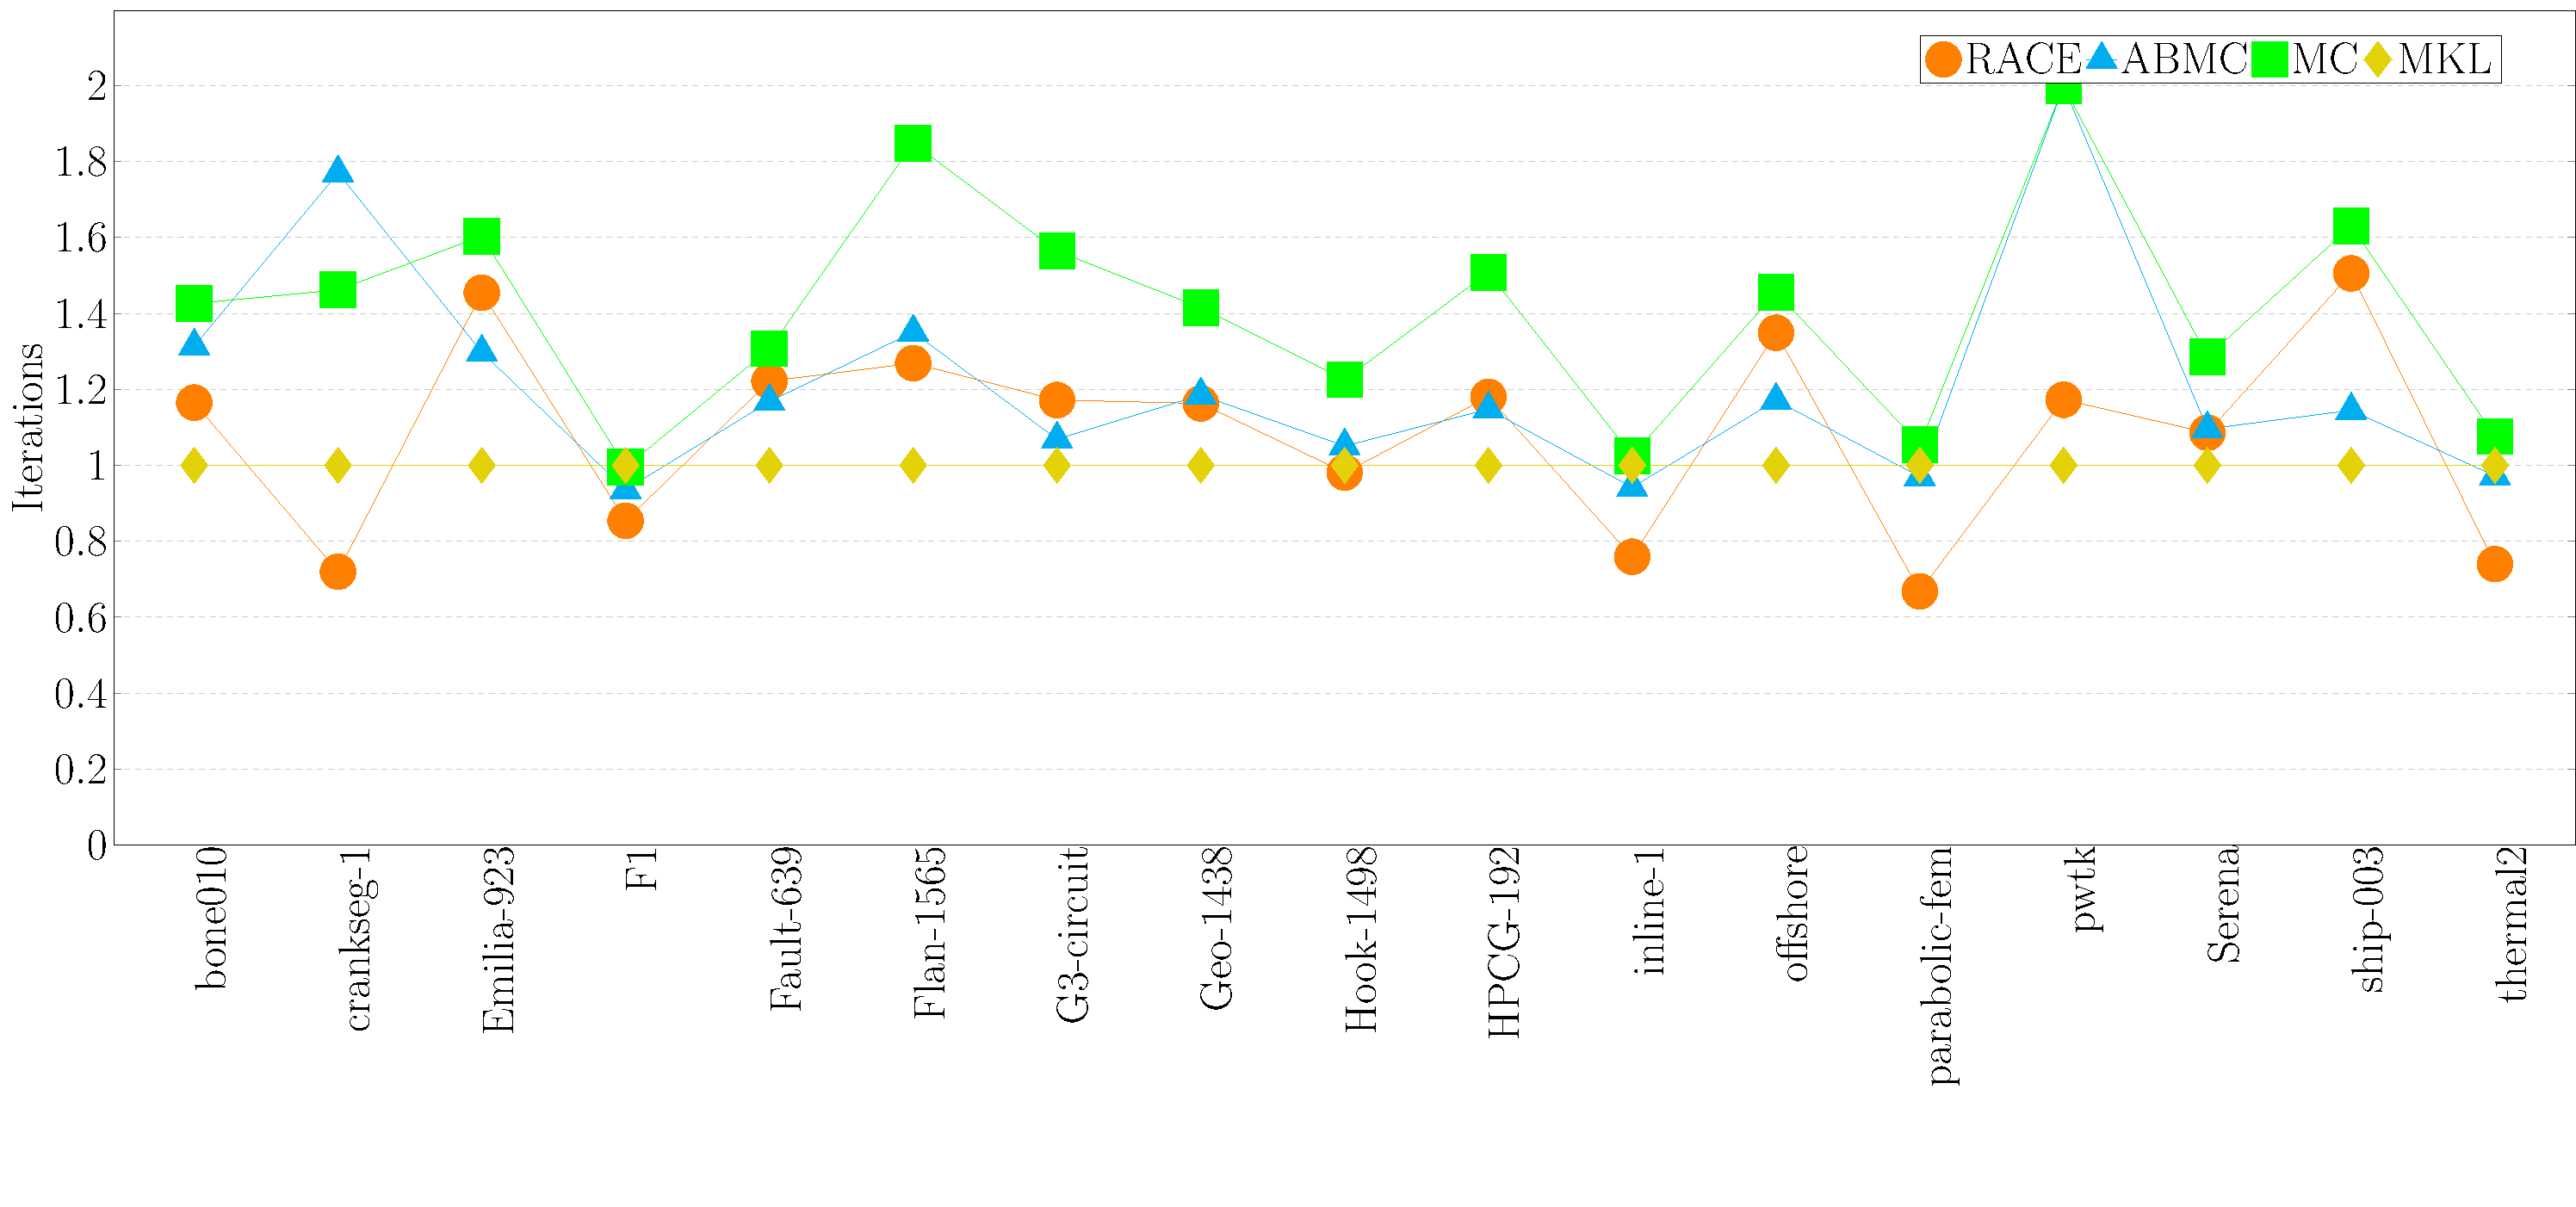
\includegraphics[width=0.49\textwidth, height=0.11\textheight]{pics/results/skx/iter/gs/plot}}
	\subfloat[\acrshort{SymmKACZ} iterations required by different methods compared to exact Serial kernel] {\label{fig:iter_kacz}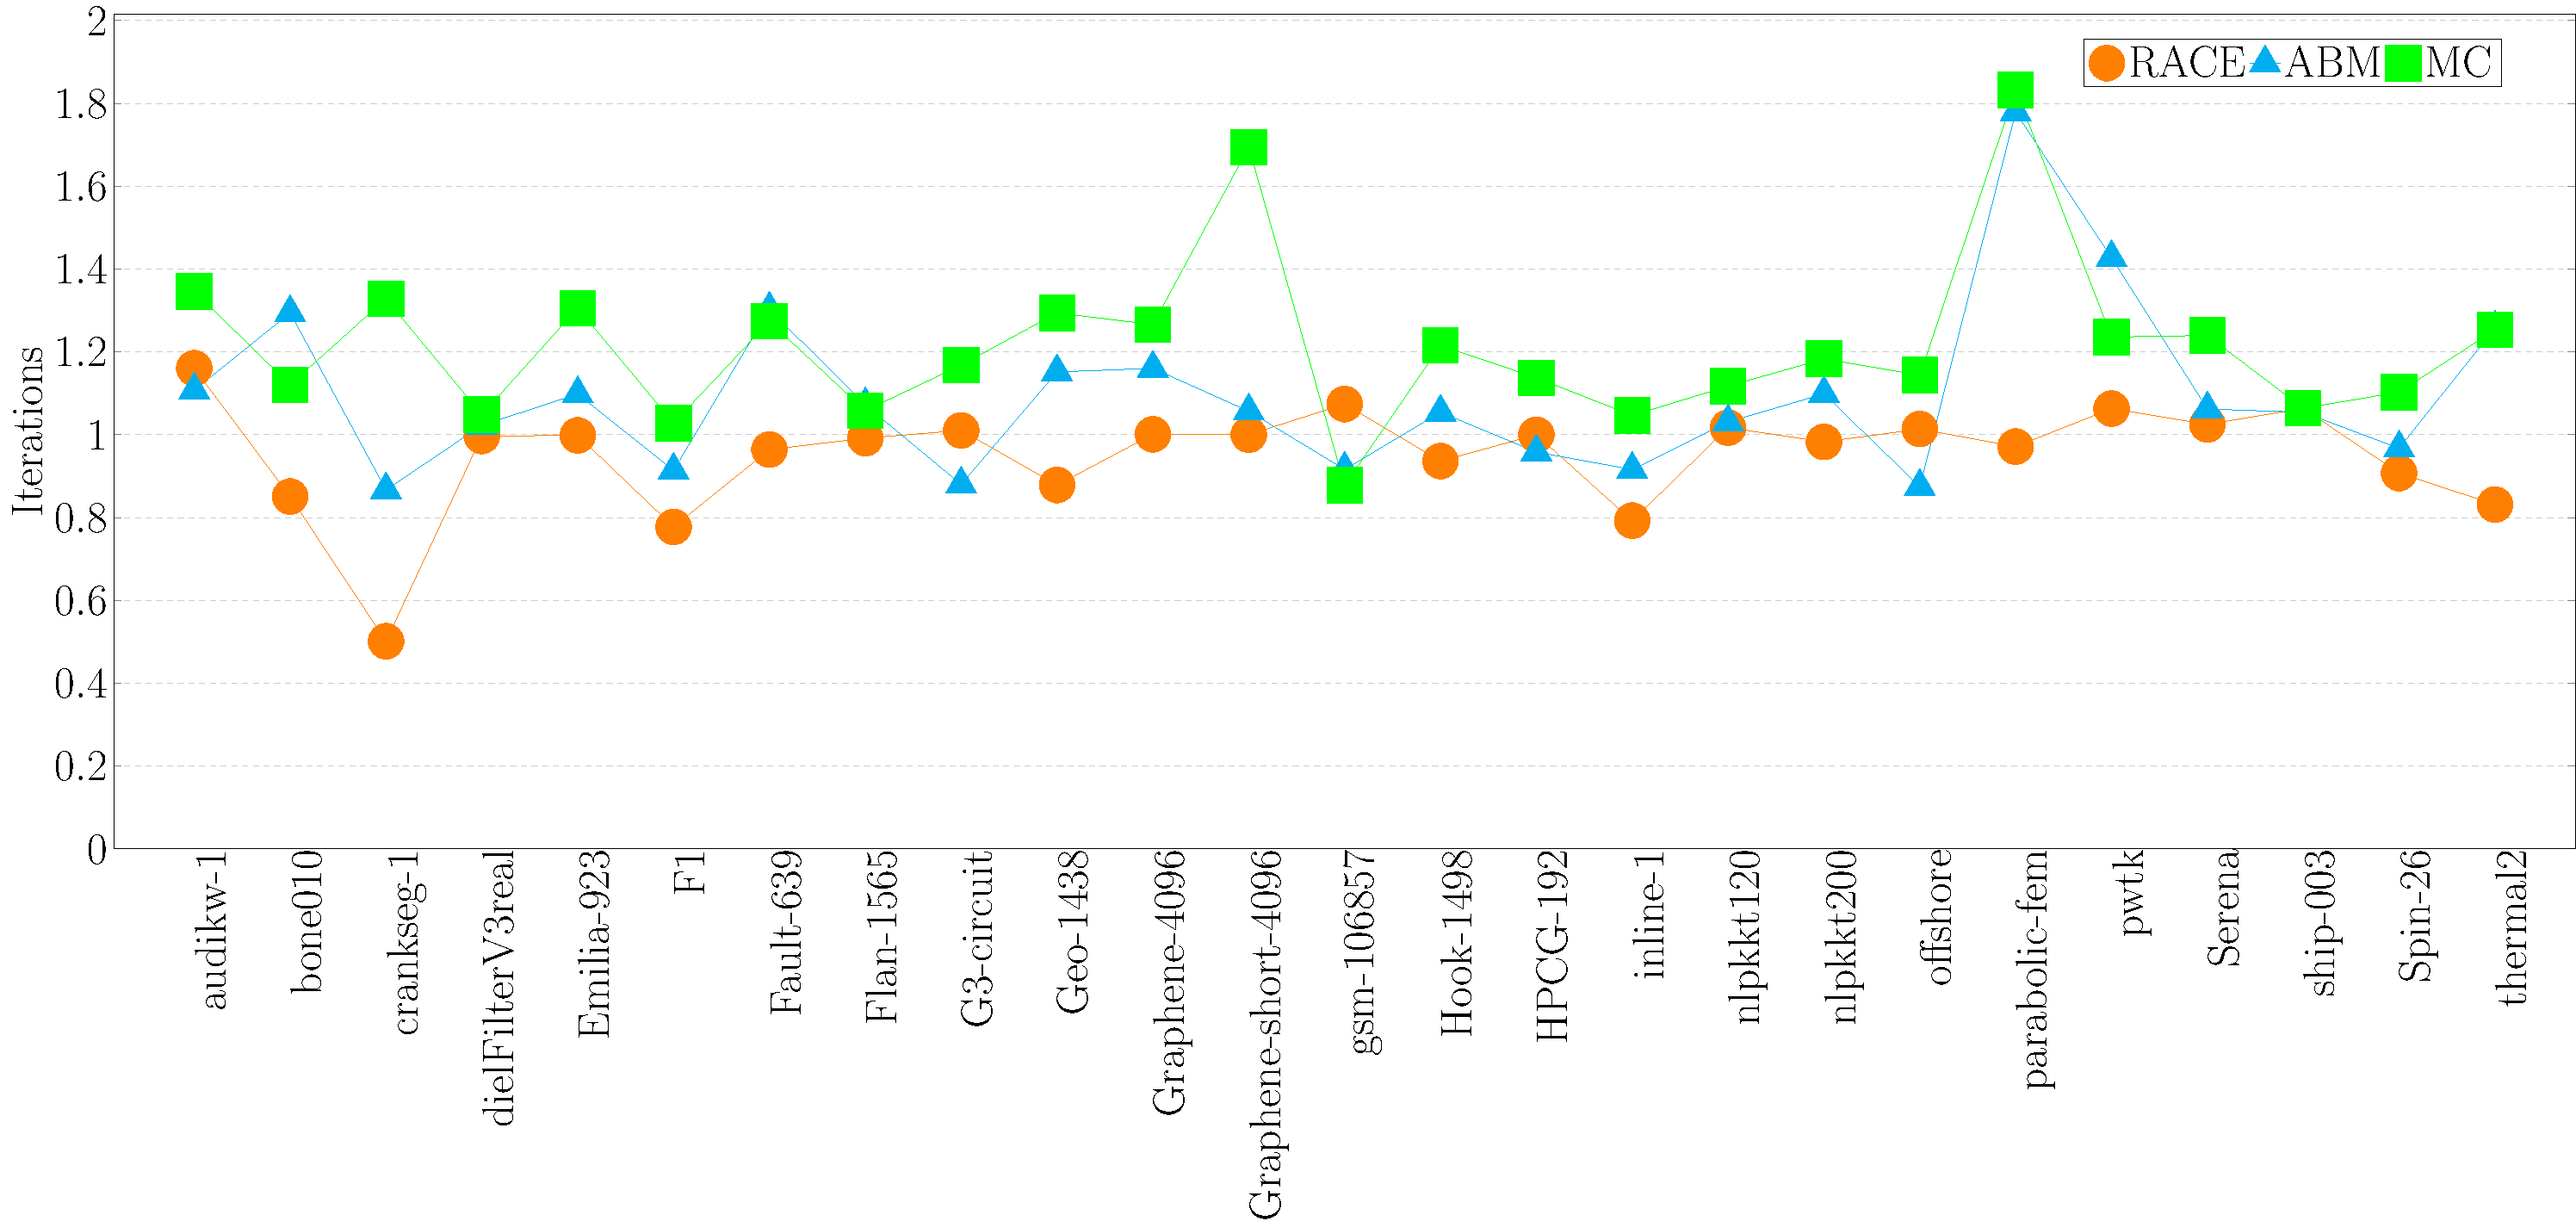
\includegraphics[width=0.49\textwidth, height=0.11\textheight]{pics/results/skx/iter/kacz/plot}}
	\caption{Convergence behavior of \SYMMGS and \acrshort{SymmKACZ} at 20 threads}
	\label{fig:conv_behavior}
\end{figure}
	
	\item For GS RACE has an upper hand on \IVB and on \SKX RACE and ABMC have almost similar performance on \SKX, although for some cases RACE has huge advantage. Reason for this advantage is due to slight decrease in iterations for RACE (see \cref{fig:iter_gs}) and slight improvement in performance compared to ABMC for \DONE case. For offshore case RACE performs worser that ABMC, this is because here with RACE one requires more iterations. Also note that all the large matrices which we had are unsuitable for GS sweep as they do not converge, but for large matrices the performance drops again for ABMC method due to degrading of $\alpha$ factor. (Maybe just put perf. pictures).
	\item Main advantage of RACE method comes with kernels having \DTWO dependencies like SymmSpMV and KACZ since here methods like ABMC require more colors and their locality degrades further since here within a color rows have to be structurally orthogonal (rows shouldn't have common column entries). Performance on KACZ shows this advantage. Here we again see for moderately large matrices the advantage is higher. Iteration behavior between methods remains similar to GS (see \cref{fig:iter_kacz}).
\end{itemize}
 
\end{comment}
